% % BEGIN OF TIKZ ONLY
% \usepackage{tikz,pgfplots}
% \usepackage{pgfplotstable}
% \pgfplotsset{compat=newest}
% \usetikzlibrary{external}
% %\tikzset{external/optimize=false}
% \tikzset{external/mode=list and make}
% \tikzexternalize[prefix=tikz/]
% \tikzsetfigurename{figure}
% \pgfplotsset{compat=newest}
\pgfplotsset{tick style={black!30},grid style={black!10}}
\pgfplotsset{every axis legend/.append style={font=\footnotesize}}
\pgfplotsset{every axis label/.append style={font=\footnotesize}}
\pgfplotsset{every tick label/.append style={font=\footnotesize}}
\pgfplotsset{every axis title/.append style={font=\footnotesize}}
\pgfplotsset{every axis post/.style={unbounded coords=jump}}
\pgfplotsset{every axis title/.append style={at={(0.5,0.95)}}}

\definecolor{LPMTrunc}{named}{TangoSkyBlue2}
\definecolor{LPMTruncInit}{named}{TangoSkyBlue2}
\definecolor{RFIR}{named}{TangoScarletRed3}
\definecolor{RFIRInit}{named}{TangoScarletRed1}
\definecolor{existing}{named}{TangoChameleon3}
\definecolor{G0Hat}{named}{TangoOrange2}
\definecolor{GVXI}{named}{G0Hat}
\definecolor{reference}{named}{black}

\definecolor{heuristic}{named}{TangoPlum2}
\definecolor{observed}{named}{TangoOrange3}

\definecolor{best}{named}{TangoAluminium6}

\definecolor{G0HatFill}{named}{TangoOrange1}
\definecolor{GVXIFill}{named}{G0HatFill}
\definecolor{LPMTruncFill}{named}{TangoSkyBlue1}
\definecolor{RFIRFill}{named}{TangoScarletRed1}
\definecolor{existingFill}{named}{TangoChameleon1}
\definecolor{bestFill}{named}{TangoAluminium3}

\definecolor{FRFMean}{named}{TangoPlum3}
\definecolor{FRFSingle}{named}{TangoPlum1}
\definecolor{FRFNoise}{named}{TangoChocolate1}

\pgfplotsset{FRFMean/.style={color=FRFMean,mark=*,mark options={solid},only marks,medsmallmarkers}}
\pgfplotsset{FRFSingle/.style={color=FRFSingle,mark=square*,mark options={solid},only marks,smallmarkers}}
\pgfplotsset{FRFNoise/.style={color=FRFNoise,mark=x,mark options={solid},only marks,smallmarkers}}

\pgfset{number format/1000 sep={\,}}

\pgfplotsset{bandwidth/.style={area style,fill=TangoButter1,draw=TangoButter2,fill opacity=0.5}}
\pgfplotsset{goodestimate/.style={color=TangoChameleon2,line join=round}}
\pgfplotsset{badestimate/.style={color=TangoScarletRed2,solid,line join=round}}
\pgfplotsset{exact/.style={color=black,dashed,line width=0.75pt,line join=round}}

\pgfplotsset{LPMTruncmark/.append style={mark=*,mark options={solid}}}
\pgfplotsset{RFIRmark/.append style={mark=square*,mark options={solid}}}
\pgfplotsset{existingmark/.append style={mark=triangle*,mark options={solid}}}
\pgfplotsset{existingInitmark/.append style={mark=triangle,mark options={solid}}}
\pgfplotsset{LPMTruncInitmark/.append style={mark=o,mark options={solid}}}
\pgfplotsset{RFIRInitmark/.append style={mark=square,mark options={solid}}}
\pgfplotsset{bestmark/.append style={mark=diamond*,mark options={solid}}}
\pgfplotsset{G0Hatmark/.append style={mark=asterisk,mark options={solid}}}

\pgfplotsset{GVXI/.style={color=GVXI,line width=1pt}}
\pgfplotsset{G0Hat/.style={color=G0Hat,line width=1.5pt}}
\pgfplotsset{existing/.style={color=existing}}
\pgfplotsset{LPMTruncInit/.style={color=LPMTruncInit,densely dashed}}
\pgfplotsset{LPMTrunc/.style={color=LPMTrunc}}
\pgfplotsset{RFIRInit/.style={color=RFIRInit,densely dashed}}
\pgfplotsset{RFIR/.style={color=RFIR}}
\pgfplotsset{best/.style={color=best}}

\pgfplotsset{smallmarkers/.append style={mark size=0.75pt}}
\pgfplotsset{medsmallmarkers/.append style={mark size=0.5pt}}
\pgfplotsset{tinymarkers/.append style={mark size=0.25pt}}
\pgfplotsset{extremelytinymarkers/.append style={mark size=0.05pt}}


\tikzset{annotation/.style={align=left,draw=black!0.2,font=\scriptsize,fill=white,fill opacity=0.8}}
% http://tex.stackexchange.com/questions/83487/pgfplotstable-converting-zeros-to-in-a-knitr-inline-table
\pgfplotstableset{%
	zerofill=true,
	after row=[3pt],
                  every head row/.style={before row=\toprule, after row={\\\midrule}},
                  every last row/.style={after row=\bottomrule}
	assign column name/.code={%
        \pgfkeyssetvalue{/pgfplots/table/column name}{\multicolumn{1}{c}{\multirow{2}{*}{#1}} }%
    },
	columns/method/.style={string type,column name={\shortstack{\textsc{Method}\\\phantom{0}}}},
	columns/P000/.style={column type=r,column name={\shortstack[r]{\textsc{Min.}\\{$0\%$}}}},
	columns/P025/.style={column type=r,column name={\shortstack[r]{\vphantom{?}\\\textsc{$25\%$}}}},
	columns/P050/.style={column type=r,column name={\shortstack[r]{\textsc{Median}\\{$50\%$}}}},
	columns/P075/.style={column type=r,column name={\shortstack[r]{\vphantom{?}\\\textsc{$75\%$ }}}},
	columns/P100/.style={column type=r,column name={\shortstack[r]{\textsc{Max.}\\{$100\%$}}}},
	columns/contribution/.style={column name={\shortstack[r]{\textsc{Contribution}\\ \vphantom{0}}},
                    	postproc cell content/.append code={\pgfkeysalso{@cell content/.add={}{\%}}},
	}
}

% % END OF TIKZ ONLY
% \newcommand{\legref}[2][1]{(\ref{#2})}

%  \newlength\figureheight
%  \newlength\figurewidth
%  \setlength\figureheight{7cm}
%  \setlength\figurewidth{10cm}

%  \newlength\onecolumnwidth
%\title{Improved Initial Estimates Via FRF Smoothing Techniques for Parametric Identification of LTI Systems}

% \begin{abstract}
% Good initial values are crucial to obtain solutions of non-convex optimization problems. When estimating the transfer function of physical systems from measured noisy data, obtaining good initial parameter estimates is therefore a primordial step.
% In this paper, it is shown that smoothing the measured frequency response function (FRF) of a linear time-invariant system enhances the construction of initial estimates significantly, resulting in the optimization schemes to converge to a better optimum. 
% This is achieved with minimal user interaction.

% Two smoothing techniques, the time-truncated local polynomial method (LPM) and the regularized finite impulse response (RFIR), are compared with the existing generalized total least squares (GTLS) and the bootstrapped total least squares (BTLS) initial estimates. 
% The improvement attributable to smoothing is demonstrated by a simulation and by measurements of an electrical filter. 
% The results ultimately show that the parametric models obtained using the proposed starting values are much more likely to give a good description of the measured system and hence lead to more useful models.
% \end{abstract}

\setlength\onecolumnwidth{\columnwidth}

\TODO{import references into main bibliography}
%\comment{JL: 
%Focus of the article (this is what the article must reflect):

%\begin{itemize}
%\item demonstrate that a smoothed FRF, obtained as described in \citep{Lumori2014}, used as an initial estimate increases the success rate of a parametric LTI TF identification
%\item
%\comment{JL:  emphasize the importance of extending the SNR range for which the success rate is acceptable, yielding a reliable parametric estimator to be used with as little user interaction as possible.
%\end{itemize}
%}

\section{Introduction}\label{se:introd}

The task of interpreting measurement data from dynamic systems often involves the estimation of a transfer function (TF). 
Typical measurement techniques and identification strategies of transfer functions (TFs) or \glspl{FRF} are discussed in \citep{Schoukens1998,Schoukens2006LPM,Guillaume1996,Broersen1995,Pintelon2010LPM1,Antoni2007FRF}.
Application of these methods to real devices and systems is well-known in published literature, including \citep{Lim2010,Robinson1990,Behjat2010}.

Parametric identification of \gls{LTI} systems from input/output data has been well developed as evidenced by published literature~\citep{Pintelon2012,Ljung1999,Schoukens1999,Pintelon1998}. 
 Maximizing the likelihood function of the parameters probably yields the most popular, consistent and efficient estimator. 
 However, in a noisy environment, the \gls{MLE} engenders a nonlinear optimization which, at the very least, requires good initial estimates to avoid local optima.
 Such local optima have a detrimental effect on the quality of the estimated model.

 In the perspective of developing identification tools that require as little user interaction as possible, it is important to increase the probability of the optimization algorithm to produce good estimates, or preferably even the global optimum.
 However, when noisy input-output measurements are to be processed, the presence of noise obstructs a clear view of the actual system behavior, especially for poor signal-to-noise ratios (SNRs).
 In non-parametric identification, the presence of noise is typically mitigated by averaging multiple measurements or using smoothing techniques.

The main aim and contribution of this article is to demonstrate that smoothing a measured \gls{FRF} helps to avoid local optima during the parametric estimation of the \gls{MLE} of a transfer function, using deterministic optimization algorithms.
Hence, such techniques make it possible to increase the ``success rate'' (i.e. the probability that a good model, or even the global optimum, is obtained) of such a system identification step considerably.
%Such techniques, hence allow to increase the ``success rate'' (i.e. the probability that a good model, or even the global optimum, is obtained) of such a system identification step considerably.

In particular, two different smoothing techniques --- the time-truncated \gls{LPM}~\citep{Lumori2014TIM} and the \gls{RFIR}~\citep{Pillonetto2010,Chen2012} --- are tested for different \glspl{SNR} and different measurement record lengths of the input/output data of a few \gls{SISO} \gls{LTI} systems.
These are compared with the existing initialization schemes, namely: (i) the \gls{GTLS}, and (ii) the \gls{BTLS}.
%The existing initialization schemes compared with are the generalized total least squares (GTLS) and bootstrapped total least squares (BTLS).

The rest of the paper is structured as follows. Section~\ref{se:ProbForm} covers the problem formulation. Section~\ref{se:MethodEg} discusses the methodology for obtaining the initial estimates, and their influence on the success rate of the \gls{MLE}. 
This is followed by Sections~\ref{se:Demo} and \ref{se:ExpMeas}, which are demonstrations of the improved initial estimates by simulation and experimental data, respectively.
In Section~\ref{se:Generality} the generality of the results is discussed briefly.
Ultimately, concluding remarks are presented in Section~\ref{se:Conclusion}.

% !TEX root =  InitialValuesPaper.tex

\section{Problem formulation}\label{se:ProbForm}
%\begin{itemize}
%\item
%Block schematic of the output error framework

%\JL{In this section, the assumptions on the system and the noise are given, and the associated Maximum Likelihood estimator, formulated in the frequency domain. The latter turns out to be a non-convex function in the parameters, requiring initial estimates. The obtention of those is discussed in the subsequent section.}

In this section, the assumptions on the system and the noise are presented, together with the associated MLE (formulated in the frequency domain), which turns out to be a non-convex function in the parameters, requiring initial estimates. The procedure for obtaining the initial estimates is discussed in the subsequent sections.

\subsection{System Setup Framework and Model}
\figref{fig:oesetup} depicts a schematic of the output error framework for  a generalized (single- or multiple-order) resonating, dynamic LTI discrete-time SISO system, subjected to a known white random noise input. The following mathematical derivations pertain to discrete time systems, but they can be extended to continuous time systems as well. The full mathematical model of the system is
\begin{equation}\label{lpmtd1}
y(t)=G_0(q^{-1})u_0(t)+H_0(q^{-1})e(t)
\end{equation}
%\comment{We don't have any results with colored noise yet!}
where $G_0(q^{-1})$ represents the dynamics of the system to be estimated, $u_0(t)$ is the input signal, $v(t)= H_0(q^{-1})e(t)$ is the noise source at the output, $H_0(q^{-1})$ is the noise dynamics, 
%\comment{JL: note that $H_0 = 1$ in this paper, so only white noise is considered, i.e. $e(t) = v(t)$.}, 
$e(t)$ is white Gaussian noise, and $q^{-m}$ is the backwards shift operator ($q^{-m}x(t)$ = $x(t-mT_{\mathrm{s}})$  with $m$ a positive integer and $T_{\mathrm{s}}$ the sampling time).
For white noise, $H_0 = 1$ and $e(t) = v(t)$.
Note that for simplicity, we only treat the discrete-time case (i.e. $t = n \cdot T_{\mathrm{s}}$ for integer values of $n$) theoretically in this paper.
However, the generalization to continuous time is straightforward~\citep[Chapter 6]{Pintelon2012} and has been demonstrated in Section~\ref{se:ExpMeas}.

\begin{figure}[tbh] %top bottom here
\centering
\tikzstyle{block}     = [draw,rectangle,minimum height=2em,minimum width=1.5em,inner sep=2mm]
\tikzstyle{sum}       = [draw,circle,inner sep=0mm,minimum size=2mm]
\tikzstyle{input} = []
\tikzstyle{output} = []
\tikzstyle{pinstyle} = [pin edge={<-,black},color=black]

\begin{tikzpicture}[auto, node distance=2cm,>=latex]

    \node [near start] (input) {$\true{u}(t)$};
    \node [block, right of=input] (system) {$\true{G}(q^{-1})$};
    \node [sum, right of=system,
           node distance=2.2cm] (sum) {\footnotesize$+$};
    \node [right of=sum, node distance=1.3cm] (output) {$y(t)$};

    \node [above of=sum, node distance=1.3cm] (noise) {$v(t)$};

    \draw [->] (input)  --   (system);
    \draw [->] (system) -- node[name=y0] {$\true{y}(t)$} (sum);
    \draw [->] (sum)    --    (output);

    \draw [->] (noise) -- (sum);

\end{tikzpicture}

\caption[Output-error set-up.]{SISO LTI discrete-time system in an output error setup.}
\label{fig:oesetup}
\end{figure}

Numerous parametric identification techniques are devoted to the development of parametric plants $G(q^{-1},\theta)$ and parametric noise models  $H(q^{-1},\theta)$, where  $\theta$ is the model parameters vector  \citep{Ljung1999,Soderstrom1989}.

The output signal is disturbed by white random noise, resulting in noisy error-prone data. It is also possible to apply the estimation procedure in this paper to a system that is disturbed by colored noise, as will be demonstrated in Section~\ref{se:ExpMeas}. 

\subsection{Parametric System Model}

With reference to equation (\ref{lpmtd1}), the relation between the noiseless input and the output signals ($v(t)= 0$) is assumed to be of the form
\begin{equation}
    A(q^{-1}) y_0(t) = B(q^{-1}) u_0(t)
\label{ABpolys}
\end{equation}
where $A$ and $B$ are polynomials in $q^{-1}$. Thus, it follows from equation (\ref{lpmtd1}) that
\begin{equation}
    G_0(q^{-1})= \frac{B(q^{-1})}{A(q^{-1})}
    \text{.}
\end{equation}

From~\citep[Section 6.3.2.]{Pintelon2012}, in the frequency domain, and for the DFTs (Discrete Fourier Transforms) of the windowed signals, equation \eqref{ABpolys} is of the form
\begin{align}
A(e^{-j\omega_k})Y_0(k) = B(e^{-j\omega_k})U_0(k) + I(e^{-j\omega_k})
\label{DFTspectra}
\end{align}
with $q^{-1}$ sampled in  $q_k^{-1} = e^{-j\omega_k}$, where $\omega_k = \frac{2\pi k}{N}$ are the DFT frequencies, and $I$ is a polynomial of order $\max(N_a,N_b) - 1$, which depends on the initial and end conditions. 
In this paper, it is assumed that the orders of the polynomials $A$, $B$ and $I$ are known.

\subsection{Parametric Identification Algorithm}\label{se:paramIdentAlgo}

The maximum likelihood estimate of the parameter vector $\theta$  containing the coefficients of the $A$, $B$ and $I$  polynomials is obtained by solving the optimization problem
\begin{equation}
  \hat{\theta} = \arg\min_\theta V(\theta) \text{.}
\end{equation}
Since the noise $v(t)$ is assumed to be Gaussian, $V(\theta)$ accords to the weighted least squares cost function~\citep[Section 9.11]{Pintelon2012}:
\begin{equation}\label{eq:MLEcf}
V(\theta) = \sum_{k=1}^{N/2-1}\frac{|\varepsilon(k,\theta)|^2}{\sigma_\varepsilon^2(k,\theta)}
\end{equation}
for $N$ measurements and when $\varepsilon$ denotes the error in equation (\ref{DFTspectra}),  \emph{viz}.:
\begin{align}
\varepsilon(k,\theta) = A(k,\theta)Y(k) - B(k,\theta)U(k) - I(k,\theta)\text{.}
\end{align}
The variance of the error is of the form:
\begin{equation}\label{eq:sigmaEps}
\begin{split}
\sigma_\varepsilon^2(k,\theta) 
  &=  |A(k,\theta)|^2\sigma_Y^2(k) 
   +  |B(k,\theta)|^2\sigma_U^2(k) \\
  &- 2\;\mathrm{real} \left( A(k,\theta) \overline{B(k,\theta)} \sigma_{YU}(k) \right)
\end{split}
\end{equation}
where $\sigma_Y^2$ is independent of $k$ for white noise, %assumed to be a known error variance \comment{JL: why should the error variance be known? where do you use that? how do you compute it?} of the measured output spectrum $Y$ \comment{JL: relate the output error variance with the variance of $v(t)$. Isn't it the same thing?},
%\comment{this is true for white noise, and for the scaling of the DFT by $\sqrt{N}$. I think it is more clear to use the frequency domain variance instead: $\sigma_Y^2$}
and the input error variance is assumed to be zero, i.e. $\sigma^2_U=0$, and similarly, the covariance $\sigma_{YU} = 0$.
Here, $\overline{B}$ denotes the complex conjugate of $B$.
%\comment{use $\sigma^2_U$ instead}

Consequently, $V(\theta)$ is a non-quadratic function of $\theta$ which, in general, results in a non-convex optimization problem. 
The Levenberg-Marquardt~\citep{Marquardt1963} algorithm (see Algorithm~\ref{LMalgo}) is used to solve this optimization problem deterministically.
Such an approach requires good initial estimates of $\theta$ to avoid inherent local optima, which is the focus of this paper.

\begin{algorithm}
\caption{Levenberg-Marquardt~\citep{Marquardt1963}, \citep[Sec. 9.L.4]{Pintelon2012}}\label{LMalgo}
\begin{algorithmic}[1]
  \Statex Cost function \eqref{eq:MLEcf} is rewritten as $V(\theta) = \epsilon^{\TT} \epsilon$. 
  \Statex The iterations start at $\atIter[0]{\theta} = \theta^{\mathrm{init}}$ and $\lambda = \max(\sigma)/100$.
%\Function{LevenbergMarquardt}{$V(\theta), \atIter[0]{\theta}$}
   \For{$i$ \textbf{in} $1 \to \infty$}
      \State $U \, \Sigma \, W^{\TT} \gets \mathtt{svd}\left( \frac{\partial \epsilon}{\partial \theta}\right)$ with $\mathrm{diag}(\Sigma) = [\sigma_1, \ldots, \sigma_n]$
      % \State \textbf{if} $i=1$ \textbf{ then} $\lambda \gets \max(\sigma) / 100$
      \State $\sigma_k \gets \sigma_k / (\sigma_k^2 + \lambda^2) \quad \forall k \in \{1, \ldots, n\}$
      \State $\delta\theta \gets - W  \Sigma^{\TT}  U^{\TT} \epsilon$
      \State $\atIter[i]{\theta} \gets (\atIter[i-1]{\theta} + \delta\theta) / \norm{\atIter[i-1]{\theta} + \delta\theta} $
      \If{$V(\atIter[i]{\theta}) > V(\atIter[i-1]{\theta})$}
          \State $\lambda \gets 10 \lambda$ and then retry at $i \gets i - 1$
      \Else
          \State $\lambda \gets 0.4 \lambda$
      \EndIf
      \State \textbf{if} $\norm{\delta\theta}/\norm{\atIter[i]{\theta}} < n_{\theta}  \cdot 10^{-6} $ \textbf{then} \textbf{return} $\hat{\theta} \gets \atIter[i]{\theta}$
   \EndFor
%\EndFunction
\end{algorithmic}
\end{algorithm}

\begin{remark}
Alternatively, stochastic optimization algorithms~\citep{Spall2012,Press2007} are less likely to get stuck in local optima since many randomized initial estimates are tried.
This obviously comes with a huge computational cost compared to `classical' deterministic schemes where only a single or a few initial estimates are used to start the expensive iterative optimization procedure.
Stochastic optimization is not discussed in the remainder of this paper.
\end{remark}

\section{Methodology}\label{se:MethodEg}
In this section, the considered methods for obtaining the initial estimates of $\theta$ are briefly explained. Then their influence on the success rate of the maximum likelihood estimator is described.
%}

\subsection{Initial Estimates Procedure}\label{se:initEstProcs} %{Obtaining initial estimates}

%\begin{itemize}
%\item
%Obtain a good estimate of the FRF of the system by using the LPM: short description + reference

\begin{figure}
  \centering
  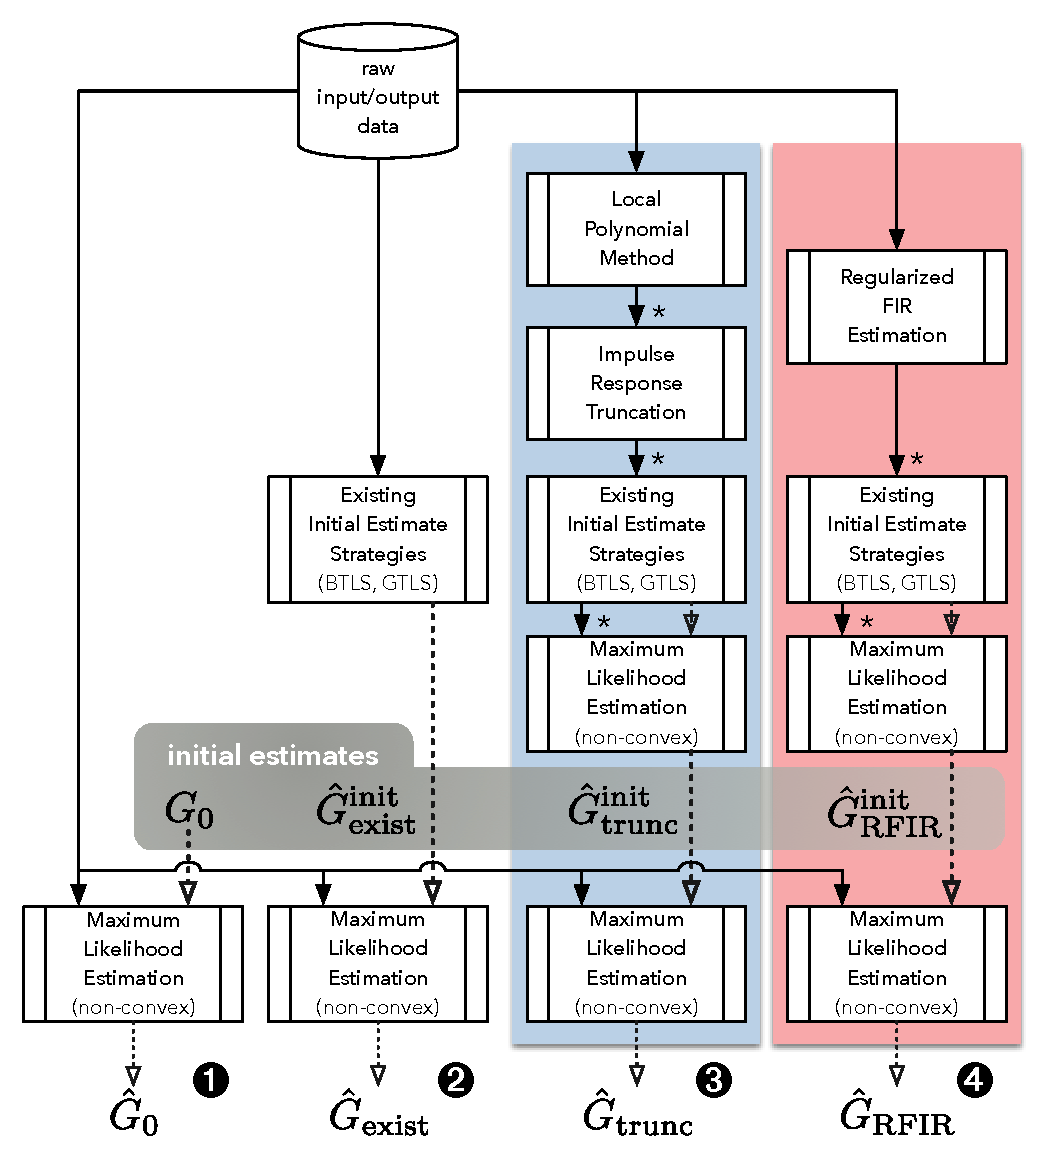
\includegraphics
  [width=0.95\onecolumnwidth]{\thisDir/fig/flowgraph}
  \caption[Flow chart of different initialization procedures.]{Flow chart depicting the different estimation procedures, from left to right: (1) an approach using the true model as initial estimate; (2) an existing approach using \gls{BTLS} and \gls{GTLS} starting values, and the novel methods outlined in this paper (3, 4).
  The flow of non-parametric data is depicted by full arrows, with the \gls{FRF} data marked by asterisks. Parametric models are indicated by dashed, unfilled arrows.} \label{fig:flowgraph}
\end{figure}

The ultimate aim is to find initial estimates that are good enough to steer clear of the local optima during the \gls{MLE} optimization process in the parametric identification of each system. 
The requisite procedures for the estimators are as follows, from left to right of the flowchart in \figref{fig:flowgraph}:


\begin{enumerate}
\item
\emph{Using the true model ($G_0$) as initial estimate}

The estimates from this procedure are for comparison purposes with those from the other procedures. They will be crucial to the computation of the global optimum of the \gls{MLE}.

\item
\emph{Quadratic approximations of the ML}

%\JL{The Generalized Total Least Squares (GTLS) and the Bootstrapped Total Least Squares (BTLS) have been discussed in \citep{pintGuil1998}. These are modifications of \eqref{eq:MLEcf}, which still take into account the noise information, while keeping the quadratic nature w.r.t.\ $\theta$. These estimators preserve consistency (which is an asymptotic behaviour, i.e.\ for $N\to\infty$). Their finite sample behaviour is prone to be improved by the FRF smoothing tools, described below.}

The \gls{GTLS} and the \gls{BTLS} have been discussed in \citep{Pintelon1998}. These are modifications of equation \eqref{eq:MLEcf}, which still take into account the noise information while retaining the quadratic nature w.r.t. $\theta$. 
These estimators preserve consistency, such that the estimates converge asymptotically to the true parameters for $N\to\infty$. 
Their finite sample behavior, however, is suitable for improvement by the \gls{FRF} smoothing tools as described below.

\item
\emph{Local polynomial method (LPM) with truncation}

A reliably good estimate of the FRF of the chosen system can be obtained via the LPM, which is summarized as follows~\citep{Lumori2014TIM}. Formulated as a nonparametric linear-least-squares-estimate, the LPM is first applied to estimate the FRF from a full data record of a SISO system, systematically expressed in an output-error framework, shown in \figref{fig:oesetup}. The smooth characteristics of both the exact \gls{FRF} $G_0$ and the transient term $T$ allow for an optimal application of the \gls{LPM}, leading to a smooth \gls{FRF} estimate with the transient suppressed.

  With reference to a detailed discussion in~\citep{Lumori2014TIM}, the \gls{LPM} utilizes the following quadratic local polynomials to approximate (in least squares sense) and, thus, smooth $G_0$ and $T$ around a central frequency $\Omega_{k}$ in a local frequency band $r\in\mathbb{W}_n$
\begin{subequations}\label{lpmImplQuadG}
\begin{align}
G_0(\Omega_{k+r})&\approx \hat G_k + g_{1,k} r + g_{2,k}r^2
\\
T(\Omega_{k+r})&\approx T(\Omega_k)+t_{1,k}r + t_{2,k}r^2\label{lpmImplQuadT}
\end{align}
\end{subequations}
where, in general,$\ r\in\mathbb{W}_n,\quad$$\mathbb{W}_n = \{-n,-n+1,\dots,n\}$ and $n$ is a tunable parameter. In this paper, $n=3$.

  The \gls{LPM} estimate of the \gls{FRF} at frequency index $k$ is the first estimated local parameter, \emph{viz}:
\begin{equation}
\hat{G}_\text{poly}(\Omega_k) = \hat{G}_k
\text{.}
\end{equation}
This procedure is repeated for all $k$ in the frequency band of interest.

%The estimation of $\hat{G}_\text{poly}(\Omega_k)$ at a single frequency $\Omega_k = 0.586$~Hz is illustrated in Fig. \ref{LPM_Schematic_EG}.

\emph{Impulse response truncation}. 
%\comment{JL: in this paper, the impulse response truncation as an initial estimator is considered together with the LPM. So I would not start a new subsection for it.}
The estimate is smoothed further by truncating its impulse response function $g_{\text{poly}}(t) = \mathrm{IDFT}\, \left( \hat{G}_\text{poly}(\Omega_k)) \right)$ as originally presented in~\citep{Lumori2014TIM}.
%\comment{JL: $\hat{G}_\text{poly}(\Omega_k))$ is undefined}.

The impulse response is truncated after the time $\tau_{\mathrm{trunc}}$ where the signal becomes indistinguishable from the noise, i.e.
\begin{equation}
  g_{\mathrm{trunc}}(t) = 
  \begin{cases}
    g_{\text{poly}}(t) & t \leq \tau_{\mathrm{trunc}} \\
    0                    & t \geq \tau_{\mathrm{trunc}}
  \end{cases}
  \text{.}
\end{equation}
To this end, an estimate of the envelope of impulse response is determined by fitting an exponential function $g_{\mathrm{exp}}(t) = B e^{\beta t}$ to the peaks of the impulse response $\abs{g_{\mathrm{poly}}(t)}$ using a linear least-squares approach.
Then, $\tau_{\mathrm{trunc}}$ is determined as the time instant where this envelope function sinks below the noise level $\sigma_g$ of the impulse response, i.e. 
\begin{equation}
  \tau_{\mathrm{trunc}} = \min \left\{  t :  g_{\mathrm{exp}}(t) < \gamma \sigma_g \right\}
  = \beta^{-1} \ln \frac{\gamma \sigma_g}{B}
  \text{,}
\end{equation}
where $\gamma=1$ was used in this paper for simplicity.
By changing $\gamma$, the user can fine-tune the bias/variance trade-off of the estimated FRF $G_{\mathrm{trunc}}(\Omega_k) = \mathrm{DFT} \left( g_{\mathrm{trunc}}(t)\right)$ further.
This can lead to a significant improvement over the classical LPM~\citep{Lumori2014TIM}.
 
\item \emph{\Glsfirst{RFIR}}

The \gls{RFIR} method is a special case of the \gls{RARX} method. 
%This is a well known method which is included in this paper for comparison purposes with the smooth LPM and with other existing estimators.

%\JL{
The \gls{RFIR} estimator is formulated in the time domain. 
It estimates the impulse response of a discrete time system as the minimizer of the following regularized least squares objective function:
\begin{align}\label{eq:hRFIRdef}
\hat g_{\mathrm{RFIR}} &= \argmin_{g} \norm{y - g \ast u }^2 + \sigma^2 g^{\TT}P^{-1}g
\end{align}
where $g$ is the vectorized impulse response $g(t)$, with $t = 0,1,\cdots,n_h - 1$, assuming that the impulse response is $n_g$ samples long. 
Furthermore, $g\ast u$ is the convolution of $g$ with the input signal $u$, and $P\in \mathbb{R}^{n_g\times n_g}$ is the kernel matrix. 
Note that \eqref{eq:hRFIRdef} is quadratic in $g$, such that $\hat g_{\mathrm{RFIR}}$ can be computed analytically in a single step.
The kernel matrix $P$ embodies prior knowledge on the system to be estimated. 
Here, the \gls{DCkernel} is used. 
Specifically, the element at $t_1,t_2$ of $P$ is given by
\begin{equation}
P(\alpha,\beta)_{t_1,t_2} = e^{-\alpha|t_1 - t_2|}e^{-\beta(t_1 + t_2)/2}
\end{equation}
 for $t_1,t_2 \in \left\{0,1,\cdots,n_h - 1\right\}$ which makes the estimated impulse response to be an exponentially decaying function of $t$ with decay rate $\beta^{-1}$, and correlation length $\alpha^{-1}$. 
 The latter \emph{hyperparameters} $\alpha$ and $\beta$ are determined using Empirical Bayes, i.e. as the maximizers of the \gls{LML} of the measured output signal:
\begin{align}
\mathrm{LML}(y) = -y^{\TT}\Sigma(\alpha,\beta)^{-1}y - \log |\Sigma(\alpha,\beta)| \text{,}
\end{align}
where $\Sigma(\alpha,\beta) = \sigma^2 \I + \phi^{\TT}P(\alpha,\beta)\phi$ and $\phi$ is a Toeplitz matrix constructed with $u$. 
This problem is solved using \code{fmincon} in \MATLAB.

An implementation of the \gls{RFIR} estimator is available as the \code{arx} function in the System Identification Toolbox since \MATLAB~2013b with $\mathtt{na} = 0$, $\mathtt{nb} = n_g$, $\mathtt{nk}=0$ and regularization enabled in \code{arxoptions}. 
The hyperparameters can be determined via \code{arxregul}.
More information about the \gls{RFIR} estimator can be found in
~\citep{Pillonetto2010,Chen2012}. 
The \gls{DFT} of the obtained regularized estimate of the impulse response $\hat g_{\mathrm{RFIR}}$ of the system yields a smoothed estimate of the FRF.
%\JL{Having obtained a regularized estimate of the impulse response of the system, its DFT (Discrete Fourier Transform) yields an estimate of the FRF.}
\end{enumerate}

\begin{remark}
Note that methods 3) and 4) result in a non-parametric estimate of the transfer function, represented as the \gls{FRF}. 
A corresponding parametric estimate is obtained as follows. 
A parametric estimator (GTLS, BTLS, and MLE) is invoked, where the input spectrum is considered to be $1$ at all frequencies (Dirac in the time domain), and the output spectrum is set equal to the estimated FRF, with the transient term $I$ set to zero. It is important to note that invoking the GTLS, BTLS and MLE on the FRFs from methods 3) and 4) will yield a different result from applying the GTLS, BTLS and MLE on the raw data. This is because the FRFs from 3) and 4) have been smoothed and, thus, have a significantly lower noise variance.
\end{remark}
%}

%\comment{JL: one could remove the subsection below (why? see my comments below), and mention that the the above initial estimates are then fed to the MLE, with the raw data, to obtain the final estimates.}

%\subsection{Genesis of the Initial Estimates} 
%\comment{JL: why `genesis'? This section is actually where you use the initial estimates, not their origin.}
%{Deploying the initial estimates}



 
 
%\comment{ML: Fig. \ref{fig:flowgraph} should include an additional path for RFIR/RARX, and the accompanying text (below) is to be modified accordingly.}
%Fig. \ref{fig:flowgraph} shows a flowchart for the MLE implementation, using four sets of initial values consisting of the known raw input/output data, plus: \comment{JL: is it really required to repeat the content of the flowchart? It has actually been explained in further details in \sectref{se:initEstProcs}.}
%\begin{enumerate}
%\item (Left (first) path of the flowchart): The true model $G_0$ as initial values,
%\item (Second path from the left of the flowchart): Initial values obtained from \emph{existing} initial estimate strategies, namely GTLS (generalized total least squares) and BTLS (bootstrapped total least squares),
%\item (Third path from the left of the flowchart): The LPM-truncated initial values with BTLS and GTLS, and  
%%\item (Right (fourth) path of the flowchart): The RFIR initial values with BTLS and GTLS.  
%\end{enumerate}

%\JL{
%The main contribution of this paper is to demonstrate that $\hat G_\mathrm{trunc}$ (third path) yields an improvement over $\hat G_\mathrm{exist}$ (second path). \comment{JL: these symbols haven't been introduced yet. I'm getting quite confident that this subsection can be removed.}The quantification of this improvement is formally introduced in the next section.
%}

%The latter 2 ....schematic is configured to include connections of the initial values and the input to the LPM block and/or to the MLE block(s) for estimation purposes.
%\end{itemize}
%\section{Example}\label{se:Example}

\subsection{Success Rates of the Initial Estimates}

The initial estimates described above are then fed to the MLE together with the raw data to obtain the final estimates.

Formally, let $\model{\bullet}$ be the final parametric estimate of the system, where the subscript $\bullet$ denotes the methods (from left to right in Fig.~\ref{fig:flowgraph}) when an initial estimate $\model[init]{\bullet}$ is used, \emph{viz}:
%\comment{JL:be consequent with the orders (and refer to the specific branches in the flowchart)}
\begin{itemize}
\item 
$\model{0}$ via the true model $G_0$ as an initial estimate,
\item
$\model{exist}$ is obtained via GTLS and BTLS,
\item
$\model{trunc}$ via use of the LPM with truncation as an initial estimate,
\item
$\model{RFIR}$, initialized by means of the RFIR method. 
\end{itemize} 

A particular initial estimate is deemed \emph{successful} if the optimization of the MLE cost with the raw input-output data inserted in equation~\eqref{eq:MLEcf}, reaches the \emph{best local optimum} when iteration is initiated with the selected initial value/estimate.

\begin{conjecture}\label{conj1}
In this paper it is assumed that use of the true model as an initial estimate for the nonlinear identification algorithm (the leftmost path in \figref{fig:flowgraph}) is the best possible initial estimate and will allow the optimization to converge to the \emph{best local optimum}, i.e. $\model{0}$.
%\JL{The associated model is denoted $\hat G_0$.}
\end{conjecture}
From this conjecture, use of the true system as an initial estimate would engender the best final estimate or hopefully even the global optimum.
Since the true system is not really known in practice, the work in this paper compares the capability of different possible initial estimates to emulate the result that would be obtained by using the true model as an initial estimate. 

The capability is quantified by defining the success rate of the initial estimate as the probability that the identification algorithm reaches the \emph{best local optimum} when the selected initial estimate is used. %using the selected initial estimate.


%$\hat G_\mathrm{trunc}$ and $\hat G_\mathrm{BTLS}$ are discussed later on.

The success rate $\eta$ is expressed mathematically as a probability function, consistent with Conjecture \ref{conj1}, \emph{viz}:
%\JL{in agreement with assumption \ref{assumption_G0hat_is_global_optimum}} \emph{viz}:
\begin{align}
\eta=\Prob{\hat G_\bullet=\hat G_0}
\end{align}
In practice, and since the iterative algorithm usually does not reach the local optimum precisely, the above definition is relaxed to the form
\begin{align}\label{eq:successrateTol}
\eta=\Prob{ \norm{\hat G_\bullet-\hat G_0} < tol}
\end{align}
with $tol$ a numerical tolerance that will be specified later.

% \comment{JL to EG: It is better to implement the success rate as given in \eqref{eq:successrateTol}, because that can more easily be adhered. Note that it is not obvious to determine a tolerance on the difference between the estimated and the true model, because that depends on the noise variance of the estimate. On the other hand, the tolerance in \eqref{eq:successrateTol} and \eqref{eq:toldef} is independent of the noise variance.
%\comment{\EG{it is implemented that way now}}
% }

%\begin{align}
%p(\hat G_x=\hat G_\circ) %G_0(q)= B(q)/A(q)
%\end{align}


The distance measure used in equation \eqref{eq:successrateTol} is defined, for discrete time, as
\begin{align}
\|G\|_2 = \sqrt{\frac{1}{2\pi}\int_0^{2\pi} |G(e^{-j\omega})|^2\ \mathrm{d}\omega}
\end{align}
 which, in practice, is computed by using the adaptive global quadrature algorithm provided by the MATLAB function \code{integral}.
%\comment{EG: The exact implementation is in the L2Norm function. Basically, either numerical or symbolic integration can be used (as our models are parametric), but both yield equally workable results (cfr. testDistance). I picked a full numerical approach as the symbolic one doesn't always work on my computer.}
%\JL{The success rate in \eqref{eq:successrateTol} will be estimated via Monte Carlo simulations, further\ML{/later} on.}
The success rate in equation \eqref{eq:successrateTol} is estimated via Monte Carlo simulations in  Section \ref{se:CompuSR}.


% !TEX root =  InitialValuesPaper.tex

\section{Demonstration}\label{se:Demo}

\subsection{The System Under Consideration}

Two systems are considered. The first, with a quality factor $Q = 6\unit{dB}$, has the transfer function
  \begin{equation}
     G_0(z) \Big|_{Q=6\unit{dB}}
    = 1.74 \cdot 10^{-3}
    \frac{ z^2 + 2 z + 1 }
         { z^2 - 1.93 z + 0.94}
    \label{eq:systemundertest}
    \text{.}
  \end{equation}
The second system, with a quality factor $Q = 20\unit{dB}$, has the transfer function
  \begin{equation}
    G_0(z) \Big|_{Q=20\unit{dB}}
    = 309 \cdot 10^{-6}
            \frac{z^2 + 2 z + 1}
                 {z^2 - 1.98 z + 0.989}
    \label{eq:systundertest-20dB}
    \text{.}
  \end{equation}

Both systems are low-pass Chebyshev filters shown in \figref{fig:exampleFRF}. Their inputs are excited by zero mean white Gaussian noise with unit variance, and the outputs are disturbed by different realizations of white gaussian noise, as in \figref{fig:oesetup}, with a variance $\sigma_v^2$, such that a prescribed signal-to-noise ratio (SNR) defined as
\begin{equation}
  \mathrm{SNR} 
    = \frac{\sigma_v}
           {\rms{y_0}}
    \approx \frac{\sigma_{v}}
                 {\left\| G_0 \right\|_2 \rms{u_0}}
    =  \frac{\sigma_{v}}
            {\left\| G_0 \right\|_2}
  \label{eq:SNR-definition}
  \text{.}
\end{equation}
is attained.
$\rms{x} = \sqrt{N^{-1} \sum_t x^2(t)}$ denotes the root-mean-squared value of $x$.
%}%}


%\JL{
%\subsection{Successful VS failed estimation}
\subsection{Comparison of Successful and Failed Estimates}


%Referring to \figref{fig:exampleFRF}, 4 FRFs are shown: $G_0$, $\hat G_0$, one successful $\hat G_\bullet$ and one failed $\hat G_\bullet$.
%}
%\EG{
 \figref{fig:exampleFRF} depicts the Bode plot of the actual system $G_0$, in black
%\comment{JL: in what color? (EG) black},
 and different estimates $\model{exist}$
 %\comment{JL: does it matter whether it is $\hat G_\mathrm{exist}$ or any other $\hat G_\bullet$? (EG) No, other methods will have similar results} 
 that may or may not approximate $\hat{G}_{0}$ well, according to the distance defined by equation \eqref{eq:successrateTol}.
 The systems shown here are drawn randomly from the successes and failures observed in the Monte Carlo simulations, discussed later.
 
 It is clear from \figref{fig:exampleFRF} that the successful estimates virtually coincide with the true system. This means 
that their distances from the true system, given by $\|\hat G_\mathrm{\bullet} - G_0\|_2^2$, have small values. On the other hand, the `failed' estimates are inaccurate descriptions of the true system. It is apparent that their associated distances from the true system are larger by, at least, an order of magnitude than for the successful estimates.
   %Given the 2-norm \eqref{eq:successrateTol} employed 
   %Using the 2-norm in equation \eqref{eq:successrateTol} to classify `successes' and `failures', it can be observed that the `successes' approximate $\hat{G}_0$ well w.r.t. the relative error, except when $\abs{G_0(\omega)}$ is small.
 %Practically, 
 %In practice, this means that a successful estimate provides reasonable estimates of the pass-band of the system, but may perform poorly in the stop-band. \comment{Further discussion required: what about the absolute error? Isn't it more or less white over the complete frequency band?} \ML{To be discussed}
 
 Estimation `failures' can be attributed to the optimization procedure getting stuck in local optima, resulting in very poor estimates of $G_0(\omega)$ over broad frequency ranges, as seen in \figref{fig:exampleFRF}. 
 %In \figref{fig:exampleFRF}, it can be seen that these \ML{`failures' result inprovide a very poor estimate of $G_0(\omega)$ over the broad frequency ranges.
 %Consequently, such estimates are practically worthless as an approximation of $G_0$.
 Consequently, such estimates are practically worthless approximations of $G_0$.
 %}


\begin{figure}
  \centering
  \setlength{\figurewidth}{0.8\onecolumnwidth}
  \setlength{\figureheight}{0.6\figurewidth}
  % This file was created by matlab2tikz v0.4.7 (commit c12232582f3630004d70f33913f4929fdbccffdd) running on MATLAB 8.3.
% Copyright (c) 2008--2014, Nico Schlömer <nico.schloemer@gmail.com>
% All rights reserved.
% Minimal pgfplots version: 1.3
% 
% The latest updates can be retrieved from
%   http://www.mathworks.com/matlabcentral/fileexchange/22022-matlab2tikz
% where you can also make suggestions and rate matlab2tikz.
% 
\begin{tikzpicture}
\begin{axis}[%
width=0.45\figurewidth,
height=\figureheight,
scale only axis,
xmode=log,
grid=major,
xmin=0.01,
xmax=3.14159265358979,
extra y ticks={3,-6},
extra y tick labels={,$-6$},
xminorticks=true,
ymin=-50,
ymax=3,
name=sys6,
extra x ticks={3.14159265358979},
extra x tick labels={},
xlabel={Frequency \axisunit{rad/s}},
ylabel={Magnitude $\abs{G}$ \axisunit{dB}},
axis x line*=bottom,
axis y line*=left,
% title={$Q=6\unit{dB}$}
]
\addplot [bw]
  table[row sep=crcr]{%
0.0695459816004156  -50\\  
0.0695459816004156  -3.23569840496182\\
0.0773591356316033  -2.54077873681777\\
0.0849143289296425  -1.81553654790763\\
0.0921298190797872  -1.11816002831746\\
0.0989462912004401  -0.52871057336896\\
0.105324752461263   -0.134830655363943\\
0.111243778084011   -1.38867930760656e-05\\
0.117495440276076   -0.173635490071974\\
0.125069651547988   -0.831271091043913\\
0.134323265648525   -2.13034793822928\\
0.13946             -3\\
0.145737219128923   -50\\
0.0695459816004156  -50\\  
};
\label{leg:example-3db-bandwidth}

\addplot [badestimate,forget plot]
  table[row sep=crcr]{%
1e-20   21.9782591178994\\
7.94042926505012e-16    21.9782591178994\\
7.94042926505012e-12    21.9782591178994\\
7.94042926505012e-09    21.9782591161615\\
7.9404292650501e-07 21.9782417462284\\
7.9404292650501e-06 21.9765222945585\\
9.26585390428909e-06    21.9758942484213\\
1.08125197907783e-05    21.975039181067\\
1.26173567416011e-05    21.9738751024811\\
1.47234589369816e-05    21.9722904727581\\
1.7181113882136e-05 21.9701336043346\\
2.00490031244955e-05    21.9671983078602\\
2.33956033958875e-05    21.963204488287\\
2.73008216348132e-05    21.9577719844484\\
3.18579029283296e-05    21.9503854284653\\
3.71756569295581e-05    21.9403472793948\\
4.33810559110981e-05    21.9267154862839\\
5.06222664881953e-05    21.9082215451845\\
5.90721874002674e-05    21.8831642292584\\
6.89325778225682e-05    21.8492743829004\\
8.04388747798919e-05    21.8035475878087\\
9.38658146879394e-05    21.7420453980644\\
0.000109533993248164    21.659673915049\\
0.000127817520327028    21.5499628160924\\
0.000149152952595602    21.4048901640495\\
0.000174049717214562    21.2148273798551\\
0.00020310227545145 20.96870721497\\
0.000237004316661455    20.6545274194401\\
0.000276565321542103    20.2602659862579\\
0.000322729890143501    19.7751758060841\\
0.00037660029612997 19.1912564716577\\
0.000439462805822286    18.5045396465889\\
0.000512818390441587    17.7157860749401\\
0.000598418564872694    16.8303491062439\\
0.000698307208670757    15.8572541439332\\
0.000814869367873441    14.8078092642764\\
0.000950888202861922    13.6941565291411\\
0.00110961144201755 12.5280843349164\\
0.00129482892789138 11.3202456160321\\
0.0015109631074603  10.0797717647173\\
0.00176317462710996 8.81418792239232\\
0.00205748555364119 7.52951652364157\\
0.00240092316345372 6.23047439037121\\
0.00280168773316884 4.92069872018599\\
0.00326934833803568 3.60296464635629\\
0.00381507133320931 2.27937674080068\\
0.00445188697335947 0.95152902551602\\
0.00519500053669911 -0.379365331539551\\
0.00606215538215661 -1.71237041032276\\
0.00707405660842551 -3.04674475853281\\
0.0082548654306195  -4.38187412930866\\
0.0096327760787885  -5.71721477192484\\
0.0112406889929296  -7.05224270717482\\
0.0131169963884036  -8.38640469863179\\
0.0153064989487402  -9.71906671709192\\
0.017861475533752   -11.0494555692706\\
0.0208429314444294  -12.3765890516824\\
0.0243220550494984  -13.6991895872293\\
0.0283819175535854  -15.0155760006658\\
0.0331194564924369  -16.3235282665891\\
0.0386477903152057  -17.6201213939342\\
0.0450989193191982  -18.901528207293\\
0.0526268774274353  -20.1627983020324\\
0.0614114100641721  -21.3976339589931\\
0.0716622659451921  -22.5982050551367\\
0.0836242052581613  -23.7550734726481\\
0.0975828438136105  -24.8573267908223\\
0.113871472707625   -25.8930345956866\\
0.132879016329659   -26.850111345148\\
0.155059318729224   -27.7175710348094\\
0.180941980072474   -28.4869940154641\\
0.211145001931297   -29.1538580170766\\
0.2463895433371 -29.7183260592942\\
0.287517139930301   -30.1852166590516\\
0.335509797348016   -30.5631670408685\\
0.391513438620719   -30.8632791092607\\
0.456865265432541   -31.0976570760412\\
0.53312568655134    -31.2781751998317\\
0.62211557578523    -31.4156426808079\\
0.725959749075638   -31.5193710589221\\
0.847137698831549   -31.5970557456162\\
0.988542796891126   -31.6548573860542\\
1.15355137970273    -31.6975830643055\\
1.34610336527558    -31.7288939961242\\
1.51233425396771    -31.7466290418837\\
1.54633544891096    -31.749526700662\\
1.72816761362946    -31.7619219566801\\
1.76114911540292    -31.7637010545016\\
1.92951778716842    -31.7710038741036\\
1.96193742901404    -31.7721041118213\\
2.11343347193118    -31.776070626636\\
2.14586949308637    -31.7766732674033\\
2.27851870672999    -31.7781832185692\\
2.31156223924553    -31.7782970711387\\
2.42457990915855    -31.7776985209584\\
2.45876300546508    -31.7771474877182\\
2.55227834882998    -31.7743922531901\\
2.58803422991059    -31.7726910064887\\
2.66282840668659    -31.7673556920849\\
2.70047659961172    -31.7633627719598\\
2.75775716891478    -31.7546061086289\\
2.83872566473365    -31.7321514622295\\
2.9074042181334 -31.6917739787383\\
2.96539144508165    -31.6153742206904\\
3.01416632178943    -31.4587585452521\\
3.05506403042146    -31.0974062224372\\
3.08926806257214    -30.1062907999073\\
3.11781283849252    -26.6462929309358\\
3.14159265358979    -10.0779776823275\\
} ;
\label{leg:example-bad-estimate}

\addplot [badestimate,forget plot]
  table[row sep=crcr]{%
1e-20   -35.3344537468254\\
7.04369595145949e-18    -35.3344537468254\\
7.04369595145948e-13    -35.3344537468254\\
7.04369595145948e-09    -35.3344537468254\\
7.0436959514595e-06 -35.3344537449714\\
0.00070436959514595 -35.334435207486\\
0.0070436959514595  -35.3325992383233\\
0.00815208481511204 -35.3319694060822\\
0.00943488862817967 -35.3311255487005\\
0.0109195531505189  -35.3299948421723\\
0.0126378429789703  -35.3284796075159\\
0.0146265211551737  -35.3264487673018\\
0.0169281357157815  -35.3237263174325\\
0.0195919300134163  -35.3200757332342\\
0.022674896284814   -35.3151788073003\\
0.0262429950073827  -35.3086068070824\\
0.0303725661324743  -35.2997809418478\\
0.035151962388897   -35.2879177735729\\
0.0406834396014126  -35.2719531080571\\
0.0470853444678404  -35.2504345563657\\
0.0544946466025505  -35.2213674450857\\
0.0630698690197578  -35.1819893500765\\
0.0729944797547001  -35.1284318567372\\
0.084480817186891   -35.0551973184586\\
0.0977746330482662  -34.954318596653\\
0.113160350314492   -34.8139472998487\\
0.130967148472725   -34.6158483517765\\
0.15157600636095    -34.3306452654859\\
0.167973798548338   -34.0522714952775\\
0.191019153350675   -33.5642098134947\\
0.212854677989709   -32.9654650398389\\
0.233161323884123   -32.2445792321341\\
0.251751583065485   -31.3889880575135\\
0.2685466821325 -30.3842450458288\\
0.283551721057829   -29.2127724619399\\
0.296832197435992   -27.8518007651011\\
0.308493743898435   -26.2700018319872\\
0.318665759468638   -24.4221276371071\\
0.327488897589068   -22.2412033210837\\
0.335105986721603   -19.6321147074096\\
0.341655799062333   -16.5047970729923\\
0.347269061325413   -13.1163290481979\\
0.352066154705692   -11.4004279034841\\
0.356929514009032   -13.4758971636091\\
0.362793717037533   -17.4798432319057\\
0.369884699768814   -21.3621841648008\\
0.378487876083008   -24.8476494459257\\
0.388967354057539   -28.0456924838772\\
0.401792839371356   -31.0699680023249\\
0.417577939185591   -33.9909108685185\\
0.437135690190267   -36.8157234149246\\
0.440546371171951   -37.2375000684063\\
0.462370128016925   -39.5125738036581\\
0.485274988677512   -41.1971352046358\\
0.512720853680671   -42.4301247077615\\
0.545843448837804   -43.1088920433386\\
0.586142763763587   -43.2882760448732\\
0.635628916175986   -43.1384430405995\\
0.697038565240492   -42.8307266521388\\
0.774162169326941   -42.479386857925\\
0.872349172987367   -42.1447355594257\\
0.875482607753855   -42.1358800003179\\
1.01324766454265    -41.8282372213961\\
1.17269129118987    -41.6067650177977\\
1.35722480550033    -41.4477264007403\\
1.5707963267949 -41.3334898434371\\
1.80437115662468    -41.2553476887506\\
2.07267817941887    -41.1993355166117\\
2.38088201513671    -41.1607963452239\\
2.73491525422956    -41.1372400466171\\
3.14159265358979    -41.1287401183315\\
};

\addplot [badestimate,forget plot]
  table[row sep=crcr]{%
1e-20   -39.8838699689947\\
1.25494873076997e-17    -39.8838699689947\\
1.25494873076996e-12    -39.8838699689947\\
1.25494873076996e-08    -39.8838699689947\\
1.25494873076996e-05    -39.8838699680069\\
0.00125494873076996 -39.8838600908428\\
0.0125494873076996  -39.8828817993342\\
0.0144063638968654  -39.8825675871193\\
0.0165379920023961  -39.8821534007176\\
0.018985025050688   -39.8816073845632\\
0.0217941317254857  -39.8808874984915\\
0.0250188860114572  -39.8799382363591\\
0.0287207889324777  -39.8786862688014\\
0.0329704414707427  -39.877034643668\\
0.0378488910360824  -39.8748550428063\\
0.0434491771647171  -39.8719774021784\\
0.0498781059263073  -39.8681759248696\\
0.057258286879968   -39.8631501065943\\
0.0657304714271342  -39.8564987730381\\
0.0754562371572602  -39.8476841649482\\
0.0866210693809554  -39.8359815669781\\
0.0994378986201321  -39.8204074374188\\
0.114151161520544   -39.7996146674148\\
0.131041462634561   -39.7717359441043\\
0.150430925981551   -39.7341420992776\\
0.172689338448353   -39.6830551655825\\
0.198241202193937   -39.6129006853196\\
0.227573830558456   -39.5151645060334\\
0.261246641878127   -39.3762410984036\\
0.299739886201617   -39.1740143421048\\
0.338421981615247   -38.9097520847677\\
0.374899953514871   -38.5838250189013\\
0.40870356513184    -38.1880949784568\\
0.439570460742002   -37.7135029919643\\
0.467407372642824   -37.1499743012257\\
0.492249687495853   -36.4863173772628\\
0.51422417461499    -35.7100400055162\\
0.533517297971517   -34.8069586592356\\
0.550349885429558   -33.7604060112164\\
0.564957922716998   -32.5497209048177\\
0.577578716327419   -31.1474693493045\\
0.588441469960327   -29.5143160463484\\
0.59776131430865    -27.5891371731074\\
0.605735927582304   -25.2682111912805\\
0.612544023974351   -22.3548802942008\\
0.618345133722122   -18.4085544742421\\
0.623280232754262   -12.0924013333541\\
0.627472894099389   0.422692095266531\\
0.63169375850348    -12.5839927302902\\
0.636735394777761   -19.4922133519611\\
0.642765609359613   -24.1360391148694\\
0.64998989642391    -27.8707281139944\\
0.658661280689984   -31.1539477338544\\
0.669093279329902   -34.19450926611\\
0.681677183904867   -37.0919939036128\\
0.696905410116159   -39.8596089292055\\
0.715403497399034   -42.3905967088432\\
0.737974634236664   -44.4138608971605\\
0.747264731275601   -44.9483596821773\\
0.765662627830072   -45.6009411858482\\
0.775106105185704   -45.7741877329859\\
0.808393540553048   -45.8784096924836\\
0.848427177093714   -45.5750639363405\\
0.896900989597376   -45.1226715558277\\
0.956052583285154   -44.6575237071984\\
0.963344258331722   -44.6083508215325\\
1.02888227581772    -44.2350160840834\\
1.11947946164984    -43.8719678881029\\
1.23351857611959    -43.5694063665965\\
1.37902928040561    -43.3227372847522\\
1.5707963267949 -43.1234209841299\\
1.80437115662468    -42.9791508710005\\
2.07267817941887    -42.8814920524747\\
2.38088201513671    -42.8169012307825\\
2.73491525422956    -42.7784181321575\\
3.14159265358979    -42.764712611162\\
};

\addplot [badestimate,forget plot]
  table[row sep=crcr]{%
1e-20   -4.96388991523557\\
1.56474278893509e-18    -4.96388991523557\\
1.56474278893509e-13    -4.96388991523557\\
1.56474278893509e-09    -4.96388991523557\\
1.56474278893509e-06    -4.96388991697432\\
0.000156474278893509    -4.96390730275095\\
0.00156474278893509 -4.96562832290607\\
0.00182451269824627 -4.96625326663137\\
0.00212740816548347 -4.96710278971671\\
0.00248058865631137 -4.96825752654324\\
0.00289240221113011 -4.9698270033962\\
0.00337258276565312 -4.97195994021739\\
0.00393248022955158 -4.97485818290704\\
0.00458532876147795 -4.97879550957508\\
0.00534655958161914 -4.98414294939295\\
0.006234165715653   -4.99140274731951\\
0.00726912729147097 -5.00125370327461\\
0.00847590744130119 -5.0146112855857\\
0.00988303053074852 -5.03270658703049\\
0.011523756382209   -5.05718867649034\\
0.0134368664291119  -5.09025483888706\\
0.0156675803831237  -5.13481193664672\\
0.0182686250813515  -5.1946685862603\\
0.0213014807776237  -5.27475042589384\\
0.0248378343361296  -5.3813174784628\\
0.0289612736761976  -5.52214187841807\\
0.0337692635193859  -5.70657669800896\\
0.0393754491391365  -5.94541868752684\\
0.0459123425661525  -6.2504555884895\\
0.0535344547426785  -6.63361845095104\\
0.0624219476596412  -7.10575591599521\\
0.0727848928013203  -7.67520687487506\\
0.0848682365533569  -8.34650944139775\\
0.0989575899402285  -9.11964040499133\\
0.115385979542791   -9.99005139428043\\
0.134541719165667   -10.9494938896759\\
0.15687758831514    -11.9873564145323\\
0.182921534436991   -13.0921209463063\\
0.213289151880429   -14.2526117233791\\
0.248698232550323   -15.458874873231\\
0.289985732177924   -16.7026857062601\\
0.338127553237642   -17.9777752413006\\
0.394261612113818   -19.279897842694\\
0.459714735750443   -20.606854131313\\
0.536034023533312   -21.9585648204768\\
0.625023415697709   -23.3372800884326\\
0.728786332620085   -24.7480167142955\\
0.849775392848182   -26.1993521157451\\
0.990850385042444   -27.7047892860754\\
1.15534586409725    -29.285078306988\\
1.34714996919483    -30.9722151164288\\
1.48115733804343    -32.0880724268286\\
1.51233425396771    -32.342704065559\\
1.62508336131218    -33.2528807150039\\
1.70455653956782    -33.8877277474202\\
1.72816761362946    -34.0757452658069\\
1.84097037833582    -34.9729672231127\\
1.92413170852548    -35.635930204352\\
1.92951778716842    -35.6789751388916\\
2.04599501283918    -36.6145724292682\\
2.11343347193118    -37.1612816211174\\
2.23730281753708    -38.1758544067695\\
2.27851870672999    -38.5158969106663\\
2.42457990915855    -39.7204937457915\\
2.55227834882998    -40.7377814284692\\
2.66282840668659    -41.5170254021272\\
2.75775716891478    -41.9959580194214\\
2.83872566473365    -42.1012657335544\\
2.9074042181334 -41.745928209769\\
2.96539144508165    -40.8237882975128\\
3.01416632178943    -39.2003971050851\\
3.05506403042146    -36.6816219202571\\
3.08926806257214    -32.8855397054478\\
3.11781283849252    -26.7197281556705\\
3.14159265358979    -17.6564016527941\\
};

\addplot [badestimate,forget plot]
  table[row sep=crcr]{%
1e-20   -3.90062244934303\\
1.15704491996863e-18    -3.90062244934303\\
1.15704491996863e-13    -3.90062244934303\\
1.15704491996863e-09    -3.90062244934303\\
1.15704491996863e-06    -3.90062245107998\\
0.000115704491996863    -3.90063981881165\\
0.00115704491996863 -3.90235905233754\\
0.00135348643681851 -3.90299861072391\\
0.001583279527904   -3.9038736183256\\
0.00185208657825365 -3.90507067736704\\
0.00216653132494448 -3.90670817688689\\
0.00253436207414858 -3.9089479016069\\
0.00296464262894851 -3.91201082978525\\
0.0034679756326181  -3.91619858754722\\
0.00405676383082251 -3.92192250286506\\
0.00474551569056024 -3.92974279830042\\
0.00555120290667438 -3.94042117673628\\
0.00649367860533448 -3.95499085136904\\
0.00759616654953813 -3.97484883803394\\
0.00888583340125898 -4.0018758102405\\
0.0103944581414859  -4.03858851141048\\
0.0121592151434884  -4.08832771969594\\
0.0142235901951983  -4.15547959332036\\
0.016638452042629   -4.24571777351013\\
0.019463305858483   -4.36623546022199\\
0.0227677595229588  -4.52590936647541\\
0.0266332388477239  -4.73530358845442\\
0.0311549940082874  -5.00639251697674\\
0.0364444466257387  -5.35188266499872\\
0.0426319353328396  -5.78407762489323\\
0.0498699274786034  -6.31337895269144\\
0.0583367761117193  -6.94671674709302\\
0.0682411148195271  -7.68635141841063\\
0.07982699871679    -8.52945358575751\\
0.0933799182645673  -9.46861655734012\\
0.109233834107097   -10.4931119441809\\
0.12777940627374    -11.590466313289\\
0.149473620523667   -12.7479258638511\\
0.174851049038291   -13.9535359286588\\
0.204537022938772   -15.1967610852056\\
0.239263041215694   -16.4687111775073\\
0.279884795765897   -17.7620940534145\\
0.327403256695626   -19.0710109821298\\
0.382989337457833   -20.3906789541405\\
0.448012747603037   -21.7171282770257\\
0.524075744111079   -23.0468937345073\\
0.613052612978192   -24.376693866561\\
0.717135853934369   -25.7030718915169\\
0.838890206339387   -27.0219471217164\\
0.981315847522171   -28.3279882931062\\
1.14792232084846    -29.6136558778197\\
1.34281501519556    -30.8676462169799\\
1.51233425396771    -31.7867336084556\\
1.72816761362946    -32.7700359430605\\
1.92951778716842    -33.5274859827463\\
2.11343347193118    -34.1008198663385\\
2.27851870672999    -34.5270065820154\\
2.42457990915855    -34.8380821272795\\
2.55227834882998    -35.0610233246227\\
2.66282840668659    -35.2178527828879\\
2.75775716891478    -35.326003072693\\
2.83872566473365    -35.3988588157733\\
2.9074042181334 -35.4463468986108\\
2.96539144508165    -35.4754084124324\\
3.01416632178943    -35.4900233803361\\
3.05506403042146    -35.4895401204046\\
3.08926806257214    -35.4573469351738\\
3.11781283849252    -35.2346893440236\\
3.14159265358979    -19.5203208260067\\
};

\addplot [badestimate,forget plot]
  table[row sep=crcr]{%
1e-20   -1.74656276540961\\
1.08606504186061e-18    -1.74656276540961\\
1.08606504186061e-13    -1.74656276540961\\
1.08606504186061e-09    -1.74656276540961\\
1.08606504186061e-06    -1.74656276714762\\
0.000108606504186061    -1.7465801454504\\
0.00108606504186061 -1.74830042562001\\
0.00126793063567527 -1.74893093434388\\
0.00148025029341681 -1.74979013778181\\
0.00172812366032436 -1.75096091408714\\
0.00201750433602646 -1.75255611385435\\
0.0023553428723507  -1.7547293461733\\
0.00274975371664356 -1.75768960062711\\
0.00321021011036445 -1.76172103047911\\
0.00374777162416759 -1.76720964675011\\
0.00437534979457193 -1.77467920430488\\
0.0051080182424703  -1.78483919997645\\
0.00596337472212599 -1.79864862014751\\
0.00696196379660796 -1.81739978081892\\
0.00812777029178544 -1.8428270906276\\
0.00948879538101251 -1.87724542587879\\
0.0110777291373162  -1.92372129499826\\
0.012932735706927   -1.98627586854375\\
0.0150983699630107  -2.07011047746469\\
0.0176266476564464  -2.18183018869792\\
0.0205782947672949  -2.32961796727965\\
0.0240242060647765  -2.52328199704858\\
0.0280471479084909  -2.77407006322134\\
0.0327437461899777  -3.09413664383926\\
0.0382268071624173  -3.49558971858757\\
0.0446280269018185  -3.98915949507321\\
0.0521011544774667  -4.58270755995345\\
0.060825684806922   -5.27995543909755\\
0.0710111698931957  -6.07983835443719\\
0.0829022519944807  -6.97671595587164\\
0.0967845396167024  -7.96136647169759\\
0.112991467462677   -9.0224287018784\\
0.13191230510504    -10.1478766049272\\
0.154001506740965   -11.3262147168255\\
0.179789626597781   -12.5472647129778\\
0.209896062163469   -13.802567587964\\
0.245043931318084   -15.0855065672298\\
0.286077440695659   -16.3912722454503\\
0.333982162442308   -17.7167735561191\\
0.389908706392216   -19.0605719898402\\
0.455200356236728   -20.4228967758857\\
0.531425333471806   -21.8057919909393\\
0.620414464062394   -23.2134563833681\\
0.724305152528542   -24.6528692495586\\
0.845592719654314   -26.1348661882592\\
0.987190336885259   -27.6759739992279\\
1.1524989969616 -29.3016255016635\\
1.34548920139185    -31.0520907814872\\
1.47738684153288    -32.1962807139985\\
1.5707963267949 -32.9942627131082\\
1.62528603723528    -33.4580957126978\\
1.64887203468833    -33.6589000187668\\
1.69794004475714    -34.077302583428\\
1.84116239645179    -35.3113699471882\\
1.85632698244072    -35.4438170784291\\
2.04617132558053    -37.1500927938306\\
2.0474140625052 -37.1616315863294\\
2.22016496081471    -38.831146371544\\
2.37394274336942    -40.4598693507647\\
2.50909151850635    -42.0421892694747\\
2.62661820372027    -43.5551963445863\\
2.72793033407542    -44.9513040023409\\
2.81463538870507    -46.1471505114994\\
2.8883967924292 -47.0100303647071\\
2.95083716199519    -47.3472314280759\\
3.00347829659954    -46.9072597457977\\
3.04770821062205    -45.3911807416351\\
3.08476709885174    -42.4296826292785\\
3.11574588855292    -37.5240442339871\\
3.14159265358979    -32.9998421800617\\
};

\addplot [badestimate,forget plot]
  table[row sep=crcr]{%
1e-20   9.36833803721715\\
2.81363557714347e-16    9.36833803721715\\
2.81363557714347e-12    9.36833803721715\\
2.81363557714347e-09    9.36833803548012\\
2.81363557714347e-07    9.36832066934932\\
2.81363557714347e-06    9.3666015939848\\
3.28164582536969e-06    9.36597605285266\\
3.8275032526066e-06 9.36512524842676\\
4.46415668487434e-06    9.36396813209766\\
5.20670881038089e-06    9.36239455456284\\
6.07277444538465e-06    9.36025486818735\\
7.08289839274095e-06    9.35734585767697\\
8.26104280556966e-06    9.35339173903805\\
9.63515561728183e-06    9.34801856594915\\
1.12378335222578e-05    9.34071988041868\\
1.31070952344005e-05    9.33081084094569\\
1.52872833667968e-05    9.3173673812288\\
1.78301163268714e-05    9.29914627736788\\
2.07959151800808e-05    9.27448151847638\\
2.42550345858007e-05    9.24115245581496\\
2.8289531750057e-05 9.19622052300374\\
3.29951129859856e-05    9.13583498511407\\
3.84834040583143e-05    9.05501582604598\\
4.48845981689625e-05    8.94743553649367\\
5.23505443992545e-05    8.80524282911269\\
6.10583498727503e-05    8.61899939375359\\
7.12145810891754e-05    8.37782895451333\\
8.30601640934632e-05    8.0698893095483\\
9.68760997216859e-05    7.68324588622376\\
0.000112990129500895    7.20712485412379\\
0.000131784510331306    6.63336065412248\\
0.00015370508238177 5.95769124646068\\
0.000179271845307108    5.18050434940519\\
0.000209091293676228    4.30677618084962\\
0.000243870804231998    3.34522602056694\\
0.000284435416277321    2.30697840901493\\
0.000331747403251633    1.20413402112957\\
0.000386929099774615    0.048576596435984\\
0.000451289525660084    -1.14882481659808\\
0.000526355438474739    -2.37861501993839\\
0.00061390755127034 -3.63283899078348\\
0.000716022774646094    -4.90492436721447\\
0.00083512348520718 -6.18945305415522\\
0.000974034989165398    -7.4818853220122\\
0.00113605254423311 -8.77827178920293\\
0.00132501952970333 -10.0749680323169\\
0.00154541861906606 -11.3683537912768\\
0.00180247811795711 -12.6545526308219\\
0.00210229598998724 -13.929147452281\\
0.00245198451259178 -15.1868923285878\\
0.00285983899442555 -16.4214326614629\\
0.00333553455661592 -17.6250649016212\\
0.00389035564591767 -18.7885939960404\\
0.00453746372427892 -19.9013768076228\\
0.00529220948494817 -20.9516597135968\\
0.00617249700151074 -21.9273042588938\\
0.00719920844819545 -22.816918299655\\
0.00839669946666375 -23.6112635774005\\
0.00979337693036849 -24.3046379501175\\
0.0114223728122047  -24.8958323759658\\
0.0133223301409358  -25.3883380473579\\
0.0155383196908479  -25.7897279405535\\
0.0181229091503382  -26.1104294040275\\
0.0211374101322464  -26.3622746973685\\
0.0246533326075 -26.557195954494\\
0.0287540812641378  -26.7062805107119\\
0.0335369340327284  -26.8192332251276\\
0.0391153497127498  -26.9041793200301\\
0.0456216594414263  -26.967698659331\\
0.0532102058520281  -27.0149883856668\\
0.0620610043887235  -27.0500776164094\\
0.0723840136316696  -27.0760467114679\\
0.0844241159329633  -27.0952262358915\\
0.0984669265140613  -27.1093656233335\\
0.11484556882804    -27.1197700829566\\
0.133948576911788   -27.1274085083828\\
0.156229112187674   -27.1329967672806\\
0.182215713355599   -27.1370609717752\\
0.212524834384289   -27.13998488931\\
0.24787546802797    -27.1420449609099\\
0.289106201767389   -27.1434356524589\\
0.337195110776088   -27.1442871541327\\
0.393282959812742   -27.1446767663953\\
0.458700264434673   -27.1446346108755\\
0.53499885347848    -27.1441434476964\\
0.623988681532688   -27.1431310875022\\
0.727780764667683   -27.1414515355337\\
0.848837257943968   -27.1388461020134\\
0.990029862637049   -27.134864327589\\
1.15470794871476    -27.1286952850726\\
1.34677800856786    -27.1187752193211\\
1.51233425396771    -27.1069216216647\\
1.62841305787365    -27.0960404670197\\
1.72816761362946    -27.0843917690022\\
1.84412412598764    -27.0672685937466\\
1.92951778716842    -27.0513770539813\\
2.04889009872362    -27.0226505389507\\
2.11343347193118    -27.0028483466195\\
2.23987793763013    -26.9513336447864\\
2.27851870672999    -26.9310474322818\\
2.42457990915855    -26.8239399770509\\
2.55227834882998    -26.6628064506381\\
2.66282840668659    -26.4186038109545\\
2.75775716891478    -26.0468061859121\\
2.83872566473365    -25.4809220987307\\
2.9074042181334 -24.6260186736047\\
2.96539144508165    -23.3544198869096\\
3.01416632178943    -21.5015460023139\\
3.05506403042146    -18.8401370672751\\
3.08926806257214    -14.9525852900461\\
3.11781283849252    -8.66405547518486\\
3.14159265358979    1.32933107087617\\
};

\addplot [badestimate,forget plot]
  table[row sep=crcr]{%
1e-20   -3.12943267845595\\
1.25612930734648e-18    -3.12943267845595\\
1.25612930734649e-13    -3.12943267845595\\
1.25612930734649e-09    -3.12943267845595\\
1.25612930734649e-06    -3.12943268019306\\
0.000125612930734649    -3.12945004944052\\
0.00125612930734649 -3.1311694330449\\
0.00146677093223069 -3.13180057533571\\
0.00171273526941398 -3.1326609915572\\
0.00199994562111571 -3.13383389647318\\
0.00233531857424087 -3.13543264480062\\
0.00272693056531805 -3.13761159393492\\
0.0031842123768844  -3.14058083561773\\
0.00371817624917092 -3.14462613507362\\
0.00434168107638149 -3.15013584535318\\
0.00506974207401071 -3.15763710200225\\
0.00591989237459505 -3.1678442490872\\
0.00691260525983014 -3.18172317222632\\
0.00807178719722924 -3.20057592524074\\
0.00942535355460973 -3.22615052338956\\
0.0110059008567383  -3.26078061841109\\
0.0128514917733892  -3.30755821178775\\
0.015006571742864   -3.37053835903062\\
0.0175230393050577  -3.45496615447155\\
0.0204614959197865  -3.56750098611614\\
0.0238927053684459  -3.71638953533536\\
0.0278992978842439  -3.91150864860978\\
0.032577760049799   -4.16417044144711\\
0.0380407583827281  -4.48657447706085\\
0.0444198525657085  -4.89083529670524\\
0.0518686636608998  -5.3876319690696\\
0.0605665736055248  -5.9847052814635\\
0.070723045079697   -6.68558796974043\\
0.0825826657773589  -7.48897461490947\\
0.0964310385562399  -8.38895585757237\\
0.112601659313164   -9.37603139123199\\
0.13148394821739    -10.4385558825429\\
0.153532627709796   -11.564198483332\\
0.179278673108458   -12.7411056382652\\
0.209342099532624   -13.9586405897559\\
0.244446893079216   -15.2077250504194\\
0.285438445823791   -16.4808851742102\\
0.333303914514873   -17.7721157593914\\
0.389195993238829   -19.0766535179634\\
0.454460672547544   -20.3907170477284\\
0.530669653542983   -21.7112404136885\\
0.619658197513159   -23.0356016685317\\
0.723569322612784   -24.3613239136042\\
0.844905411931076   -25.6856972426007\\
0.986588475769921   -27.0052226427637\\
1.1520305193659 -28.3146914894549\\
1.34521571064851    -29.6055450814674\\
1.51233425396771    -30.5595148726546\\
1.54466459628846    -30.7290770516339\\
1.72816761362946    -31.6094784363795\\
1.76030316203376    -31.7501762435227\\
1.92951778716842    -32.429781390111\\
1.96275476250992    -32.5516113867939\\
2.11343347193118    -33.057875696438\\
2.14907545763302    -33.1667810087395\\
2.27851870672999    -33.5278350418723\\
2.42457990915855    -33.8699860713661\\
2.55227834882998    -34.1100897325005\\
2.66282840668659    -34.2683778798637\\
2.75775716891478    -34.3583727089515\\
2.83872566473365    -34.3848347057096\\
2.9074042181334 -34.3391059694774\\
2.96539144508165    -34.187397408925\\
3.01416632178943    -33.8395117866305\\
3.05506403042146    -33.0599743581426\\
3.08926806257214    -31.2011491928787\\
3.11781283849252    -26.2812763541915\\
3.14159265358979    -3.34597151693139\\
};

\addplot [badestimate,forget plot]
  table[row sep=crcr]{%
1e-20   -34.2206870203061\\
1.72191784125215e-17    -34.2206870203061\\
1.72191784125215e-12    -34.2206870203061\\
1.72191784125215e-08    -34.220687020306\\
1.72191784125215e-05    -34.2206870204091\\
0.00172191784125215 -34.2206880505282\\
0.0172191784125215  -34.2207900695064\\
0.0195891456769389  -34.2208203984202\\
0.0222853041625545  -34.2208596575392\\
0.0253525493050076  -34.2209104789906\\
0.0288419557379362  -34.2209762725093\\
0.0328116277689187  -34.2210614563841\\
0.0373276669109512  -34.2211717578155\\
0.0424652725804354  -34.2213146041011\\
0.0483099942900967  -34.2214996330391\\
0.0549591561878829  -34.2217393604384\\
0.0625234776627432  -34.2220500556875\\
0.0711289170030129  -34.2224528945871\\
0.0809187688073255  -34.222975484528\\
0.0920560500733624  -34.2236538944698\\
0.10472621469671    -34.2245353772132\\
0.119140241580656   -34.2256820542312\\
0.135538147778992   -34.2271759605996\\
0.154192985171373   -34.2291260477367\\
0.175415387222404   -34.2316780636757\\
0.1995587415354 -34.2350287599521\\
0.227025074332284   -34.2394467611968\\
0.258271744845796   -34.2453039390623\\
0.293819061096576   -34.253123680477\\
0.334258943870215   -34.2636565562947\\
0.380264783163633   -34.2779992521969\\
0.418195790673862   -34.2919354497935\\
0.432559077522929   -34.2977534553265\\
0.469697645126492   -34.314263304628\\
0.482855847253784   -34.3206363557412\\
0.518477290688294   -34.3392725686065\\
0.53129389403555    -34.3464524580313\\
0.563945446837827   -34.3656910170975\\
0.577319655926075   -34.3738432700627\\
0.605753830580527   -34.3911424217993\\
0.643754166138929   -34.4114249693066\\
0.677954411861321   -34.4193216360321\\
0.708477392553888   -34.4026702702438\\
0.735524682979956   -34.3413288165755\\
0.759346890023037   -34.2026981240222\\
0.780220380179189   -33.9359438952954\\
0.798429871337971   -33.4665943707741\\
0.81425601587586    -32.6959526536405\\
0.827967026576887   -31.5108577985826\\
0.839813446833114   -29.8009784319014\\
0.850025278837966   -27.460621598567\\
0.858810817770333   -24.3347555509668\\
0.866356672776066   -20.0337051578343\\
0.872828574789383   -13.1511910820461\\
0.878372672003795   20.9919670020163\\
0.883951984625688   -12.7255972211857\\
0.890555328039254   -19.1313287580323\\
0.898380102996577   -22.9350101323919\\
0.907665419054153   -25.5955999195386\\
0.918702306842682   -27.5683324859113\\
0.931846953027711   -29.0625079432021\\
0.947538041942712   -30.2008521383478\\
0.96631974656732    -31.0681360241865\\
0.988872593594505   -31.728226027603\\
1.0160554564195 -32.2306472840794\\
1.04896350697195    -32.6137419141261\\
1.0890094151655 -32.9068298405243\\
1.13803898525393    -33.1320394721655\\
1.19849873057999    -33.3059033748592\\
1.27368332146357    -33.4406940363188\\
1.36810848504812    -33.545489873102\\
1.38366361304963    -33.5585535963869\\
1.48808552424513    -33.6269921750461\\
1.5224668670649 -33.6440655288689\\
1.64262810113793    -33.6901280805344\\
1.69949509145018    -33.7065681593564\\
1.84492184792167    -33.7384691403157\\
2.07267817941887    -33.770183183049\\
2.38088201513671    -33.7942454423816\\
2.73491525422956    -33.8078888449852\\
3.14159265358979    -33.8126292892358\\
};

\addplot [badestimate,forget plot]
  table[row sep=crcr]{%
1e-20   -3.41462493478842\\
1.21240098145021e-18    -3.41462493478842\\
1.21240098145021e-13    -3.41462493478842\\
1.21240098145021e-09    -3.41462493478842\\
1.21240098145021e-06    -3.41462493652506\\
0.000121240098145021    -3.41464230117772\\
0.00121240098145021 -3.41636122985129\\
0.00141680065440488 -3.41699585378342\\
0.00165566023537944 -3.41786234922439\\
0.00193478934844798 -3.41904535994935\\
0.00226097706695833 -3.42066036406203\\
0.0026421570396861  -3.42286485073145\\
0.00308760045574203 -3.42587350021478\\
0.00360814154159095 -3.42997875967133\\
0.00421644107479755 -3.43557865587254\\
0.00492729432377002 -3.44321424771959\\
0.00575799090331696 -3.45361979625675\\
0.00672873529854684 -3.46778948474461\\
0.00786313828523567 -3.48706525582619\\
0.0091887911991562  -3.51325081811847\\
0.0107379370219431  -3.5487566565836\\
0.012548254605873   -3.59677914182456\\
0.014663775111741   -3.66151223361903\\
0.0171359529497494  -3.74838087332995\\
0.0200249172711952  -3.86426867278908\\
0.0234009344501659  -4.0176874008068\\
0.0273461171262195  -4.21880389688118\\
0.0319564213759684  -4.47921106755986\\
0.037343980589453   -4.8113252937728\\
0.0436398328166425  -5.22734446558225\\
0.0509971079195124  -5.73783188345923\\
0.0595947520486967  -6.35018011840209\\
0.0696418800327061  -7.06736495942871\\
0.0813828615400018  -7.88739839438565\\
0.0951032647212949  -8.80367740849789\\
0.11113680189536    -9.80609887229382\\
0.129873446213701   -10.8825600207604\\
0.151768916720352   -12.0204163915241\\
0.177355762505663   -13.2076005144747\\
0.20725631554664    -14.4332959810888\\
0.242197827277234   -15.6882087465402\\
0.283030157045381   -16.964544900512\\
0.330746442681498   -18.2558081863636\\
0.386507255935012   -19.556503090409\\
0.45166883029569    -20.8617946746761\\
0.527816047766457   -22.1671462219149\\
0.616800986903217   -23.4679328660171\\
0.720787969700227   -24.7590118466062\\
0.842306202966722   -26.0342143058828\\
0.984311294556271   -27.2857053083529\\
1.15025714066755    -28.5031323309803\\
1.34417993268393    -29.6724386728549\\
1.46565908240088    -30.2941390379504\\
1.51233425396771    -30.5134797080901\\
1.68403726653081    -31.2376574093858\\
1.72816761362946    -31.4044847452065\\
1.88887367915612    -31.9522489245717\\
1.92951778716842    -32.0768512789195\\
2.07684035305387    -32.4850766957776\\
2.11343347193118    -32.576411942579\\
2.246226587675  -32.8761940127501\\
2.27851870672999    -32.9418411476649\\
2.39659698669868    -33.1587320597336\\
2.42457990915855    -33.2049243468979\\
2.52844132173124    -33.3593875847519\\
2.55227834882998    -33.3911106103677\\
2.64286302104388    -33.4991044659991\\
2.66282840668659    -33.5202331006967\\
2.74132637748046    -33.5938147000619\\
2.75775716891478    -33.6072606948684\\
2.82546554043642    -33.6550830199949\\
2.83872566473365    -33.6629237483655\\
2.89694916332417    -33.6904236161735\\
2.9074042181334 -33.6939729899945\\
2.9573907514971 -33.7027547945651\\
2.96539144508165    -33.7024966205614\\
3.00829413829658    -33.6872296145547\\
3.01416632178943    -33.6823773652385\\
3.05102454721732    -33.6177805926265\\
3.05506403042146    -33.6045529118336\\
3.08679738276027    -33.3768232951746\\
3.08926806257214    -33.3407966778195\\
3.11667866951019    -32.1432257431205\\
3.11781283849252    -32.0146007943166\\
3.14159265358979    -18.9716367846785\\
};


\addplot [goodestimate,forget plot]
  table[row sep=crcr]{%
1e-20   -6.05573568672881\\
2.39581149317389e-18    -6.05573568672881\\
2.3958114931739e-13 -6.05573568672881\\
2.3958114931739e-09 -6.05573568672881\\
2.3958114931739e-06 -6.05573568371111\\
0.000239581149317389    -6.05570550963576\\
0.00239581149317389 -6.05271762319762\\
0.00279586469172182 -6.05162538201638\\
0.00326271887278628 -6.05013777042906\\
0.00380752848102957 -6.0481115976744\\
0.00444331053305584 -6.04535175035917\\
0.00518525563013684 -6.04159231054158\\
0.00605109090391993 -6.03647076110663\\
0.00706150356690057 -6.02949270836717\\
0.00824063518745796 -6.01998356307853\\
0.00961665849905907 -6.00702222427193\\
0.0112224505252068  -5.98934981489284\\
0.0130963781029592  -5.96524362800765\\
0.0152832145733616  -5.93234218656552\\
0.0178352095410742  -5.88740093412234\\
0.0208133372627285  -5.82594829685789\\
0.0242887534914822  -5.74179659014189\\
0.0283444955858392  -5.6263380383666\\
0.033077466503063   -5.46751770791973\\
0.0386007500803039  -5.24831589145547\\
0.0450463129219435  -4.94449303429038\\
0.0525681574487601  -4.52130627315954\\
0.0540761040933044  -4.42724628518966\\
0.06210277473239    -3.87313693260361\\
0.0700948388010492  -3.23140019730731\\
0.077924496202761   -2.52128420639817\\
0.0854870200303166  -1.77935142569577\\
0.0927014347030611  -1.0649143743044\\
0.0995094391892738  -0.46018538931904\\
0.105873185064612   -0.0556548484908861\\
0.111772427968393   0.0831151574694777\\
0.118000376075636   -0.0939191764992833\\
0.125546639150351   -0.764333458017145\\
0.134766799391693   -2.08306314024741\\
0.146140029790711   -4.03342540572806\\
0.160322828670491   -6.45960083706484\\
0.178231034804271   -9.20121104048323\\
0.201167753096123   -12.1672686190629\\
0.231027657473136   -15.3347221816011\\
0.246239550920783   -16.7269544973012\\
0.287356692330087   -19.9631779541457\\
0.33533958423053    -23.0571553260668\\
0.391334671345433   -26.0561778284503\\
0.45667983202293    -28.9953870269482\\
0.532936343870226   -31.9022342521918\\
0.621926187017392   -34.8000284622129\\
0.725775576289424   -37.7108140976551\\
0.846965762391212   -40.657994436497\\
0.988392315887004   -43.6691023175232\\
1.15343431043348    -46.7791035429868\\
1.3460350582463 -50.0345213110495\\
1.47545547465024    -52.0637142753147\\
1.50581054141578    -52.5253508236953\\
1.5707963267949 -53.4979811792884\\
1.70131989646246    -55.3956505727804\\
1.73155326724265    -55.8259632507432\\
1.92802604914377    -58.5518762729061\\
1.95689049984794    -58.9429753052904\\
2.15191037388303    -61.5244427431209\\
2.17820220090104    -61.8637534179022\\
2.36987501596764    -64.256724333096\\
2.39249190174301    -64.5276168494155\\
2.57943268967428    -66.6310192035674\\
2.59741410582228    -66.8174570191696\\
2.77870092266363    -68.4761756007117\\
2.79125176236341    -68.5733367089285\\
2.96636064083709    -69.6220108436871\\
2.97286031742885    -69.6487081303681\\
3.14159265358979    -69.9942884879516\\
};
\label{leg:example-good-estimate}

\addplot [goodestimate,forget plot]
  table[row sep=crcr]{%
1e-20   -5.92480786026191\\
2.40179930518999e-18    -5.92480786026191\\
2.40179930518998e-13    -5.92480786026191\\
2.40179930518998e-09    -5.92480786026191\\
2.40179930518998e-06    -5.92480785724794\\
0.000240179930518999    -5.92477772055954\\
0.00240179930518999 -5.92179354387473\\
0.00280268577447514 -5.92070315060571\\
0.00327048456274907 -5.91921823568173\\
0.00381636406499514 -5.91719598246145\\
0.00445335680298813 -5.91444181291212\\
0.00519667056836358 -5.91069057482377\\
0.006064051498855   -5.90558084649024\\
0.00707620775591039 -5.89861980269031\\
0.00825730391871851 -5.88913510416263\\
0.00963553789798417 -5.87620888732851\\
0.0112438141428974  -5.8585869541732\\
0.0131205292136797  -5.83455340325775\\
0.0153104884747466  -5.80175674131278\\
0.0178659757939448  -5.75696722633966\\
0.0208480017862464  -5.69573559540597\\
0.0243277604029131  -5.61190840626077\\
0.0283883286412603  -5.49693169833672\\
0.0331266499544981  -5.33883761790621\\
0.0386558487142809  -5.12075243317311\\
0.0451079309822718  -4.81869180013657\\
0.0526369360699016  -4.39838131289706\\
0.0539262253976462  -4.31883121438243\\
0.0619593203099953  -3.77191364479242\\
0.0699649935723022  -3.13867788156503\\
0.0778149979422026  -2.43836297004052\\
0.0854038590177142  -1.70725849849022\\
0.0926496606553734  -1.00385527436453\\
0.0994930660930639  -0.408746952560878\\
0.105895177033737   -0.0102587479329406\\
0.11183474639263    0.127615959867801\\
0.118107461085969   -0.0443620076967603\\
0.125707358229418   -0.701786120462504\\
0.1349925127867 -2.00126637084126\\
0.146445496076585   -3.93176572495862\\
0.160727505383905   -6.34140023741718\\
0.17876097548382    -9.06944915114366\\
0.201858419978282   -12.0221904845264\\
0.231928164978701   -15.1729125503982\\
0.246415229175333   -16.4840692543566\\
0.287544615377056   -19.6866725619922\\
0.335538944200191   -22.7368296934983\\
0.39154404935507    -25.6772039704725\\
0.456897016681018   -28.5370523828483\\
0.533158106210179   -31.3359152410901\\
0.62214800237157    -34.0862329301541\\
0.725991281659978   -36.7949419782694\\
0.847167135532351   -39.4642412864142\\
0.988568559508164   -42.0915995935631\\
1.15357142157543    -44.6688847024368\\
1.34611505886617    -47.1802040295506\\
1.5707963267949 -49.5975308028388\\
1.80437115662468    -51.6490166897702\\
2.07267817941887    -53.5263586331624\\
2.38088201513671    -55.1300083962875\\
2.73491525422956    -56.2951669026344\\
3.14159265358979    -56.7610170927578\\
};

\addplot [goodestimate,forget plot]
  table[row sep=crcr]{%
1e-20   -5.98906388620955\\
2.39396618082969e-18    -5.98906388620955\\
2.39396618082969e-13    -5.98906388620956\\
2.39396618082969e-09    -5.98906388620955\\
2.39396618082969e-06    -5.98906388321364\\
0.000239396618082969    -5.98903392700151\\
0.00239396618082969 -5.98606762403344\\
0.00279376250183695 -5.98498312817018\\
0.00326032547125007 -5.98350601572569\\
0.00380480523004112 -5.98149407739794\\
0.00444021401120964 -5.97875353322853\\
0.00518173711223829 -5.97502027884481\\
0.00604709580046409 -5.9699342673289\\
0.00705697082424833 -5.96300447629971\\
0.00823549665121399 -5.95356093022562\\
0.0096108382450881  -5.94068886561276\\
0.0112158641652331  -5.92313815462669\\
0.0130889320749157  -5.89919825153277\\
0.0152748054307589  -5.86652473824306\\
0.0178257232608524  -5.82189728135806\\
0.0208026485975806  -5.76087926341386\\
0.0242767254008032  -5.67733452693805\\
0.0283309787896214  -5.56273336835522\\
0.0330622992156685  -5.40514338601804\\
0.0385837579966296  -5.18774591796958\\
0.0450273095476967  -4.88664997230194\\
0.0525469448901582  -4.46775894853152\\
0.053584306976535   -4.40408005040456\\
0.0615829853851293  -3.86389018587596\\
0.0695585425718533  -3.23848569696895\\
0.077383089601589   -2.5470372939021\\
0.0849512263168922  -1.82559982702451\\
0.0921808848333812  -1.13210704955526\\
0.0990124120254505  -0.546141799864363\\
0.105406485956292   -0.154719138357451\\
0.111341377748286   -0.020878955553536\\
0.117610432474024   -0.193861702067288\\
0.125205538833859   -0.84881097389182\\
0.134484523784885   -2.14369499867294\\
0.145929646178887   -4.07138346791397\\
0.16020169862321    -6.48331288933075\\
0.178222572534218   -9.22017177003665\\
0.201304018006898   -12.1892259995454\\
0.231353228181439   -15.3659990449436\\
0.246185347523058   -16.7222862235819\\
0.287298708694895   -19.9644014668229\\
0.335278069341732   -23.0712980674831\\
0.39127006275861    -26.0909484466057\\
0.456612811901776   -29.0604269312116\\
0.532867908479559   -32.0104682035103\\
0.621857732604447   -34.9694867878566\\
0.725709004888928   -37.9673989078172\\
0.846903611813527   -41.0400043477316\\
0.988337919015591   -44.2351378173881\\
1.1533919899956 -47.6229186852823\\
1.23639755614   -49.2377237605145\\
1.41844249751679    -52.6690887829705\\
1.59061046695011    -55.8839469007008\\
1.75008009055713    -58.9477867381933\\
1.89524208068436    -61.9147408485146\\
2.02547699558843    -64.8328451070775\\
2.14091403164446    -67.7491778224959\\
2.24220650775145    -70.7155956786718\\
2.33034191624556    -73.7959600587092\\
2.40649218732001    -77.0754826791772\\
2.4719025265777 -80.6679457924586\\
2.52781356107492    -84.6764365669188\\
2.57541029045509    -88.7909266863706\\
2.61579147279694    -90.8638525649811\\
2.65680581246264    -89.1491701115924\\
2.70683136387937    -85.8535086424557\\
2.76805616547926    -82.8912194865903\\
2.8432940963657 -80.5517829143965\\
2.9362064774516 -78.8204633076458\\
3.05162125143366    -77.7486742155586\\
3.14159265358979    -77.5131786756184\\
};

\addplot [goodestimate,forget plot]
  table[row sep=crcr]{%
1e-20   -5.99566216831496\\
2.37982076240677e-18    -5.99566216831496\\
2.37982076240677e-13    -5.99566216831496\\
2.37982076240677e-09    -5.99566216831496\\
2.37982076240677e-06    -5.99566216530303\\
0.000237982076240677    -5.9956320489701\\
0.00237982076240677 -5.99264987874574\\
0.00277764668035795 -5.99155841772964\\
0.00324197569950639 -5.99007139371777\\
0.00378392489963321 -5.98804537357947\\
0.00441646976201709 -5.98528485065633\\
0.00515475483160409 -5.98152328472898\\
0.00601645631143413 -5.97639719189322\\
0.00702220527064936 -5.96941069688136\\
0.00819608159863485 -5.95988696338423\\
0.00956619053166311 -5.94690150872569\\
0.0111653355553858  -5.92919039478836\\
0.0130318037939695  -5.90502336714342\\
0.0152102826898559  -5.87202771112308\\
0.0177529299215194  -5.82694213048577\\
0.0207206221754557  -5.76527004755687\\
0.0241844126708095  -5.68078623497845\\
0.0282272323330536  -5.56482610035052\\
0.0329458753466398  -5.40524781192309\\
0.0384533166252119  -5.18489709763165\\
0.0448814166848237  -4.87932364163009\\
0.0523840786809027  -4.45345404017179\\
0.0537455414928205  -4.36788883079923\\
0.0617200457588513  -3.81400844184721\\
0.0696593940844744  -3.17249289063804\\
0.0774366551292828  -2.46256717021058\\
0.0849478548020231  -1.72079436365532\\
0.0921126384735296  -1.00654507952674\\
0.0988731905820809  -0.402177344209951\\
0.105192018264058   0.00160938786372764\\
0.111049114540156   0.139103714048702\\
0.117232334198556   -0.0400093764279437\\
0.124724465424378   -0.713800150442123\\
0.133878543102383   -2.03719054754436\\
0.145170303227704   -3.99314125653151\\
0.159251530422694   -6.42580220264\\
0.177031483007131   -9.17545463757412\\
0.199803899827539   -12.1524263483409\\
0.229449838956409   -15.3358063192588\\
0.245768851785502   -16.844559483151\\
0.286853130320199   -20.1070881738424\\
0.334805317177914   -23.2391799030766\\
0.390773495431195   -26.2920223816597\\
0.456097668993612   -29.3065495389672\\
0.532341845323628   -32.3188774167511\\
0.621331481276513   -35.3654760136848\\
0.725197188642144   -38.4889552755027\\
0.84642574577743    -41.7462514539621\\
0.987919636666453   -45.2229581900648\\
1.01931034276832    -45.9644433850679\\
1.15696529916162    -49.1530728122375\\
1.28701640318232    -52.1587670304654\\
1.40763293500135    -55.047280237594\\
1.51777266573255    -57.878046085398\\
1.61703802439594    -60.7087746690279\\
1.70552314859818    -63.598841889576\\
1.78367170123133    -66.6082734384687\\
1.85215561932091    -69.7776760381296\\
1.91177819543253    -73.0311391346778\\
1.96340075396109    -75.8604989431295\\
2.00789003025731    -77.1304219717893\\
2.05338740217607    -76.3575529041886\\
2.10883374611068    -74.1102100212515\\
2.17671902487594    -71.5464906275\\
2.26029396038718    -69.202537108977\\
2.36386259366835    -67.1868538616373\\
2.49321432939881    -65.5026668979331\\
2.65627551782325    -64.1551051346365\\
2.8641148365876 -63.1937283071624\\
3.1325337918289 -62.7781303727061\\
3.14159265358979    -62.7777025646558\\
};

\addplot [goodestimate,forget plot]
  table[row sep=crcr]{%
1e-20   -6.11926122393241\\
2.3758817843108e-18 -6.11926122393241\\
2.3758817843108e-13 -6.11926122393241\\
2.3758817843108e-09 -6.11926122393241\\
2.37588178431079e-06    -6.11926122090229\\
0.000237588178431079    -6.11923092270842\\
0.00237588178431079 -6.11623075042399\\
0.00277315861216236 -6.11513237803053\\
0.00323686504059003 -6.11363582236154\\
0.00377810892065214 -6.11159665954767\\
0.00440985547352611 -6.1088180188444\\
0.00514723786577107 -6.10503148261751\\
0.00600791971661669 -6.09987098423279\\
0.00701251822095547 -6.09283709743175\\
0.00818509802373411 -6.08324810719336\\
0.00955374767625313 -6.07017283425739\\
0.0111512524830915  -6.05233816005557\\
0.0130158798573611  -6.02800126548471\\
0.0151922959970764  -5.99477227883209\\
0.017732635841153   -5.94936655175593\\
0.0206977519352873  -5.88725587257543\\
0.0241586721236606  -5.80217246802021\\
0.0281983009847313  -5.68539517950527\\
0.0329134057681401  -5.52470844087271\\
0.0384169344048358  -5.30286538548344\\
0.0448407211171711  -4.9953085061571\\
0.0523386444404791  -4.56686624695595\\
0.0535169677141285  -4.49249440610746\\
0.0614716893073587  -3.93893429234503\\
0.0693948821129677  -3.29795637752997\\
0.07715975701053    -2.58885797992932\\
0.0846622693257591  -1.84815796972716\\
0.0918218319622753  -1.13491520676127\\
0.0985802861984733  -0.530775437911073\\
0.104899731395581   -0.125442717053354\\
0.110759726299343   0.0160816432208103\\
0.116947077048684   -0.155524548647156\\
0.124443917166222   -0.816448238131887\\
0.133603487403142   -2.12192161612251\\
0.144901820700107   -4.05690608413255\\
0.158991130159094   -6.46624156965296\\
0.176781292746268   -9.18805085169373\\
0.199566940621505   -12.1280764932922\\
0.229230419694847   -15.2581242575706\\
0.245652558402791   -16.7425402355151\\
0.28672870528869    -19.9097240847151\\
0.334673292112535   -22.9136707312319\\
0.3906348070057 -25.7927434245662\\
0.455953779523793   -28.5705620029778\\
0.532194892348643   -31.2594777336165\\
0.621184462464148   -33.8629098468473\\
0.725054189648418   -36.3767376598839\\
0.84629222025505    -38.7901042852261\\
0.987802749490375   -41.085956932764\\
1.15297558992883    -43.2415928518155\\
1.34576737274478    -45.2293747446845\\
1.5707963267949 -47.0175443309001\\
1.80437115662468    -48.422028043185\\
2.07267817941887    -49.6085755629434\\
2.38088201513671    -50.5416522136469\\
2.73491525422956    -51.1707313777984\\
3.14159265358979    -51.4104250591268\\
};
\addplot [goodestimate,forget plot]
  table[row sep=crcr]{%
1e-20   -5.98800392029366\\
2.39649810495487e-18    -5.98800392029366\\
2.39649810495487e-13    -5.98800392029367\\
2.39649810495487e-09    -5.98800392029366\\
2.39649810495487e-06    -5.98800391729263\\
0.000239649810495487    -5.9879739098734\\
0.00239649810495487 -5.98500254203595\\
0.00279664687376438 -5.98391640304859\\
0.00326360939754774 -5.98243712955758\\
0.00380854172176022 -5.98042235373645\\
0.00444446264227799 -5.97767809119378\\
0.00518656473309558 -5.97393997561972\\
0.00605257730702919 -5.96884762744118\\
0.00706318998079875 -5.96190960709096\\
0.0082425469637401  -5.95245542547654\\
0.00961882387903409 -5.93956970494536\\
0.011224900898095   -5.92200161799852\\
0.0130991482697473  -5.89803989160525\\
0.0152863430110055  -5.86533949983634\\
0.0178387386598094  -5.82067994874978\\
0.0208173136468202  -5.75962559754465\\
0.0242932281107097  -5.67604381780125\\
0.0283495239612304  -5.56141386888715\\
0.0330831088057031  -5.4038236444123\\
0.0386070711362481  -5.18649837703507\\
0.0450533820891214  -4.88564073559353\\
0.0525760483229867  -4.46735523562433\\
0.0534635051782296  -4.41309210589081\\
0.0614616529195092  -3.87613556416491\\
0.0694411386854612  -3.25460559444843\\
0.0772738855103954  -2.56768539790114\\
0.0848541036915544  -1.85128170620575\\
0.0920991993246884  -1.16284665051584\\
0.0989489176786185  -0.581004832221052\\
0.105363311217832   -0.191496423290347\\
0.111320041528013   -0.0564526786077034\\
0.117613536463167   -0.224392472300587\\
0.125237869564655   -0.868858410493228\\
0.134552219092709   -2.14854989010544\\
0.146040687564672   -4.05946721807647\\
0.160366617570065   -6.45506916496295\\
0.178455478703046   -9.17513023988844\\
0.201624119384284   -12.1239633391282\\
0.231787115425508   -15.2726427287421\\
0.246259711542769   -16.5779149753317\\
0.287378258716867   -19.7692339069455\\
0.335362463741031   -22.8082253433007\\
0.391358701206624   -25.7358749075065\\
0.456704758492017   -28.5799050096887\\
0.532961796393353   -31.3581678809008\\
0.621951646294912   -34.0810469922997\\
0.725800334933305   -36.7528561607018\\
0.846988876591075   -39.3724054472931\\
0.988412546179017   -41.9328168394457\\
1.15345004928059    -44.4205378401508\\
1.34604424167683    -46.8133329365705\\
1.5707963267949 -49.0767958079233\\
1.80437115662468    -50.9561444657759\\
2.07267817941887    -52.6330876097807\\
2.38088201513671    -54.024695312672\\
2.73491525422956    -55.0072146090005\\
3.14159265358979    -55.3923773060099\\
};
\addplot [goodestimate,forget plot]
  table[row sep=crcr]{%
1e-20   -5.93951313320182\\
2.39134239872537e-18    -5.93951313320182\\
2.39134239872537e-13    -5.93951313320182\\
2.39134239872537e-09    -5.93951313320182\\
2.39134239872537e-06    -5.9395131301998\\
0.000239134239872537    -5.93948311295387\\
0.00239134239872537 -5.93651076798882\\
0.00279077340852031 -5.9354238503894\\
0.00325692222989709 -5.93394336283748\\
0.00380093288090416 -5.93192672328385\\
0.00443581078863982 -5.92917963418821\\
0.00517673370436703 -5.92543727282046\\
0.00604141455144145 -5.92033859572063\\
0.00705052488050113 -5.91339119873028\\
0.0082281890552776  -5.90392319136427\\
0.00960256098331478 -5.89101715771361\\
0.011206497179247   -5.87341929825336\\
0.0130783422512687  -5.84941398800813\\
0.0152628455890812  -5.81664978807966\\
0.0178122311681771  -5.77189667015571\\
0.0207874460458116  -5.71070464729637\\
0.0242596173959128  -5.62691916234725\\
0.0283117529156331  -5.51198527327562\\
0.0330407252544266  -5.3539361684973\\
0.0385595879065367  -5.13590683910254\\
0.0450002779319359  -4.83394553793439\\
0.0525167701184948  -4.41388137550676\\
0.053492426449447   -4.35384245537477\\
0.0614806734118126  -3.81343169427722\\
0.0694466629711029  -3.18781446238096\\
0.0772626356624344  -2.49618278334831\\
0.0848232541619845  -1.77458643957348\\
0.0920464578865749  -1.08089302010046\\
0.0988725580595661  -0.494529037559486\\
0.105262166472047   -0.102291499574668\\
0.111193468361697   0.0329315504343089\\
0.117458986649179   -0.137812447790475\\
0.125049737247165   -0.789134041329507\\
0.134323337260185   -2.07900126175017\\
0.145761766964194   -4.00066092880184\\
0.160025441797286   -6.40559940352689\\
0.178035730981754   -9.13381261324071\\
0.201103643147934   -12.0911614274333\\
0.231135288244746   -15.2508849214758\\
0.246108226287365   -16.6108919271918\\
0.287216207058835   -19.8230462902292\\
0.335190541339084   -22.8895949774907\\
0.39117813076674    -25.8542809664656\\
0.456517446401817   -28.748343711886\\
0.532770526973834   -31.5943015385315\\
0.621760321865427   -34.4087822531994\\
0.725614271573972   -37.2044380902528\\
0.846815167510454   -39.9911208262032\\
0.988260507018785   -42.7763452159214\\
1.15333176259029    -45.5647872988571\\
1.34597522126253    -48.3560303192984\\
1.50155739071993    -50.3288762026242\\
1.5707963267949 -51.1386382414929\\
1.73138554304585    -52.8731256343118\\
1.96752969237614    -55.0927607842904\\
2.20684140559251    -56.9660748628928\\
2.44637942072001    -58.4602990952471\\
2.68349351206735    -59.5410290644521\\
2.91587712754737    -60.1855017983325\\
3.14159265358979    -60.395070025131\\
};

\addplot [goodestimate,forget plot]
  table[row sep=crcr]{%
1e-20   -6.02124837907327\\
2.38802215836387e-18    -6.02124837907327\\
2.38802215836387e-13    -6.02124837907327\\
2.38802215836387e-09    -6.02124837907326\\
2.38802215836387e-06    -6.0212483760629\\
0.000238802215836387    -6.02121827528791\\
0.00238802215836387 -6.01823765409772\\
0.0027869907765834  -6.01714743620287\\
0.00325261537526212 -6.01566235286734\\
0.00379603221807612 -6.01363931522824\\
0.00443023811246375 -6.01088332057719\\
0.0051704012520404  -6.00712856443207\\
0.00603422399168383 -6.00201263521438\\
0.00704236623172013 -5.99504121955103\\
0.00821893953721673 -5.98553975729637\\
0.00959208381014924 -5.97258708906786\\
0.0111946403066112  -5.95492414581332\\
0.0130649370955043  -5.93082784569618\\
0.0152477057443889  -5.89793612235086\\
0.0177951511567149  -5.85300365630518\\
0.0207682001475445  -5.79155817914003\\
0.0242379586197396  -5.70741212147767\\
0.0282874121916466  -5.59196055884812\\
0.0330134109498994  -5.43315886300984\\
0.0385289857963318  -5.21401651000486\\
0.0449660517886735  -4.9103701789975\\
0.0524785631303634  -4.48767279987164\\
0.0536268859861936  -4.41635893640692\\
0.0616143789275665  -3.86978965711122\\
0.0695743508695174  -3.23693694291415\\
0.0773792944631863  -2.53702631761673\\
0.0849243572561076  -1.80634035768177\\
0.0921281188947755  -1.10338077847144\\
0.0989316143162984  -0.508780052192349\\
0.105296202052172   -0.110922695426856\\
0.11120079053868    0.0261566495772049\\
0.117436484654029   -0.146920086041269\\
0.124991549990206   -0.805986847272057\\
0.134221950526862   -2.10770220508451\\
0.14560741130058    -4.04098542121973\\
0.159805228287658   -6.45404430425191\\
0.177732392208997   -9.18653505484607\\
0.200693669751412   -12.145433072098\\
0.230586124646712   -15.3051768172721\\
0.246010547261719   -16.7103882585768\\
0.287111710316122   -19.9265345440299\\
0.335079674909027   -22.9968610992339\\
0.39106168262352    -25.9657397910811\\
0.456396645537687   -28.8649061163293\\
0.532647168755175   -31.7173944759929\\
0.621636922963486   -34.5404637305578\\
0.72549426085306    -37.3475978116571\\
0.846703120563584   -40.1497804411735\\
0.988162433606502   -42.9560863999643\\
1.15325545811284    -45.7733413024675\\
1.34593069563771    -48.6040388634034\\
1.49427121193602    -50.5241427360538\\
1.50074975873725    -50.603570242895\\
1.5707963267949 -51.4404682930051\\
1.72399450854722    -53.1400147979357\\
1.73056713356769    -53.2091343013859\\
1.96040248807845    -55.4421940661056\\
1.96674126246928    -55.4988383791017\\
2.20037145570243    -57.4042465048642\\
2.20612634123731    -57.4466654029248\\
2.44096687934782    -58.9852344210922\\
2.44578174634132    -59.012735790466\\
2.67952900145371    -60.1397619680263\\
2.6830561016101 -60.1535400761558\\
2.91372807405981    -60.8337478960645\\
2.91564020919248    -60.8375230911495\\
3.14159265358979    -61.0605987194629\\
};

\addplot [goodestimate,forget plot]
  table[row sep=crcr]{%
1e-20   -6.01868845749046\\
2.39246487493679e-18    -6.01868845749046\\
2.39246487493678e-13    -6.01868845749046\\
2.39246487493678e-09    -6.01868845749046\\
2.39246487493678e-06    -6.01868845448861\\
0.000239246487493678    -6.01865843890718\\
0.00239246487493678 -6.01568625423185\\
0.00279205217751542 -6.01459948439631\\
0.00325837818712996 -6.01311922927537\\
0.00380258954179436 -6.01110294783234\\
0.00443769458084306 -6.00835640135309\\
0.00517887428458846 -6.00461485060081\\
0.00604384514683666 -5.99951736918222\\
0.00705328265403989 -5.99257171462879\\
0.00823131549355106 -5.98310621540971\\
0.00960610230409044 -5.97020374399841\\
0.0112105047545496  -5.95261086497992\\
0.0130828730398034  -5.92861238127925\\
0.0152679625693172  -5.89585728869578\\
0.0178180037602485  -5.85111584178781\\
0.0207939505064184  -5.78993780615771\\
0.0242669371654318  -5.70616700036447\\
0.0283199788904587  -5.59124363807397\\
0.0330499559498801  -5.43318884699631\\
0.0385699294661912  -5.21510956497239\\
0.0450118439275063  -4.91299018045612\\
0.0525296810700718  -4.49251343771829\\
0.0536741661075437  -4.42187369881317\\
0.0616739515694924  -3.87789026084801\\
0.0696474994564243  -3.24803434466777\\
0.0774670447730045  -2.55150004833435\\
0.0850274533249215  -1.82448407124048\\
0.0922470196353496  -1.12529922911843\\
0.0990665067636276  -0.534244688299096\\
0.105447026583192   -0.139276354109736\\
0.111367273578815   -0.00411417326655737\\
0.117619908557532   -0.178219981520541\\
0.125195386710984   -0.837414024477149\\
0.134450626951485   -2.13886499833355\\
0.145866648233994   -4.07284676152102\\
0.160102526961255   -6.48879442098822\\
0.17807774465957    -9.22709162662978\\
0.201100615555721   -12.1954924247721\\
0.23107335472205    -15.3699389791789\\
0.246141226799233   -16.7487984896438\\
0.287251510131063   -19.9894460528167\\
0.335227995511207   -23.0932607249628\\
0.39121746974694    -26.1080399720867\\
0.456558254932742   -29.0703692029108\\
0.532812198499376   -32.0101583103121\\
0.621802006211804   -34.9545358562327\\
0.725654810490373   -37.9314140244271\\
0.846853015473309   -40.973378141762\\
0.988293634175188   -44.1228545200642\\
1.15335753608352    -47.4402334874553\\
1.34599026042584    -51.0185009420432\\
1.51268544985161    -53.9875557621433\\
1.70663953252398    -57.4217727192763\\
1.88567666586643    -60.6893491569907\\
2.04783174715971    -63.8420267120215\\
2.19240451812238    -66.9193090793362\\
2.31963486310377    -69.9527080107213\\
2.43040419946494    -72.9696062733584\\
2.52598727837575    -75.9971706548496\\
2.60786082435676    -79.0668901641696\\
2.67756525387974    -82.2207243393185\\
2.73661103526624    -85.5208659871479\\
2.78642000470334    -89.0676949476994\\
2.82829256045722    -93.0372009464982\\
2.86339307950436    -97.7633242647383\\
2.89274752725561    -103.797883294074\\
2.91724874731107    -108.6675215791\\
2.94195748972323    -104.407943525466\\
2.97211735077641    -99.5957629609654\\
3.00900280709016    -96.3118941896315\\
3.05422019628159    -94.1265295731933\\
3.10980995984328    -92.9212021258034\\
3.14159265358979    -92.7510721565299\\
};

\addplot [goodestimate,forget plot]
  table[row sep=crcr]{%
1e-20   -6.53631338114202\\
2.38634133505244e-18    -6.53631338114202\\
2.38634133505244e-13    -6.53631338114202\\
2.38634133505244e-09    -6.53631338114201\\
2.38634133505244e-06    -6.53631337808631\\
0.000238634133505244    -6.53628282401086\\
0.00238634133505244 -6.53325729017269\\
0.00278507582654277 -6.53215049207838\\
0.00325043498415638 -6.53064276161716\\
0.00379355114339664 -6.52858878351947\\
0.00442741674505483 -6.52579050604004\\
0.00516719514076217 -6.52197794424945\\
0.00603058333113512 -6.51678294588389\\
0.00703823531394644 -6.5097032975699\\
0.00821425616966951 -6.50005353637383\\
0.00958677870392486 -6.48689739759064\\
0.0111886364412866  -6.46895477516377\\
0.0130581490698261  -6.4444730842619\\
0.0152400391258217  -6.41104849640496\\
0.0177865018475905  -6.36537584577038\\
0.020758453791521   -6.30289570729721\\
0.0242269900797322  -6.2172908920529\\
0.0282750851396834  -6.0997584413227\\
0.0329995776208773  -5.93794065211611\\
0.038513486971891   -5.71433044330685\\
0.0449487170949609  -5.40386607131636\\
0.0524592117550251  -4.9703347809238\\
0.0547166022077224  -4.82436499341062\\
0.062748952249941   -4.24379461288525\\
0.0707247650404239  -3.57098826671938\\
0.0785173152437002  -2.82526086245916\\
0.0860239132974073  -2.04404231051074\\
0.0931662540103461  -1.28921776972772\\
0.0998890379259958  -0.648123323972439\\
0.106157498594514   -0.218212152876341\\
0.11195436329248    -0.0701887190532154\\
0.118067773131122   -0.255747529807127\\
0.125477026513263   -0.957048262368174\\
0.134531323528717   -2.32246957400713\\
0.145701107747702   -4.31664302037935\\
0.159630769612059   -6.7705180938527\\
0.177219103563803   -9.52246126843445\\
0.199744840524191   -12.4853114980996\\
0.229067210947093   -15.6392633930847\\
0.24596106168967    -17.1953465419388\\
0.287058769472993   -20.4260280814814\\
0.335023505612108   -23.5054420130216\\
0.3910026839406 -26.4805107126794\\
0.456335440014652   -29.3843454459954\\
0.532584665953345   -32.2408677202277\\
0.62157439799006    -35.0680862823892\\
0.725433451121086   -37.8803596279867\\
0.846646344680792   -40.6899848342341\\
0.98811273708648    -43.5083061709971\\
1.15321679155262    -46.3463446102468\\
1.34590813214314    -49.2146036975071\\
1.5707963267949 -52.1208184445265\\
1.65733265034684    -53.1384218805607\\
1.8856395951074 -55.5994390625521\\
2.11296432886252    -57.7600257782717\\
2.33609743832452    -59.6039757001841\\
2.5523705641431 -61.0943722650556\\
2.75967460811875    -62.1821601034763\\
2.95644022654308    -62.8286516508174\\
3.14159265358979    -63.0348306037647\\
};

\addplot [exact,forget plot]
  table[row sep=crcr]{%
1e-20   -6.00000000000001\\
2.39049646141981e-18    -6.00000000000001\\
2.39049646141981e-13    -6\\
2.39049646141981e-09    -6\\
2.39049646141981e-06    -5.9999999969997\\
0.000239049646141981    -5.99996999696805\\
0.00239049646141981 -5.99699935305966\\
0.00278980967406671 -5.99591298688577\\
0.00325582494813382 -5.99443322398562\\
0.00379968432665098 -5.99241753474122\\
0.00443439104134653 -5.98967168867756\\
0.00517512040925408 -5.98593094794573\\
0.00603958266209776 -5.9808343748783\\
0.00704844638340878 -5.97388969413603\\
0.00822583267740762 -5.96442516631657\\
0.00959989188482458 -5.95152354136688\\
0.0112034766344608  -5.93393117855691\\
0.0130749273226012  -5.90993255356801\\
0.0152589888004465  -5.87717616064795\\
0.0178078801868117  -5.83243151260787\\
0.020782543384432   -5.7712473197065\\
0.0242541001508797  -5.68746597373032\\
0.0283055525614619  -5.57252591559441\\
0.0330337675207721  -5.4144464478477\\
0.0385517927709396  -5.19633369484164\\
0.0449915597704349  -4.89417548835103\\
0.0525070380670466  -4.4736718942852\\
0.0535888110947469  -4.40692814433589\\
0.0615799817347451  -3.86414420652394\\
0.0695459816004156  -3.23569840496182\\
0.0773591356316033  -2.54077873681777\\
0.0849143289296425  -1.81553654790763\\
0.0921298190797872  -1.11816002831746\\
0.0989462912004401  -0.52871057336896\\
0.105324752461263   -0.134830655363943\\
0.111243778084011   -1.38867930760656e-05\\
0.117495440276076   -0.173635490071974\\
0.125069651547988   -0.831271091043913\\
0.134323265648525   -2.13034793822928\\
0.145737219128923   -4.06199146159232\\
0.159970481331867   -6.47627657099172\\
0.177942389734432   -9.21364367958746\\
0.200961056073557   -12.1816126870154\\
0.230928395491458   -15.3558658861438\\
0.246083348636087   -16.7425198436118\\
0.287189593346619   -19.9817163469325\\
0.335162305713608   -23.0842247240364\\
0.391148473947949   -26.0976141218159\\
0.456486681418593   -29.0582592888735\\
0.532739111083149   -31.995832838458\\
0.621728896001266   -34.9371544766116\\
0.725583708950968   -37.9096940796639\\
0.846786633339897   -40.9453574735536\\
0.988235531693247   -44.0854577347706\\
1.15331233117024    -47.3884267121888\\
1.34596388266902    -50.9434866538968\\
1.51233425396771    -53.8785153214887\\
1.72816761362946    -57.6505064433873\\
1.92951778716842    -61.2817775180511\\
2.11343347193118    -64.8428337833359\\
2.27851870672999    -68.3907243628351\\
2.42457990915855    -71.9738996217754\\
2.55227834882998    -75.6366043194405\\
2.66282840668659    -79.4233545263263\\
2.75775716891478    -83.3842036238159\\
2.83872566473365    -87.5819482546099\\
2.9074042181334 -92.1035177477038\\
2.96539144508165    -97.0805662138343\\
3.01416632178943    -102.732152737733\\
3.05506403042146    -109.468872199893\\
3.08926806257214    -118.213941705353\\
3.11781283849252    -131.916996538802\\
3.14159254579801    -345.662731161994\\
3.14159265358979    -676.836508895707\\
};
\label{leg:example-exact}

\node[annotation,inner sep=1mm,anchor=north east,align=right] at (rel axis cs:0.98,0.995) {\scriptsize $Q=6\unit{dB}$};

\end{axis}

\begin{axis}[%
width=0.45\figurewidth,
height=\figureheight,
scale only axis,
extra y ticks={-6},
xmode=log,
xmin=0.01,
xmax=3.14159265358979,
xminorticks=true,
yticklabels={},
ymin=-50,
ymax=3,
name=sys20,
anchor=left of north west,
at={(sys6.north east)},
extra y ticks={3},
extra y tick labels={},
extra x ticks={3.14159265358979},
extra x tick labels={},
grid=major,
% title={$Q=20\unit{dB}$},
xlabel={Frequency \axisunit{rad/s}},
%ylabel={Magnitude (dB)}
axis x line*=bottom,
axis y line*=left,
]
\addplot [bw]
  table[row sep=crcr]{%
0.105498938268175   -50\\
0.105498938268175   -2.98302211744192\\
0.108549399236883   -0.857690734492946\\
0.11118806536576    -4.18157229066604e-07\\
0.113890873341471   -0.937990406352481\\
0.117183983864888   -3.46517843409328\\
0.117183983864888   -50\\
0.105498938268175   -50\\
};

\addplot [badestimate,forget plot]
  table[row sep=crcr]{%
1e-20   -37.5314376009049\\
1.93430561819739e-18    -37.5314376009049\\
1.9343056181974e-13 -37.5314376009049\\
1.9343056181974e-09 -37.5314376009049\\
1.9343056181974e-06 -37.5314376025324\\
0.00019343056181974 -37.5314538763035\\
0.0019343056181974  -37.5330647982705\\
0.0022604249287339  -37.5336595621185\\
0.00264152717666369 -37.5344716344772\\
0.00308688235400107 -37.5355803387719\\
0.00360732335128892 -37.5370938892967\\
0.00421550945856027 -37.5391598582338\\
0.00492623429193328 -37.5419793869585\\
0.005756785635895   -37.5458264397664\\
0.00672736595413558 -37.5510738125014\\
0.00786158379750512 -37.5582281237924\\
0.0091870280621796  -37.5679766281347\\
0.0107359390663826  -37.581249359235\\
0.0125459927690407  -37.5993007307336\\
0.0146612172058329  -37.6238150509306\\
0.0171330634341698  -37.657039981748\\
0.0200216570369412  -37.7019499564253\\
0.0233972606268075  -37.7624366081711\\
0.0273419829252249  -37.8435133949305\\
0.0319517759881148  -37.9515045351742\\
0.0373387691590138  -38.0941625671449\\
0.0436339965211548  -38.2806262073196\\
0.0509905841914591  -38.5211004996131\\
0.0595874749846881  -38.8261365341454\\
0.0696337810470814  -39.2054403506582\\
0.0813738703336373  -39.6662738167747\\
0.0950933106533236  -40.2117043472624\\
0.111125815866122   -40.8391265928293\\
0.12986136319232    -41.5394955203617\\
0.151755679080766   -42.2975242422079\\
0.177341324371886   -43.0928057205018\\
0.207240648392713   -43.9015941704641\\
0.242180927081431   -44.6989334781213\\
0.28301205336358    -45.4608900824596\\
0.33072721008347    -46.1666980753773\\
0.386487028342487   -46.800580749659\\
0.451647818875585   -47.3529389626281\\
0.527794563170463   -47.8206309891546\\
0.616779466810702   -48.2062790050236\\
0.720767012820536   -48.5168324672784\\
0.842286610896015   -48.7618192678022\\
0.984294123170898   -48.9517156675924\\
1.1502437630798 -49.0967071716149\\
1.3441721161981 -49.2059151370624\\
1.51233425396771    -49.2695082589563\\
1.72816761362946    -49.3255401373099\\
1.92951778716842    -49.3612389125324\\
2.11343347193118    -49.3845767641255\\
2.27851870672999    -49.4001024055957\\
2.42457990915855    -49.4105332491271\\
2.55227834882998    -49.4175601441644\\
2.66282840668659    -49.4222700222397\\
2.75775716891478    -49.4253755817028\\
2.83872566473365    -49.4273418257401\\
2.9074042181334 -49.4284497397729\\
2.96539144508165    -49.4288036055519\\
3.01416632178943    -49.4282328947167\\
3.05506403042146    -49.425815612806\\
3.08926806257214    -49.4171824543014\\
3.11781283849252    -49.3642983868509\\
3.14159265358979    -18.9238450562372\\
};

\addplot [badestimate,forget plot]
  table[row sep=crcr]{%
1e-20   -17.370169054709\\
1.33942595406763e-18    -17.370169054709\\
1.33942595406763e-13    -17.370169054709\\
1.33942595406763e-09    -17.370169054709\\
1.33942595406763e-06    -17.3701690564459\\
0.000133942595406763    -17.3701864240542\\
0.00133942595406763 -17.371905645361\\
0.00156185414504651 -17.3725301295452\\
0.00182121927904333 -17.3733790974645\\
0.00212365519077349 -17.3745331740448\\
0.00247631431381958 -17.3761018815669\\
0.00288753683152972 -17.3782339464458\\
0.00336704791750769 -17.3811312393578\\
0.00392618773031786 -17.3850675933673\\
0.00457817960164604 -17.3904141404014\\
0.0053384427604105  -17.3976733015418\\
0.00622495698856653 -17.4075241623906\\
0.00725868783250261 -17.420882636246\\
0.00846408242603045 -17.4389804858346\\
0.00986964765089472 -17.4634677568531\\
0.0115086243079624  -17.4965431105925\\
0.0134197732428489  -17.5411152713271\\
0.0156482920173948  -17.6009952410309\\
0.0182468838057414  -17.6811114751571\\
0.0212770037937762  -17.7877268762924\\
0.0248103125585708  -17.9286156358548\\
0.02893037079939    -18.1131303222434\\
0.0337346154996773  -18.3520616344557\\
0.039336664255097   -18.6571811589317\\
0.045869002263655   -19.0403875437838\\
0.0534861155236507  -19.5124735586914\\
0.062368144337774   -20.0816914349288\\
0.0727251435265926  -20.7524553123273\\
0.0848020501030071  -21.5245747970202\\
0.0988844758902859  -22.3932839642201\\
0.115305462075731   -23.3500545975913\\
0.134453355441245   -24.3839132595499\\
0.156780992539075   -25.4828659558\\
0.182816409013154   -26.6351005920248\\
0.213175327335262   -27.8298019271568\\
0.248575718283726   -29.0575700539451\\
0.289854780535147   -30.3105247053949\\
0.337988739926648   -31.5822029255033\\
0.394115936629692   -32.8673423362744\\
0.459563746233704   -34.1616117500832\\
0.535879971407492   -35.4613200143363\\
0.624869446533018   -36.763107459592\\
0.728636720989832   -38.0636004283985\\
0.849635830525057   -39.3589824512561\\
0.990728333772898   -40.6443964554074\\
1.15525098645363    -41.9130261331054\\
1.34709465370758    -43.1545870287478\\
1.51233425396771    -44.0622088075317\\
1.72816761362946    -45.0643430926724\\
1.92951778716842    -45.8397320284394\\
2.11343347193118    -46.4290172299858\\
2.27851870672999    -46.868580065505\\
2.42457990915855    -47.1903229247569\\
2.55227834882998    -47.4214101089624\\
2.66282840668659    -47.5842246718708\\
2.75775716891478    -47.6966117686451\\
2.83872566473365    -47.7723402461355\\
2.9074042181334 -47.8216444558067\\
2.96539144508165    -47.851657351164\\
3.01416632178943    -47.8663571944994\\
3.05506403042146    -47.8646136651839\\
3.08926806257214    -47.8275026714033\\
3.11781283849252    -47.5861843077229\\
3.14159265358979    -43.8103180508395\\
};

\addplot [badestimate,forget plot]
  table[row sep=crcr]{%
1e-20   -55.9970896147682\\
1.75004339360882e-17    -55.9970896147682\\
1.75004339360882e-12    -55.9970896147682\\
1.75004339360882e-08    -55.9970896147682\\
1.75004339360882e-05    -55.9970896146879\\
0.00175004339360882 -55.997088812044\\
0.0175004339360882  -55.9970093086647\\
0.0198998978795366  -55.9969857647537\\
0.022628349506201   -55.9969553134158\\
0.025730895930945   -55.9969159248267\\
0.0292588288521744  -55.9968649704618\\
0.0332704725128238  -55.9967990450182\\
0.0378321479242768  -55.9967137343658\\
0.043019269293897   -55.9966033124967\\
0.0489175907824484  -55.9964603446192\\
0.0556246242029629  -55.9962751654365\\
0.0632512510986336  -55.9960351901799\\
0.0719235558508149  -55.9957239994431\\
0.0817849101223082  -55.9953201145542\\
0.0929983430962172  -55.9947953436485\\
0.10574923669547    -55.994112522204\\
0.120248390340725   -55.9932223824784\\
0.13673550591363    -55.9920591407567\\
0.155483150539308   -55.9905341467858\\
0.176801262701287   -55.98852651489\\
0.201042276184563   -55.9858688899518\\
0.228606946556473   -55.982325059877\\
0.259950976509522   -55.9775532791361\\
0.295592549597179   -55.9710432146073\\
0.336120896911346   -55.9620010942809\\
0.382206038326908   -55.9491251868811\\
0.416600376919404   -55.9372680664209\\
0.449169063288738   -55.9238099125158\\
0.46790575218978    -55.9148774884246\\
0.500281611908929   -55.8969298137456\\
0.516499303775501   -55.8865120848437\\
0.548873556756276   -55.8621333637664\\
0.561793999255825   -55.8507981357262\\
0.594427523461299   -55.8168980522922\\
0.603442884333157   -55.8059194134223\\
0.636622554853211   -55.7574912094703\\
0.641298248900995   -55.7494360648335\\
0.675303713317404   -55.678179771693\\
0.675368020946588   -55.6780195325393\\
0.705774556700421   -55.5870542134152\\
0.732718661919633   -55.4700244786209\\
0.756449987424388   -55.3175494805433\\
0.777243845374666   -55.1158275715189\\
0.795383867463447   -54.8440679379813\\
0.811149635380531   -54.4701402658194\\
0.824808338680221   -53.9429925786392\\
0.836609564933449   -53.1789409312834\\
0.846782438877025   -52.03532819545\\
0.855534461045317   -50.253261894187\\
0.863051528671708   -47.2965180753482\\
0.869498740428165   -41.6078049255194\\
0.875021686953954   -7.46508884606407\\
0.880579714540713   -42.8271024229415\\
0.887157866249479   -49.6406947161285\\
0.89495278974997    -53.2986871223488\\
0.904202682397548   -55.2383859607709\\
0.915197464543273   -56.1568606332104\\
0.928291964003278   -56.5370156773766\\
0.943923191533646   -56.6611069091553\\
0.962633244098241   -56.6709628361726\\
0.985100052185888   -56.6332124512848\\
1.01217921259636    -56.5784706742198\\
1.04496171918673    -56.5206205503308\\
1.05289377908176    -56.5084358827345\\
1.0848548525457 -56.4657577114747\\
1.09985736254384    -56.4488076200869\\
1.13369737519789    -56.4163229943307\\
1.1570982014615 -56.3976411439152\\
1.19392646705628    -56.3730420591221\\
1.2274034373476 -56.3546520797196\\
1.2688242292986 -56.3358539325698\\
1.31452983127339    -56.3189550133738\\
1.36288916160367    -56.3043630231212\\
1.42362972765112    -56.2895799253781\\
1.48240848931046    -56.2780618397728\\
1.56190572173595    -56.2656493527147\\
1.63636148745014    -56.2564431071254\\
1.73964054068777    -56.2464346657544\\
1.83788348513153    -56.239063520526\\
2.07267817941887    -56.2269119747616\\
2.38088201513671    -56.2177984033187\\
2.73491525422956    -56.2125315634022\\
3.14159265358979    -56.2106841851537\\
};

\addplot [badestimate,forget plot]
  table[row sep=crcr]{%
1e-20   0.660490953693926\\
1.42650598265917e-16    0.660490953693926\\
1.42650598265917e-12    0.660490953693924\\
1.42650598265917e-09    0.660490951956905\\
1.42650598265917e-07    0.660473582285534\\
1.42650598265917e-06    0.658754157207976\\
1.66496543816302e-06    0.658125138981902\\
1.94328656449785e-06    0.657268392774712\\
2.26813277032607e-06    0.656101544860784\\
2.6472813417286e-06 0.654512487015361\\
3.08980964163613e-06    0.652348696049665\\
3.60631243497291e-06    0.649402761774777\\
4.20915554258983e-06    0.645392816108007\\
4.91277189682756e-06    0.639936137473161\\
5.73400708670619e-06    0.632513681659958\\
6.69252266559095e-06    0.622422660456061\\
7.8112668771007e-06 0.6087135828743\\
9.117024069115e-06  0.590107476056614\\
1.06410559496431e-05    0.564888517866414\\
1.24198500371433e-05    0.53076743822731\\
1.44959932242723e-05    0.484712507397719\\
1.6919191369438e-05 0.422748914936103\\
1.97474593266467e-05    0.339735598412937\\
2.30485099046741e-05    0.229143220081846\\
2.6901375009241e-05 0.0828796063082095\\
3.13982977806761e-05    -0.108761574516858\\
3.66469410275628e-05    -0.356924554014482\\
4.27729648294567e-05    -0.673674124266555\\
4.99230350201923e-05    -1.07106255208701\\
5.82683345792049e-05    -1.55981733386822\\
6.80086619986329e-05    -2.14785929017973\\
7.93772147470118e-05    -2.83902148853592\\
9.26461723525731e-05    -3.63237264105608\\
0.000108133212773201    -4.52238397688894\\
0.000126209118064332    -5.49987897215306\\
0.000147306651435443    -6.55344095381919\\
0.000171930918224644    -7.67086571081476\\
0.000200671458848034    -8.84034172985004\\
0.000234216363246445    -10.0512189354879\\
0.000273368744749764    -11.294381018627\\
0.00031906596776686 -12.5623183849882\\
0.000372402089639733    -13.8490154653156\\
0.000434654053952176    -15.1497464819545\\
0.000507312262398498    -16.4608432235562\\
0.000592116257146884    -17.7794709549529\\
0.000691096367984565    -19.1034289333282\\
0.000806622321337442    -20.4309798176236\\
0.000941459974934112    -21.7607055608462\\
0.00109883753642387 -23.0913841223887\\
0.0012825228513178  -24.4218799846787\\
0.00149691361063756 -25.7510410088698\\
0.00174714263797296 -27.0775940611722\\
0.00203920077667206 -28.4000318566293\\
0.0023800803192603  -29.7164836435889\\
0.00277794241299526 -31.0245630151391\\
0.00324231244948754 -32.321187968989\\
0.00378430811629636 -33.6023725105192\\
0.00441690557038389 -34.8629973320984\\
0.00515525010600389 -36.0965815282108\\
0.00601701875486173 -37.2950996072281\\
0.00702284349971564 -38.4489173694354\\
0.0081968052337626  -39.5469493302833\\
0.00956701029190787 -40.5771514805988\\
0.0111662633569075  -41.5274280830446\\
0.013032852850726   -42.3869245117744\\
0.0152114676145088  -43.1475075253579\\
0.0177542668238107  -43.805069552765\\
0.0207221287543887  -44.3602498912516\\
0.0241861082958139  -44.8183188920102\\
0.0282291381078766  -45.1882670459582\\
0.0329480141479187  -45.4814122957522\\
0.0384557131054792  -45.7099389094222\\
0.0448840972269747  -45.8856944307258\\
0.0523870712878155  -46.0193944748364\\
0.0611442672944153  -46.1202274572969\\
0.0713653451331694  -46.1957648671754\\
0.0832950121301326  -46.2520628049333\\
0.0972188816968844  -46.293858731844\\
0.113470311327005   -46.3247976775311\\
0.132438383654645   -46.3476498263735\\
0.154577221653224   -46.3645013601537\\
0.180416860993546   -46.3769127716912\\
0.210575939861225   -46.3860455109931\\
0.245776510045946   -46.392760827088\\
0.286861323901363   -46.3976955904344\\
0.334814011050363   -46.4013197463451\\
0.390782627895066   -46.4039794617101\\
0.456107143740776   -46.405929308729\\
0.532351521591259   -46.4073561357664\\
0.621341161675806   -46.408396667837\\
0.725206604160069   -46.4091503671982\\
0.846434537346464   -46.4096886458005\\
0.987927332574026   -46.4100610979662\\
1.15307253116886    -46.4102988698863\\
1.34582394706296    -46.4104141656825\\
1.51233425396771    -46.4104123906441\\
1.57673946762924    -46.4103888531843\\
1.72816761362946    -46.4102801368171\\
1.78910702742244    -46.4102125785904\\
1.92951778716842    -46.4099914787372\\
1.98628062174095    -46.4098699471779\\
2.11343347193118    -46.409504986104\\
2.16574714304246    -46.4093061335287\\
2.27851870672999    -46.4087373179826\\
2.32643277524948    -46.4084172725249\\
2.42457990915855    -46.4075429797639\\
2.46835792363785    -46.4070214100099\\
2.55227834882998    -46.405672654129\\
2.59230856853054    -46.4047991431476\\
2.66282840668659    -46.4026913390815\\
2.69955641484642    -46.4011720927399\\
2.75775716891478    -46.3978123028748\\
2.79163885585564    -46.3950403193093\\
2.83872566473365    -46.3895393139307\\
2.87019703490049    -46.3841674342314\\
2.9074042181334 -46.3748304820096\\
2.93686399716916    -46.363578065103\\
2.96539144508165    -46.3469256836504\\
2.99319279742454    -46.3207352886161\\
3.01416632178943    -46.2888468694945\\
3.04061465586607    -46.2177759199419\\
3.05506403042146    -46.1497461917243\\
3.08041859337875    -45.9026964502441\\
3.08926806257214    -45.7300356153559\\
3.11374567620338    -44.3708193332388\\
3.11781283849252    -43.8048107562879\\
3.14159265358979    -7.90549544553532\\
};

\addplot [badestimate,forget plot]
  table[row sep=crcr]{%
1e-20   -15.6861383414483\\
1.22469606859299e-18    -15.6861383414483\\
1.22469606859299e-13    -15.6861383414483\\
1.22469606859299e-09    -15.6861383414483\\
1.22469606859299e-06    -15.6861383431836\\
0.000122469606859299    -15.6861556944741\\
0.00122469606859299 -15.6878733001617\\
0.00143085469011342 -15.688506396716\\
0.00167171692367045 -15.6893704277606\\
0.00195312458504412 -15.6905495569298\\
0.00228190286925382 -15.6921585570989\\
0.00266602588722786 -15.6943538874183\\
0.00311481006800842 -15.6973487315007\\
0.00363914011722325 -15.7014333724321\\
0.00425173301216769 -15.7070027228198\\
0.00496744643637131 -15.7145933822134\\
0.00580363913434855 -15.7249332598166\\
0.00678059192649224 -15.7390075454002\\
0.00792199959530609 -15.7581455374743\\
0.00925554557306858 -15.7841333213887\\
0.0108135733692674  -15.8193570868841\\
0.0126338710224471  -15.8669801842955\\
0.0147605876023795  -15.9311525291889\\
0.0172453039911845  -16.0172417722868\\
0.020148283913875   -16.1320594997871\\
0.023539935560523   -16.2840310694836\\
0.0275025192498889  -16.4832262319699\\
0.032132142551783   -16.7411387255486\\
0.0375410912573864  -17.0700977089705\\
0.0438605527323359  -17.482243246409\\
0.051243797704136   -17.9881253598724\\
0.0598698976542187  -18.5951721681667\\
0.0699480679754015  -19.3064298352183\\
0.0817227422326588  -20.1199823590834\\
0.0954795005971324  -21.0292555269012\\
0.111551996240217   -22.0240869909742\\
0.130330047678854   -23.0921902502348\\
0.152269093341859   -24.2205847524829\\
0.177901237666115   -25.3966890075492\\
0.207848156632027   -26.6089624843818\\
0.242836175746067   -27.8471304463081\\
0.283713886168227   -29.1020959431222\\
0.331472726241783   -30.3656502594288\\
0.387271027604941   -31.6300694364494\\
0.452462109093069   -32.8876559522677\\
0.528627099814415   -34.1302653965535\\
0.617613287482419   -35.3488534674819\\
0.72157892209604    -36.5330892666697\\
0.84304556162598    -37.6711026174718\\
0.984959229286727   -38.7494543762692\\
1.15076186568848    -39.7534154279254\\
1.34447480885255    -40.6675746864299\\
1.51233425396771    -41.2898816157314\\
1.59608479889316    -41.5531451053044\\
1.72816761362946    -41.9147484047194\\
1.80719663556389    -42.1034830890386\\
1.92951778716842    -42.3600209995401\\
2.00278058693137    -42.4950504558183\\
2.11343347193118    -42.6753387308994\\
2.18047160576549    -42.7718551926321\\
2.27851870672999    -42.8971933079536\\
2.33931605041054    -42.9660726711597\\
2.42457990915855    -43.0519736602739\\
2.47942441684395    -43.1009182083444\\
2.55227834882998    -43.1585794813738\\
2.60164500651626    -43.192976172376\\
2.66282840668659    -43.2303861791963\\
2.70728857242498    -43.2538789100039\\
2.75775716891478    -43.2765820916476\\
2.79791339771912    -43.291355955314\\
2.83872566473365    -43.3029075572547\\
2.87516818601736    -43.3095770474063\\
2.9074042181334 -43.3116493516328\\
2.94068432626048    -43.3082840051846\\
2.96539144508165    -43.3001841629016\\
2.9960072690977 -43.2786381926956\\
3.01416632178943    -43.2553530158753\\
3.04255714458413    -43.1864543635733\\
3.05506403042146    -43.1317325471505\\
3.08161016687242    -42.8865658595836\\
3.08926806257214    -42.7439866108392\\
3.11429409336115    -41.401649316032\\
3.11781283849252    -40.9243574411733\\
3.14159265358979    -1.87333439469309\\
};

\addplot [badestimate,forget plot]
  table[row sep=crcr]{%
1e-20   -58.1981919494106\\
1.84818718065702e-18    -58.1981919494106\\
1.84818718065702e-13    -58.1981919494106\\
1.84818718065702e-09    -58.1981919494106\\
1.84818718065702e-06    -58.1981919474205\\
0.000184818718065702    -58.1981720480274\\
0.00184818718065702 -58.1962021513102\\
0.00216207586357648 -58.1954690516819\\
0.00252927413888791 -58.1944659440913\\
0.00295883589351253 -58.1930934580288\\
0.00346135269013877 -58.191215718197\\
0.00404921491989469 -58.1886469918667\\
0.00473691730814073 -58.1851335023632\\
0.00554141630613837 -58.1803287023826\\
0.00648254818068356 -58.1737597364564\\
0.00758351811040319 -58.1647821040708\\
0.00887147234820071 -58.1525186521892\\
0.0103781675574723  -58.1357779979002\\
0.0121407538256956  -58.1129463961209\\
0.0142026906618996  -58.0818461429978\\
0.0166148185634638  -58.0395532961432\\
0.019436612573515   -57.9821686289784\\
0.0227376487374751  -57.9045396807536\\
0.0265993196166952  -57.7999404540097\\
0.0311168411580307  -57.659730882838\\
0.0364016004020786  -57.47304158332\\
0.042583901916748   -57.2265571232534\\
0.0498161806740693  -56.9044899807841\\
0.0582767605890875  -56.4888198288781\\
0.0681742513938978  -55.9597792769693\\
0.0797526922590935  -55.2963660709485\\
0.0932975689872115  -54.4763614394362\\
0.109142853142127   -53.4749860223449\\
0.127679236675896   -52.260920469029\\
0.149363765091524   -50.7876138214395\\
0.17473110666339    -48.975287795844\\
0.176702780278272   -48.8293081854034\\
0.199692794804366   -47.0541152349028\\
0.221081159582997   -45.2409098106443\\
0.24060937149133    -43.3813119579099\\
0.258162761350609   -41.4610996862133\\
0.273737167449659   -39.4604902360927\\
0.287406953595574   -37.3525891887621\\
0.29929746774966    -35.0999077017599\\
0.309563081777536   -32.6481184945136\\
0.318370754439747   -29.9154515241338\\
0.325888440522211   -26.7773422483269\\
0.332277434851482   -23.0702467156455\\
0.337687731461926   -18.8824633149007\\
0.342255582970518   -16.4238454452687\\
0.346885223124242   -18.7667777564415\\
0.352533370575847   -22.9953682967867\\
0.35944473478956    -26.7584587276732\\
0.367932300442057   -29.9465698442158\\
0.378400691070358   -32.7274399506278\\
0.391379469245852   -35.2300147808906\\
0.407571503086602   -37.5396519737318\\
0.427924659138702   -39.7142073325388\\
0.453740436698398   -41.7953681698608\\
0.486842567055667   -43.8157390066941\\
0.529845620022242   -45.8035595748986\\
0.586595446216511   -47.7862820968902\\
0.662914776383364   -49.7937148120128\\
0.716960124873037   -50.9328667807069\\
0.838725751026856   -52.97827082078\\
0.981171561751968   -54.807149028337\\
1.14780979648253    -56.4898012403617\\
1.34274919928256    -58.0651224274787\\
1.5707963267949 -59.5495721658917\\
1.80437115662468    -60.7814343363668\\
2.07267817941887    -61.9131900287999\\
2.38088201513671    -62.8896757433712\\
2.73491525422956    -63.607721970876\\
3.14159265358979    -63.8972883050755\\
};

\addplot [badestimate,forget plot]
  table[row sep=crcr]{%
1e-20   -56.0124023234741\\
8.72362278194373e-18    -56.0124023234741\\
8.72362278194373e-13    -56.0124023234741\\
8.72362278194373e-09    -56.0124023234741\\
8.72362278194373e-06    -56.0124023236735\\
0.000872362278194372    -56.0124043173292\\
0.00872362278194372 -56.0126017750826\\
0.010077377250641   -56.0126685108557\\
0.0116412108581694  -56.0127575894871\\
0.0134477242315941  -56.0128765016769\\
0.0155345770480651  -56.0130352576032\\
0.0179452731113644  -56.0132472407031\\
0.0207300672586751  -56.0135303557533\\
0.0239470130034994  -56.0139085765782\\
0.0276631727545308  -56.0144140394225\\
0.0319560158394363  -56.0150898867586\\
0.036915033477606   -56.015994152705\\
0.0426436043685729  -56.017205111278\\
0.0492611497872954  -56.0188287095523\\
0.0569056231127294  -56.0210090270604\\
0.0657363856879192  -56.0239432264225\\
0.0759375289635343  -56.0279033488537\\
0.0877217121802815  -56.0332688727004\\
0.101334595592851   -56.0405768203017\\
0.117059961653084   -56.050601691886\\
0.135225630911663   -56.064488573995\\
0.156210295964808   -56.0839864044691\\
0.180451415910593   -56.1118823740161\\
0.208454335887526   -56.152871936399\\
0.216241488795949   -56.1662667678329\\
0.219937027815701   -56.1729679931447\\
0.245551348540207   -56.22635575896\\
0.24823813596637    -56.2327440701524\\
0.273053109593881   -56.3003843286792\\
0.275250929276021   -56.3072189500827\\
0.298368539524333   -56.3892693961862\\
0.321301286516684   -56.4929225996072\\
0.341799518516403   -56.6089519682478\\
0.359918015025433   -56.7299913914554\\
0.37578418887793    -56.8383256953653\\
0.389570057691212   -56.8954843764294\\
0.401470573069435   -56.8239779910573\\
0.41168780272296    -56.4827296584309\\
0.420420042879543   -55.6569494936191\\
0.427854831164158   -54.1082085381182\\
0.434164894172581   -51.675458412094\\
0.43950620601681    -48.2692889798295\\
0.444017497953996   -43.6135641268658\\
0.447820714648122   -36.3830320954984\\
0.45102204609814    5.2659162497478\\
0.454246262874178   -35.5232003763899\\
0.458137093704422   -41.7761231204144\\
0.462839621561049   -45.4109931440721\\
0.468533704122316   -47.8994132017936\\
0.475443704849753   -49.7095644607558\\
0.483851542075116   -51.0613365426236\\
0.494114435067299   -52.0834845372136\\
0.506689405679979   -52.8619173221197\\
0.522167661632229   -53.4579580929593\\
0.541323696119191   -53.9166557661898\\
0.565186730239604   -54.27141636735\\
0.595146789408924   -54.5470585404209\\
0.63311569110692    -54.7620240195973\\
0.681777262411286   -54.9300274167196\\
0.686298869157173   -54.9419238968835\\
0.744986520641007   -55.061291066223\\
0.760980583266169   -55.0854941450443\\
0.828425041344233   -55.1634654318665\\
0.858902220206819   -55.1895967618438\\
0.940711642336622   -55.2423143992963\\
1.01898539754612    -55.2772270535528\\
1.17711420136379    -55.3224453926001\\
1.35978184416484    -55.3527435377508\\
1.5707963267949 -55.3735713935882\\
1.80437115662468    -55.3875797278398\\
2.07267817941887    -55.3974058629715\\
2.38088201513671    -55.4040672605529\\
2.73491525422956    -55.4081002111592\\
3.14159265358979    -55.4095483633601\\
};

\addplot [badestimate,forget plot]
  table[row sep=crcr]{%
1e-20   -9.6537048850866\\
8.62314819736969e-16    -9.6537048850866\\
8.62314819736969e-12    -9.6537048850866\\
8.62314819736969e-09    -9.65370488682291\\
8.62314819736969e-07    -9.65372225571517\\
8.62314819736969e-06    -9.65544160403462\\
1.00718110164411e-05    -9.65607397396425\\
1.17638448080767e-05    -9.65693651525081\\
1.3740135159666e-05 -9.65811293245493\\
1.60484363136338e-05    -9.65971730693466\\
1.8744525080714e-05 -9.66190506628492\\
2.18935486071639e-05    -9.66488786824569\\
2.55715985627943e-05    -9.66895375585231\\
2.98675497878281e-05    -9.67449437635633\\
3.4885207826871e-05 -9.68204160208206\\
4.07458172420937e-05    -9.69231654707278\\
4.75909913154447e-05    -9.70629470823173\\
5.55861339319735e-05    -9.72529167879722\\
6.49244363292039e-05    -9.75107436833701\\
7.58315452883163e-05    -9.78600248614565\\
8.85710155673288e-05    -9.83320342693398\\
0.000103450678326565    -9.89677936309094\\
0.000120830079430343    -9.98203644024977\\
0.000141129167360848    -10.0957102782933\\
0.000164838440675265    -10.2461379333361\\
0.000192530800205025    -10.4432956126495\\
0.000224875392388672    -10.6985925781537\\
0.000262653778242799    -11.0243051862185\\
0.000306778818671192    -11.4325812346051\\
0.000358316732448802    -11.9340674128421\\
0.00041851285988032 -12.5363950413564\\
0.000488821754675469    -13.2429180373919\\
0.000570942331168353    -14.0521109591953\\
0.000666858916163358    -14.9578428330982\\
0.000778889197367009    -15.9504264955148\\
0.000909740227011393    -17.0180857726271\\
0.00106257383391693 -18.1484180038922\\
0.00124108302458387 -19.3295462597252\\
0.00144958121943615 -20.5508422632785\\
0.00169310648048429 -21.8032518345243\\
0.00197754324892051 -23.0793285902004\\
0.00230976453426158 -24.3730913646698\\
0.00269779799083782 -25.6797971844829\\
0.00315101989462979 -26.9956896040445\\
0.00368038170762713 -28.3177546525107\\
0.00429867470431436 -29.6434972988762\\
0.00502083905460609 -30.9707394462917\\
0.0058643248317806  -32.2974338977218\\
0.00684951366865445 -33.6214855320063\\
0.00800021125071938 -34.940569798737\\
0.00934422254663667 -36.2519390408996\\
0.010914023675715   -37.5522092841635\\
0.0127475466470929  -38.8371249364849\\
0.0148890959327302  -40.1013080007514\\
0.0173904190218906  -41.3380140740361\\
0.0203119568255397  -42.5389412631619\\
0.0237243041449002  -43.6941690388107\\
0.0277099154943075  -44.7923339240341\\
0.0323650974971469  -45.8211584086103\\
0.0378023359982826  -46.768408706121\\
0.0441530141243363  -47.6232406578685\\
0.0515705869698743  -48.3777133657744\\
0.0602342896212715  -49.0280851821579\\
0.0703534681173722  -49.5754776288691\\
0.0821726379984428  -50.0256696869005\\
0.095977392676052   -50.3880972466385\\
0.112101304391221   -50.6744009909539\\
0.130933984512676   -50.8969475432802\\
0.152930497940828   -51.0676427329074\\
0.178622359103149   -51.1971701093153\\
0.208630375243528   -51.2946316942528\\
0.24367964734538    -51.3674878214376\\
0.28461709116449    -51.4216790172491\\
0.332431901742372   -51.4618346889337\\
0.388279455896  -51.491505043689\\
0.453509230253511   -51.5133803761548\\
0.529697409435487   -51.5294813290773\\
0.61868497231208    -51.5413154973344\\
0.722622176636145   -51.5500019158014\\
0.84402051696022    -51.5563676200225\\
0.985813411326414   -51.5610211150199\\
1.15142708313668    -51.5644071492921\\
1.34486335096294    -51.5668460046323\\
1.49529334345883    -51.5680840143935\\
1.51233425396771    -51.5681984707721\\
1.7120881565348 -51.5692440280137\\
1.72816761362946    -51.569307795195\\
1.91473400839748    -51.5698658148796\\
1.92951778716842    -51.5698966250546\\
2.10014277367705    -51.5701132488257\\
2.11343347193118    -51.5701189324582\\
2.26680497211693    -51.5700458686733\\
2.27851870672999    -51.5700281819137\\
2.41444036829503    -51.5696484861804\\
2.42457990915855    -51.5696041941567\\
2.54364920173695    -51.5688289806923\\
2.55227834882998    -51.5687491331823\\
2.65560672412755    -51.5673857584976\\
2.66282840668659    -51.5672530116525\\
2.75181821148045    -51.5649268911653\\
2.75775716891478    -51.5647096411171\\
2.83393572972312    -51.5606870564425\\
2.83872566473365    -51.5603271086072\\
2.90362960759141    -51.5530929956601\\
2.9074042181334 -51.5524783483767\\
2.96250431741432    -51.538624414078\\
2.96539144508165    -51.5375235197092\\
3.01204817930764    -51.5083684841041\\
3.01416632178943    -51.5062496686518\\
3.05360749893551    -51.4352263743234\\
3.05506403042146    -51.4306630096288\\
3.08837749363763    -51.2088669993896\\
3.08926806257214    -51.1969880186766\\
3.11740414102058    -50.0692563080784\\
3.11781283849252    -50.0266178938838\\
3.14159265358979    -39.3330672289605\\
};

\addplot [badestimate,forget plot]
  table[row sep=crcr]{%
1e-20   -51.9320977820117\\
7.84187229304587e-18    -51.9320977820117\\
7.84187229304587e-13    -51.9320977820117\\
7.84187229304587e-09    -51.9320977820117\\
7.84187229304587e-06    -51.9320977820857\\
0.000784187229304586    -51.9320985220821\\
0.00784187229304586 -51.9321718103114\\
0.00908564742360556 -51.9321971652536\\
0.0105266938839688  -51.93223120889\\
0.0121963002701256  -51.9322769223276\\
0.0141307177655843  -51.9323383124221\\
0.0163719472420421  -51.9324207670692\\
0.0189686511996601  -51.9325315354438\\
0.0219772103473678  -51.9326803786397\\
0.0254629477641038  -51.9328804538945\\
0.0295015472204884  -51.9331495211757\\
0.0341806964561137  -51.9335115985331\\
0.0396019910919654  -51.9339992491828\\
0.0458831405165121  -51.9346567704763\\
0.053160523640568   -51.9355446931213\\
0.0615921500125384  -51.936746224892\\
0.071361090587002   -51.9383766543291\\
0.0826794526368966  -51.9405973958275\\
0.0957929851142432  -51.9436375625687\\
0.110986414452901   -51.9478282156564\\
0.12858962666651    -51.9536588387993\\
0.148984829969884   -51.9618744123034\\
0.172614853441642   -51.9736492550602\\
0.190561788944273   -51.9844758888583\\
0.205507942385781   -51.9949236590077\\
0.216390964176423   -52.0034433614301\\
0.230589464594189   -52.0158234778737\\
0.240626760991767   -52.0254956920589\\
0.254347265334358   -52.0399911163433\\
0.262935863848493   -52.049790467126\\
0.276498828892407   -52.0662015164296\\
0.283145238638696   -52.0744870321775\\
0.29687691714989    -52.0911693222355\\
0.301209208609542   -52.0959478546725\\
0.315410033216628   -52.1068264524723\\
0.317176047937953   -52.1072913889883\\
0.331158038581228   -52.0957719330565\\
0.343306770250797   -52.0380782043335\\
0.353794043125491   -51.8921671660714\\
0.362797928419063   -51.5842317780235\\
0.37049317374407    -50.9917660231418\\
0.377045045745261   -49.9314626500748\\
0.382605758917981   -48.1678962651743\\
0.387312764710501   -45.4282594915654\\
0.391288319386834   -41.2904177875654\\
0.394639886105186   -34.4019002416023\\
0.397461044299739   -8.05879659558322\\
0.400302370079574   -33.8393319020191\\
0.40373114634087    -40.124533328046\\
0.407875226766457   -43.7157016375701\\
0.412893110084378   -46.0808131204271\\
0.418982515533622   -47.706205198877\\
0.426391882310268   -48.838934558374\\
0.435436008204997   -49.6337426048462\\
0.446517641564149   -50.1954247342232\\
0.460157781393104   -50.5960424353931\\
0.477038946155885   -50.8849467426686\\
0.498068132076425   -51.0957660390935\\
0.524470292475761   -51.2513984123949\\
0.557930207462967   -51.3674951281824\\
0.600812986952844   -51.4548314178888\\
0.601187138274935   -51.4554125328078\\
0.656515846719326   -51.5208954571267\\
0.663127887666173   -51.5266876033521\\
0.730045648334198   -51.5709477502523\\
0.744060316108726   -51.5778006758001\\
0.828997684221135   -51.6087299611847\\
0.871716808548243   -51.6195923924515\\
1.00997711767425    -51.6430993803033\\
1.17016646716309    -51.6584692129355\\
1.35576295433912    -51.6688765183377\\
1.5707963267949 -51.6760704215012\\
1.80437115662468    -51.6808363300786\\
2.07267817941887    -51.6842002686082\\
2.38088201513671    -51.6864906381461\\
2.73491525422956    -51.6878811683791\\
3.14159265358979    -51.6883811983108\\
};

\addplot [badestimate,forget plot]
  table[row sep=crcr]{%
1e-20   -54.4035932417641\\
3.30165404296833e-18    -54.4035932417641\\
3.30165404296833e-13    -54.4035932417641\\
3.30165404296833e-09    -54.4035932417641\\
3.30165404296834e-06    -54.403593240152\\
0.000330165404296834    -54.4035771205498\\
0.00330165404296834 -54.401980622832\\
0.00385182255983038 -54.4013981632998\\
0.00449366797348626 -54.400605204563\\
0.00524246679131173 -54.3995255691635\\
0.00611604110943786 -54.3980554233351\\
0.00713518279492516 -54.39605316077\\
0.00832414835119957 -54.3933255214507\\
0.00971123624500013 -54.3896084892525\\
0.011329460435747   -54.384540901972\\
0.0132173361379445  -54.3776278028823\\
0.0154197965184822  -54.3681891904412\\
0.0179892621470678  -54.355287683303\\
0.020986888653689   -54.3376251777511\\
0.0244840222884922  -54.3133928484563\\
0.0285638980277343  -54.2800489404199\\
0.0333236206422783  -54.2339809401912\\
0.0388764758798769  -54.1699749769267\\
0.0453546267694915  -54.0803481533153\\
0.0529122592221541  -53.9534575033529\\
0.0617292517965489  -53.7709764132145\\
0.0720154569730845  -53.5025265107587\\
0.0794692635222627  -53.2626761115029\\
0.0908107497650397  -52.8045285405789\\
0.101391181940824   -52.2423184225785\\
0.111055476708957   -51.5676055579266\\
0.119730279910328   -50.771773390201\\
0.127405419288889   -49.8456255480201\\
0.134115642856864   -48.7787632608265\\
0.13992476319991    -47.558533919128\\
0.144913024757539   -46.1682454372995\\
0.149167710330091   -44.5841199812158\\
0.152776591134141   -42.7699245881127\\
0.155823670314677   -40.6668433660335\\
0.15838666425612    -38.172257096661\\
0.160535733336721   -35.0880197989223\\
0.162333066986591   -30.9619537164494\\
0.163833021321321   -24.3543925984972\\
0.165082589257456   -5.26097794768936\\
0.166341687751071   -24.7639630687872\\
0.167878681662541   -31.8704460044162\\
0.169758225844863   -36.6010637893267\\
0.172061589932075   -40.4201512795108\\
0.17489166582273    -43.8112066582616\\
0.178379822940399   -47.0137354689174\\
0.182695445385866   -50.1868387231168\\
0.188059433039527   -53.4687445947991\\
0.194763676226564   -57.0063574216387\\
0.203199721489841   -60.9438700656281\\
0.206328077387414   -62.2819327164358\\
0.214431558342886   -65.3086179923302\\
0.221583746493227   -67.1094277101133\\
0.228974489993038   -67.8129946461012\\
0.237967402845435   -67.4799372660326\\
0.248978044328952   -66.4635202750491\\
0.26255791243253    -65.2567045593495\\
0.279450728944567   -64.1212596845542\\
0.300677386900887   -63.1406261220491\\
0.327667032551208   -62.3242130911578\\
0.362464298705511   -61.6579850554022\\
0.408065752543813   -61.1228397343622\\
0.468982342732275   -60.7003641832626\\
0.534043855200448   -60.4300521206556\\
0.62303383171863    -60.2073414625262\\
0.726852582772069   -60.0539961338553\\
0.847971089507418   -59.9464883627093\\
0.989272083065408   -59.8701893498163\\
1.1541186562163 -59.8156132887926\\
1.34643430804107    -59.7764216649672\\
1.5707963267949 -59.7482956727653\\
1.80437115662468    -59.7299817418552\\
2.07267817941887    -59.7167252568544\\
2.38088201513671    -59.7075378842848\\
2.73491525422956    -59.7018946996149\\
3.14159265358979    -59.6998531942646\\
};

\addplot [goodestimate,forget plot]
  table[row sep=crcr]{%
1e-20   -19.8240045110088\\
2.23271536942487e-18    -19.8240045110088\\
2.23271536942487e-13    -19.8240045110088\\
2.23271536942487e-09    -19.8240045110088\\
2.23271536942487e-06    -19.8240045075576\\
0.000223271536942487    -19.8239699995626\\
0.00223271536942487 -19.8205526921464\\
0.00260991220323366 -19.8192875261992\\
0.00305083299101515 -19.817558478784\\
0.00356624331176138 -19.8151953163681\\
0.00416872749053722 -19.8119652049418\\
0.00487299585898911 -19.8075495778407\\
0.00569624392470538 -19.8015123584048\\
0.00665857221895404 -19.7932562218399\\
0.00778347707385436 -19.7819622354748\\
0.00909842431186143 -19.7665062623949\\
0.0106355198548401  -19.7453426212321\\
0.0124322936264067  -19.7163411153657\\
0.0145326158873986  -19.6765567276753\\
0.0169877683778381  -19.6219003154777\\
0.0198576964185306  -19.5466603432011\\
0.0232124725437719  -19.442793823618\\
0.0271340074014101  -19.2988464105351\\
0.0317180496938195  -19.0982492188846\\
0.0370765239906038  -18.8165089285595\\
0.0433402634933662  -18.4162954998653\\
0.0506622044760841  -17.8381851784352\\
0.0542594200691189  -17.5042772552026\\
0.0620033340212558  -16.6527023936761\\
0.0693807120079909  -15.634014565021\\
0.0762747169653134  -14.4394260864564\\
0.0826131635382206  -13.0573144069466\\
0.0883615209384323  -11.4713085936526\\
0.0935148607633863  -9.65953859655221\\
0.098090015688003   -7.59881772166214\\
0.102118662046659   -5.28798262285548\\
0.105641631378062   -2.83841638931593\\
0.108704490916814   -0.721262943711444\\
0.111354282867398   0.1321628138234\\
0.114068666421531   -0.801069704408358\\
0.11737585032682    -3.31979724650559\\
0.121425174051408   -6.41682163929189\\
0.126412216635307   -9.50861865428451\\
0.132596853715975   -12.4681401167747\\
0.14033004616967    -15.3181638608591\\
0.150094437518735   -18.1143427186499\\
0.162567319896465   -20.9166168651788\\
0.178720799398604   -23.7852209891126\\
0.199985638008782   -26.78292328619\\
0.228527623353086   -29.9789628518882\\
0.241328961574783   -31.2065285527307\\
0.282099281633904   -34.5492008115406\\
0.329757374245795   -37.7132072745399\\
0.385466865564723   -40.7651174363408\\
0.450587965737319   -43.7490234698576\\
0.526710679969469   -46.6971203541975\\
0.61569363029911    -49.6357253223108\\
0.719709435952332   -52.5893459061332\\
0.841297760295465   -55.5840763904248\\
0.983427319584348   -58.6511594475954\\
1.14956836752448    -61.8315183170114\\
1.34377742543438    -65.1823309624053\\
1.53114840497174    -68.1748421995854\\
1.65873562144933    -70.126612089461\\
1.75345572310824    -71.5463190411761\\
1.88699888791918    -73.5214363408727\\
1.9702379692807 -74.7437654866224\\
2.11421968223038    -76.8537933054488\\
2.17794018702344    -77.7887128280535\\
2.37394920802797    -80.6757318229475\\
2.55652753863041    -83.364015030184\\
2.72469921172788    -85.7594620700492\\
2.87811442516509    -87.6909775681183\\
3.01691212230231    -88.9296337828786\\
3.14159265358979    -89.332988268698\\
};

\addplot [goodestimate,forget plot]
  table[row sep=crcr]{%
1e-20   -20.0064881259963\\
2.22895558660083e-18    -20.0064881259963\\
2.22895558660083e-13    -20.0064881259963\\
2.22895558660083e-09    -20.0064881259963\\
2.22895558660083e-06    -20.0064881225494\\
0.000222895558660083    -20.0064536571597\\
0.00222895558660083 -20.0030405679179\\
0.00260562179543694 -20.0017765849157\\
0.00304593998268476 -20.0000490149944\\
0.00356066655351332 -19.9976876813684\\
0.0041623756138929  -19.9944598085323\\
0.00486576613977945 -19.9900468834679\\
0.00568802105413098 -19.9840128663272\\
0.00664922698354424 -19.9757604316378\\
0.00777286494862447 -19.9644705739256\\
0.0090863839750212  -19.9490189541805\\
0.0106218716377071  -19.9278594659153\\
0.0124168379190319  -19.8988611106039\\
0.0145151315291916  -19.859077438409\\
0.0169680110736404  -19.8044168178935\\
0.0198353972346827  -19.7291634430156\\
0.0231873365564258  -19.6252670038814\\
0.0271057125914706  -19.4812604821507\\
0.031686246210447   -19.2805526476384\\
0.0370408339393743  -18.9986096112933\\
0.0433002814474106  -18.5980245336247\\
0.0506174989605712  -18.0192194679242\\
0.0542713103717966  -17.6790569930663\\
0.0619980181453701  -16.826056232921\\
0.0693562093728158  -15.8059585025825\\
0.0762299146592498  -14.6099591046882\\
0.0825477154842701  -13.2263831560739\\
0.0882757098581004  -11.6387548392842\\
0.0934094498699888  -9.82500461332241\\
0.0979661080492488  -7.76155761107422\\
0.101977577746914   -5.44649825107492\\
0.105484806749874   -2.99004388751491\\
0.108533400211504   -0.863621853307753\\
0.111170380455787   -0.00549264696252907\\
0.113871430053791   -0.944659465868755\\
0.117162403491811   -3.47376203715099\\
0.121191871426445   -6.57760966922363\\
0.126154378659928   -9.67300920825058\\
0.132308385370923   -12.634635522753\\
0.140002878601041   -15.4862485535219\\
0.149717692587621   -18.2840436818935\\
0.162126030783701   -21.0883821378552\\
0.178193900768868   -23.9600006129802\\
0.199342718693135   -26.9624532639473\\
0.22772351369476    -30.1663784311161\\
0.241212781364066   -31.4686186342055\\
0.281974788658152   -34.8302163355718\\
0.329625076205246   -38.0211783790448\\
0.385327679046645   -41.11086296389\\
0.450443339896334   -44.1475332076858\\
0.526562750329706   -47.169571548542\\
0.615545409326279   -50.2126070847872\\
0.719565048430431   -53.3155553870136\\
0.841162733208257   -56.5277206526726\\
0.983308938200594   -59.9198694271704\\
1.10807585493656    -62.7046940079874\\
1.2549456032858 -65.8774034282416\\
1.39190358876423    -68.8414549802924\\
1.51720582690671    -71.658294244757\\
1.63003804854213    -74.3803859232557\\
1.73030669629321    -77.0560131331352\\
1.81843526902501    -79.7339919863396\\
1.89518712083469    -82.469160739159\\
1.9615229993937 -85.3298908071851\\
2.01849361257461    -88.4093542003911\\
2.0671632794821 -91.8404572044277\\
2.10855902990867    -95.7870230343927\\
2.14363933752617    -100.125561237947\\
2.17327727090714    -102.596192606459\\
2.20332497802184    -100.423691308462\\
2.23998191620282    -96.4903824976475\\
2.28483842719231    -93.0341787978691\\
2.33993016713943    -90.1903363160245\\
2.40789126495151    -87.8187675818389\\
2.49217295976632    -85.8178508161636\\
2.5973616860027 -84.1373501835548\\
2.7296514001592 -82.7726590529498\\
2.89756064311865    -81.7744896066569\\
3.1130476910118 -81.2986948895618\\
3.14159265358979    -81.2923369616387\\
};

\addplot [goodestimate,forget plot]
  table[row sep=crcr]{%
1e-20   -19.9365710996825\\
2.22851153528345e-18    -19.9365710996825\\
2.22851153528346e-13    -19.9365710996825\\
2.22851153528346e-09    -19.9365710996825\\
2.22851153528346e-06    -19.9365710962627\\
0.000222851153528346    -19.9365369015668\\
0.00222851153528346 -19.933150613535\\
0.00260511506297973 -19.9318965088314\\
0.00304536206517803 -19.9301824215721\\
0.00356000786292239 -19.927839490032\\
0.00416162535449732 -19.9246367335001\\
0.00486491217381126 -19.9202580884337\\
0.00568704975649011 -19.9142708578326\\
0.0066481230857363  -19.9060822780532\\
0.00777161137242756 -19.8948795685088\\
0.00908496165686681 -19.8795468835842\\
0.0106202593453871  -19.8585497037578\\
0.0124150120631527  -19.8297728345837\\
0.0145130659728357  -19.7902913757957\\
0.0169656769450124  -19.736043066716\\
0.0198327627491855  -19.6613521050552\\
0.0231843668567031  -19.5582226107246\\
0.0271023696165714  -19.4152615014314\\
0.0316824886085203  -19.2159777046361\\
0.0370366170423442  -18.9359723564396\\
0.0432955573310731  -18.5380189831298\\
0.0506122166197065  -17.9627759058185\\
0.0543948164836001  -17.6119492695376\\
0.0621144898118941  -16.7610129726813\\
0.0694623568674117  -15.7432998435607\\
0.0763233459941718  -14.5498357262389\\
0.0826268920753883  -13.1687398200663\\
0.088339840554499   -11.5832825913212\\
0.0934583562091926  -9.77104381053846\\
0.0980000843587298  -7.70787932860881\\
0.101997260961836   -5.39085326462201\\
0.105491063817962   -2.92863324202233\\
0.108527235991575   -0.792974507810144\\
0.111152865862846   0.0687804162698617\\
0.1138420183343 -0.880810685849327\\
0.117118542010761   -3.42676556809497\\
0.121130307549598   -6.54368128908725\\
0.126070907697369   -9.64913718408467\\
0.132197484426851   -12.620484816179\\
0.139857164241787   -15.4833916458472\\
0.149527100429376   -18.2957212408761\\
0.161876545486715   -21.1199031907536\\
0.177865539649147   -24.0198224616881\\
0.198906239541518   -27.0643381726856\\
0.227134870346493   -30.3336647268004\\
0.241199050593122   -31.7326873200406\\
0.281960075112032   -35.2211708820503\\
0.329609439845156   -38.5907078922255\\
0.385311228165444   -41.934621195866\\
0.450426245741349   -45.3393391650835\\
0.509368565387474   -48.1295632347922\\
0.584217474474809   -51.4452480826133\\
0.655853695445947   -54.5194350819795\\
0.723077948337927   -57.4339872978421\\
0.785121860573635   -60.257502886406\\
0.841586754614619   -63.0516440314277\\
0.892369356812493   -65.8741199805295\\
0.93758734864485    -68.7750735708401\\
0.977512368011759   -71.7723673123241\\
1.01251401824196    -74.7592871657413\\
1.04301572667856    -77.2755293468214\\
1.06946169466757    -78.476655115583\\
1.09657820788901    -78.010198195685\\
1.12961232709365    -76.1176813201441\\
1.17006019953241    -73.7207479611403\\
1.21988454517263    -71.4066036497526\\
1.28169833223169    -69.3381086261126\\
1.35903792459873    -67.5280392713077\\
1.45677807967998    -65.9562286066853\\
1.58177734363254    -64.6018187682162\\
1.74390771036755    -63.4504765835556\\
1.95774410443547    -62.4959013370575\\
2.24542383272354    -61.7424448762525\\
2.38088201513671    -61.5128692066865\\
2.73491525422956    -61.1472602961469\\
3.14159265358979    -61.0185054770133\\
};

\addplot [goodestimate,forget plot]
  table[row sep=crcr]{%
1e-20   -20.0041089183677\\
2.23042858784138e-18    -20.0041089183677\\
2.23042858784139e-13    -20.0041089183677\\
2.23042858784139e-09    -20.0041089183677\\
2.23042858784139e-06    -20.0041089149068\\
0.000223042858784139    -20.0040743089477\\
0.00223042858784139 -20.000647302058\\
0.00260730270452927 -19.9993783151764\\
0.00304785700385269 -19.9976439619775\\
0.00356285148624929 -19.9952734336251\\
0.0041648642626681  -19.9920330984006\\
0.00486859875956004 -19.9876032836149\\
0.00569124283210247 -19.9815463790991\\
0.00665288855655969 -19.9732629336363\\
0.00777702295469476 -19.9619310653065\\
0.00909110163557667 -19.9464225450451\\
0.0106272193652833  -19.9251860097122\\
0.0124228939423455  -19.8960833655369\\
0.0145219825241322  -19.8561586016588\\
0.0169757527843296  -19.8013072345577\\
0.019844135063225   -19.7257962463268\\
0.0231971860930389  -19.6215524092046\\
0.027116800048005   -19.4770784719281\\
0.0316987087095076  -19.2757439458613\\
0.0370548195978656  -18.9929654148955\\
0.0433159491767729  -18.5912771768169\\
0.0506350178855776  -18.0110412998746\\
0.0542385247101064  -17.6751575391376\\
0.061973113894477   -16.8210747649584\\
0.0693406689082469  -15.7997292841936\\
0.0762246975254158  -14.6024044362553\\
0.08255330504142    -13.2175319824924\\
0.0882921877962306  -11.6287670480566\\
0.093436581191608   -9.81422043069205\\
0.0980034245189101  -7.75060902764468\\
0.102024452666233   -5.43653822702605\\
0.105540517668229   -2.98301113165003\\
0.108597178752322   -0.861271205161729\\
0.111241450000098   -0.0049569511230783\\
0.113950107546967   -0.938800084563253\\
0.11725032690312    -3.45928445245955\\
0.121291120655236   -6.55642318815045\\
0.126267630533019   -9.64664783468426\\
0.132439137223439   -12.6032696214877\\
0.140155777164384   -15.4490744632655\\
0.14989902817235    -18.2394095920019\\
0.162344497254296   -21.0335929292654\\
0.178461794398015   -23.8907888102579\\
0.199677883205853   -26.871936421121\\
0.228152595673728   -30.0430425047036\\
0.241258314912408   -31.2889463430604\\
0.282023580754977   -34.5893130503002\\
0.329676927946446   -37.6959855826544\\
0.385382231263257   -40.669743200057\\
0.450500024671343   -43.5468225657249\\
0.52662073070578    -46.3486603211244\\
0.615603504597835   -49.0867582484434\\
0.719621641869743   -51.7651196720863\\
0.841215658422236   -54.3812941080938\\
0.98335533953111    -56.9264754415706\\
1.14951227322373    -59.3848008034646\\
1.34374463957461    -61.731788104915\\
1.5707963267949 -63.9316121457535\\
1.80437115662468    -65.7203305476985\\
2.07267817941887    -67.3010619974119\\
2.38088201513671    -68.6003697714673\\
2.73491525422956    -69.5102422766739\\
3.14159265358979    -69.8651336203824\\
};

\addplot [goodestimate,forget plot]
  table[row sep=crcr]{%
1e-20   -20.0405069003737\\
2.22878027477332e-18    -20.0405069003737\\
2.22878027477333e-13    -20.0405069003737\\
2.22878027477333e-09    -20.0405069003737\\
2.22878027477333e-06    -20.0405068969214\\
0.000222878027477333    -20.0404723771885\\
0.00222878027477333 -20.0370539074043\\
0.00260542173733074 -20.0357879146458\\
0.00304571182102997 -20.0340575918262\\
0.0035604065030429  -20.031692487375\\
0.00416207941256351 -20.0284594493882\\
0.00486542899572844 -20.0240394492469\\
0.00568763758832144 -20.0179957407911\\
0.00664879116815551 -20.0097300309282\\
0.00777237004138813 -19.9984219884665\\
0.00908582244989153 -19.9829454578253\\
0.0106212351125023  -19.961751842891\\
0.0124161170810023  -19.932706732158\\
0.0145143160598803  -19.8928589951513\\
0.0169670895749232  -19.8381105775638\\
0.0198343571585308  -19.7627368521404\\
0.0231861641417629  -19.6586753781079\\
0.0271043928125269  -19.5144424214408\\
0.0316847627422989  -19.3134236457905\\
0.0370391691479541  -19.0310530562571\\
0.0432984164132395  -18.6298788008605\\
0.0506154135478992  -18.0502587714547\\
0.0542795738344117  -17.7086078523285\\
0.0620051648384051  -16.8543564897682\\
0.069361953730226   -15.8329280998471\\
0.0762340617492607  -14.6355566088506\\
0.0825501542973859  -13.2505989049149\\
0.0882764012344232  -11.6615989613967\\
0.0934084121966459  -9.84648844903167\\
0.0979634029243109  -7.78166344721025\\
0.101973296948025   -5.465128249909\\
0.105479061174049   -3.00696358947368\\
0.108526310985874   -0.878630437268149\\
0.111162072130165   -0.0192315647438673\\
0.113861847583491   -0.958389236543717\\
0.117151272894646   -3.48783706802559\\
0.12117884436521    -6.59135568511181\\
0.126139006112511   -9.6857133535967\\
0.132290079551484   -12.6456781743688\\
0.139980856802911   -15.4949576562977\\
0.149690892590656   -18.289552547713\\
0.16209298044377    -21.0894668873976\\
0.178152511798226   -23.9548344319359\\
0.199289951288353   -26.9481794758385\\
0.227654813907881   -30.1383095154123\\
0.241207360677781   -31.4398865171109\\
0.281968979996461   -34.7776773818921\\
0.32961890324091    -37.935854567834\\
0.385321184532794   -40.9802127790747\\
0.450436591439179   -43.9539164665646\\
0.526555847567414   -46.8879240596962\\
0.615538492824413   -49.8068068026178\\
0.71955831066911    -52.7325075017048\\
0.841156432113953   -55.6872136615676\\
0.98330341376884    -58.6959715709171\\
1.14947180645047    -61.789386229183\\
1.34372098715719    -65.0063881057225\\
1.4758566199656 -67.0183297592069\\
1.5707963267949 -68.3958789407445\\
1.63646717987982    -69.320392514151\\
1.70172100256804    -70.2184421867092\\
1.86536466078075    -72.3899012974895\\
1.92841039970254    -73.1980165273824\\
2.09418826813757    -75.2494200621464\\
2.15226167220663    -75.9416911467796\\
2.31969245440074    -77.848769058951\\
2.37017818619297    -78.3936771950262\\
2.53913545225041    -80.0862162975981\\
2.57967445256374    -80.4563061604536\\
2.75030842222015    -81.8158797221109\\
2.77887014955281    -82.0070643969718\\
2.95152646390908    -82.8915455717515\\
2.96644851124873    -82.9440301257993\\
3.14159265358979    -83.2438149219246\\
};

\addplot [goodestimate,forget plot]
  table[row sep=crcr]{%
1e-20   -20.0048606049633\\
2.22934428391834e-18    -20.0048606049633\\
2.22934428391834e-13    -20.0048606049633\\
2.22934428391834e-09    -20.0048606049633\\
2.22934428391834e-06    -20.0048606015136\\
0.000222934428391834    -20.0048261082448\\
0.00222934428391834 -20.0014102586754\\
0.00260606535829344 -20.0001452928574\\
0.00304644585436581 -19.9984163942531\\
0.00356124312617397 -19.9960532645901\\
0.00416303233669699 -19.9928229643058\\
0.00486651363649081 -19.9884067588912\\
0.00568887125026308 -19.9823683095576\\
0.00665019324294067 -19.9741098875146\\
0.00777396221902694 -19.9628119434252\\
0.00908762894176207 -19.9473494054004\\
0.0106232828841158  -19.9261751803118\\
0.012418436091435   -19.8971569431708\\
0.0145169395034793  -19.8573464643317\\
0.016970054119216   -19.8026497312298\\
0.019837703170155   -19.7273477662794\\
0.0231899358895715  -19.6233860642421\\
0.0271086386337051  -19.4792921185709\\
0.0316895351531904  -19.2784676544679\\
0.0370445248761662  -18.9963700512592\\
0.043304416321258   -18.5955824127753\\
0.0506221224106279  -18.0165172895561\\
0.054291053772481   -17.6747558174004\\
0.0620186915085034  -16.821031544128\\
0.0693774904178282  -15.8001675987459\\
0.0762515277400315  -14.6033795483499\\
0.0825694367285519  -13.2190078828878\\
0.0882973662288279  -11.6305839124379\\
0.0934309144710962  -9.81603198512078\\
0.0979872935321336  -7.75174837275352\\
0.101998429138505   -5.43574866137401\\
0.105505294543655   -2.9781366773761\\
0.108553514188673   -0.850367173099104\\
0.111190124439874   0.00860795561024622\\
0.113890774198859   -0.9307561735913\\
0.117181263996559   -3.46039795051846\\
0.121210138993087   -6.5642992651805\\
0.12617190788008    -9.65925795092669\\
0.132324978760424   -12.6200578131199\\
0.140018262163275   -15.4704636813718\\
0.149731477684644   -18.2665839812434\\
0.162137653360933   -21.068600850699\\
0.178202522150869   -23.9369414327769\\
0.1993470592855 -26.93462826642\\
0.227721565780722   -30.1313534413204\\
0.241224798897924   -31.4314253609027\\
0.281987666285559   -34.7809080453966\\
0.329638761439383   -37.9550419133393\\
0.385342077100819   -41.0213448137545\\
0.45045830088668    -44.025401540641\\
0.526578053360692   -47.0016388103793\\
0.615560742770928   -49.9796992817372\\
0.719579985573668   -52.9891248946545\\
0.841176702249336   -56.0638508372083\\
0.983321185403687   -59.2478307723157\\
1.14948565631708    -62.6037252267024\\
1.34372908231023    -66.2285977297268\\
1.37869695133577    -66.8606740061566\\
1.57545821240059    -70.369343693324\\
1.7590160929953 -73.6641209174227\\
1.92668008210353    -76.8043923422001\\
2.07717757254292    -79.834652072859\\
2.21033208780194    -82.7892052269412\\
2.32674646445409    -85.696174256658\\
2.42752777476101    -88.5811838749554\\
2.51406816405306    -91.47112403867\\
2.58788188482733    -94.3985702690347\\
2.65049166302019    -97.4079287763335\\
2.7033548530195 -100.565609239713\\
2.74781974141462    -103.979878265573\\
2.78510352709869    -107.846402253622\\
2.81628512252035    -112.573289838251\\
2.84230754146295    -119.17800349378\\
2.86398605498727    -126.847654476091\\
2.88582991231825    -119.71980895414\\
2.91249492374587    -113.957200304828\\
2.94510277386571    -110.222048532401\\
2.98506339391054    -107.571759428632\\
3.03416183561691    -105.694287029546\\
3.09467720181962    -104.557950438025\\
3.14159265358979    -104.31085602707\\
};

\addplot [goodestimate,forget plot]
  table[row sep=crcr]{%
1e-20   -20.0272909582044\\
2.23174973224908e-18    -20.0272909582044\\
2.23174973224908e-13    -20.0272909582044\\
2.23174973224908e-09    -20.0272909582044\\
2.23174973224908e-06    -20.0272909547751\\
0.000223174973224908    -20.0272566653304\\
0.00223174973224908 -20.0238609967815\\
0.00260881030035919 -20.0226037434314\\
0.0030495763413407  -20.0208854726235\\
0.00356481107897515 -20.018536987302\\
0.00416709621481295 -20.0153268649543\\
0.00487113916524872 -20.0109384610743\\
0.00569413220718857 -20.0049383164834\\
0.00665617230241598 -19.996732670552\\
0.00778075185249775 -19.9855074435245\\
0.00909533236814996 -19.9701451055106\\
0.0106320150617013  -19.9491089690341\\
0.0124283247380915  -19.9202810779681\\
0.0145281261265202  -19.8807330690797\\
0.0169826950289753  -19.8263984477309\\
0.0198519704424031  -19.75159645639\\
0.0232060182305366  -19.6483258893483\\
0.0271267420873115  -19.5051890242526\\
0.0317098835724952  -19.3056935092671\\
0.0370673600591178  -19.0254490089767\\
0.0433299976838787  -18.627262996813\\
0.0506507260374242  -18.051892723729\\
0.0541298607639481  -17.7309020836035\\
0.0618746519058459  -16.8855352982267\\
0.0692557457257754  -15.8734096481704\\
0.0761556677572422  -14.6855757741056\\
0.0825016008040031  -13.3102964145752\\
0.088258441623699   -11.7311642952922\\
0.0934207771427036  -9.92640147938337\\
0.0980050525657725  -7.87313958401674\\
0.102042650869208   -5.57093575394371\\
0.105574194122553   -3.13233460478238\\
0.108645110562048   -1.02815761702094\\
0.111302359851405   -0.182627710599685\\
0.114024600319373   -1.11305287269966\\
0.117341320115701   -3.62522383566539\\
0.121402327389261   -6.72038327440351\\
0.126403843313871   -9.8150595992311\\
0.132606639415643   -12.7809630868591\\
0.140362950904009   -15.6406326966189\\
0.150157271953086   -18.4503362109117\\
0.162669643288809   -21.2714265505713\\
0.178876354281765   -24.166636970981\\
0.200214707104012   -27.2030679662812\\
0.228861022985348   -30.4577363624918\\
0.241299135980314   -31.6753923384391\\
0.282067322476533   -35.1154740797476\\
0.329723411921257   -38.4155818534693\\
0.38543113542704    -41.6588942523345\\
0.450550839841651   -44.9148420549648\\
0.526672706544858   -48.2557969833502\\
0.605436818758077   -51.3857873998494\\
0.692921077784435   -54.6464065687368\\
0.775114046060362   -57.6351265513734\\
0.850741531304687   -60.4283255598922\\
0.919132025598364   -63.0871974098831\\
0.980093535402264   -65.6640469487429\\
1.03378653119102    -68.2072304052352\\
1.08060971316044    -70.765900810047\\
1.12110611331486    -73.3956627478833\\
1.15589106672496    -76.1667164890943\\
1.18560023872961    -79.1771615203918\\
1.21085440449018    -82.5749068352217\\
1.23223733179032    -86.576054453491\\
1.25028338739074    -91.2367955970939\\
1.26547202366974    -94.2043670593141\\
1.28084517385523    -91.531949039221\\
1.299603088931  -87.1170995258419\\
1.32255326218602    -83.413938582931\\
1.35072462907628    -80.3857800629793\\
1.3854414908043 -77.827206202217\\
1.42842807087704    -75.6045874054785\\
1.48195914138803    -73.6383320835865\\
1.54908135710166    -71.8814046800965\\
1.63394552136651    -70.3069025186065\\
1.74231709709849    -68.9013381548781\\
1.88238070408398    -67.6612485093484\\
2.0660436368432 -66.5923323748067\\
2.31111376754655    -65.7121814005966\\
2.64506451057233    -65.0625709882356\\
2.73491525422956    -64.9586307306149\\
3.14159265358979    -64.7589804652601\\
};

\addplot [goodestimate,forget plot]
  table[row sep=crcr]{%
1e-20   -19.9957846128817\\
2.22906162280568e-18    -19.9957846128817\\
2.22906162280568e-13    -19.9957846128818\\
2.22906162280568e-09    -19.9957846128817\\
2.22906162280568e-06    -19.9957846094327\\
0.000222906162280568    -19.9957501225175\\
0.00222906162280568 -19.9923349020477\\
0.00260574279908373 -19.9910701406768\\
0.00304607798434501 -19.9893415110137\\
0.00356082384261946 -19.986978734587\\
0.00416255476824034 -19.9837488974721\\
0.00486597005760727 -19.9793332982408\\
0.00568825298881051 -19.97329564061\\
0.00664949058084054 -19.9650382501242\\
0.00777316428641006 -19.9537416464508\\
0.00908672360520632 -19.9382808445849\\
0.0106222566300019  -19.9171088595045\\
0.0124172739059623  -19.8880934984389\\
0.0145156247515425  -19.8482866892121\\
0.0169685684251857  -19.7935945986425\\
0.0198360263046625  -19.7182984369804\\
0.0231880456677333  -19.6143438600182\\
0.0271065108318848  -19.4702584138953\\
0.0316871434534703  -19.2694435876368\\
0.0370418408502705  -18.9873558380653\\
0.0433014094688455  -18.5865757666537\\
0.0506187602707906  -18.0075097392287\\
0.0542685765988657  -17.6676036235885\\
0.061995867640213   -16.8143261065676\\
0.0693547580717139  -15.7939240614252\\
0.0762292384126926  -14.597606884478\\
0.0825478535307789  -13.2137147681702\\
0.0882766704739003  -11.625787848747\\
0.0934112168517695  -9.81177509165047\\
0.0979686471012577  -7.74812744945701\\
0.101980842217603   -5.43297172473352\\
0.105488742452558   -2.97658727176288\\
0.108537949262032   -0.850387745136\\
0.111175484181255   0.00772526994153487\\
0.113877112723929   -0.9308975930545\\
0.117168789726499   -3.45916820632821\\
0.121199119502889   -6.5622889823025\\
0.12616269233729    -9.65702268435891\\
0.132318030954999   -12.6179175300536\\
0.140014210057808   -15.4686271187315\\
0.149731189295285   -18.2652341399337\\
0.162142355614542   -21.0679451299355\\
0.178213991751743   -23.937254441262\\
0.199367937790088   -26.9363083754843\\
0.227755895908184   -30.1350189441471\\
0.241216059882683   -31.4315096761397\\
0.281978301825281   -34.7835632443645\\
0.329628809702557   -37.9613190178037\\
0.385331607015809   -41.0326756831116\\
0.450447421447683   -44.0437797603908\\
0.526566925200461   -47.0298858773047\\
0.615549592500601   -50.0218772735784\\
0.719569123494435   -53.0512070058885\\
0.841166544166049   -56.1548704923577\\
0.983312279420957   -59.3819830279581\\
1.14947871567889    -62.8045370347594\\
1.28464088286908    -65.4214234087639\\
1.46322256643676    -68.7739858397745\\
1.63078872263717    -71.925283763236\\
1.78492736237358    -74.9364926415982\\
1.9243871381357 -77.8585949257134\\
2.04883755338665    -80.7374594593264\\
2.1586248804848 -83.6188900008522\\
2.25455365382154    -86.554407898114\\
2.33770707514408    -89.6088536739539\\
2.40930889470654    -92.8710795955599\\
2.47062329508662    -96.4658153050117\\
2.52288659868286    -100.530771449881\\
2.56726398059603    -104.846045643825\\
2.60482485028721    -107.136567618477\\
2.64293526180292    -105.191725102132\\
2.68942429049967    -101.636665318555\\
2.74631608718637    -98.5239299602911\\
2.81620696938498    -96.0654033532128\\
2.90246480100831    -94.199437993173\\
3.00951476101392    -92.9327103880047\\
3.14159265358979    -92.4327217549562\\
};

\addplot [goodestimate,forget plot]
  table[row sep=crcr]{%
1e-20   -19.9892170007994\\
2.22947766579853e-18    -19.9892170007994\\
2.22947766579853e-13    -19.9892170007994\\
2.22947766579853e-09    -19.9892170007994\\
2.22947766579853e-06    -19.9892169973474\\
0.000222947766579853    -19.9891824812096\\
0.00222947766579853 -19.9857643674922\\
0.00260621756691483 -19.9844985769339\\
0.00304661944378019 -19.9827685562871\\
0.00356144097601459 -19.98040390017\\
0.00416325768928259 -19.9771715233624\\
0.00486677013717259 -19.972752493309\\
0.00568916299105097 -19.9667102020013\\
0.00665052480936523 -19.9584465547869\\
0.00777433874008445 -19.947141505341\\
0.009088056142647   -19.9316693070615\\
0.0106237671412562  -19.9104819515899\\
0.0124189844891034  -19.881445873939\\
0.0145175598909404  -19.8416111673771\\
0.0169707551669755  -19.7868815569399\\
0.0198384944233746  -19.7115350249393\\
0.023190827816085   -19.6075130057982\\
0.0271096426632872  -19.4633376234781\\
0.0316906637037501  -19.2624036228865\\
0.037045791361324   -18.9801595969606\\
0.0433058351322678  -18.5791783363358\\
0.0506237088637572  -17.9998624580181\\
0.0542309723699029  -17.6640354093208\\
0.0619616364489494  -16.8112444593725\\
0.0693250309427684  -15.7913082684835\\
0.0762048144494492  -14.5954506138811\\
0.0825292202265674  -13.2120419698338\\
0.0882640453084166  -11.6246761229864\\
0.0934045983570195  -9.81139824390652\\
0.0979678669913406  -7.74884149252697\\
0.101985613364256   -5.43548216856236\\
0.105498700014974   -2.98214010086617\\
0.108552684055943   -0.860100500591783\\
0.11119456848845    -0.00405206901315373\\
0.113900749381385   -0.939812116981706\\
0.117197956558495   -3.46313976577645\\
0.121235061039169   -6.56292355364139\\
0.126207015024891   -9.65575715102861\\
0.132372841153633   -12.6153733578081\\
0.140082317982695   -15.4649447108956\\
0.149816416868948   -18.2602618015874\\
0.162250012032173   -21.0612716211201\\
0.178351627012471   -23.9281309553609\\
0.19954657058678    -26.9234442838194\\
0.227992077608303   -30.1161604917031\\
0.241228922381993   -31.3863252852985\\
0.281992084874601   -34.7251834866359\\
0.329643457122453   -37.8846945325684\\
0.385347017353216   -40.9308162951393\\
0.450463434279113   -43.9069184482423\\
0.526583304098952   -46.8442369941623\\
0.615566003929982   -49.7677338914706\\
0.719585110740849   -52.6999178801442\\
0.841181495232179   -55.6638185573349\\
0.983325387586951   -58.6857727975538\\
1.14948893116835    -61.7984317856457\\
1.34373099643144    -65.0440950911623\\
1.46536299290994    -66.9223942017702\\
1.5707963267949 -68.477420787546\\
1.68046249326029    -70.0355842411342\\
1.69121428848051    -70.1854602502496\\
1.90798671190792    -73.1112569687378\\
1.91832990079651    -73.2465900684152\\
2.13354850526327    -75.9765416507926\\
2.14303714582529    -76.0929355973472\\
2.3539914565406 -78.5751742739421\\
2.36220857295996    -78.6671286060123\\
2.5667383189324 -80.7990914362321\\
2.57331244360914    -80.8616849391639\\
2.7697967323368 -82.5013493761889\\
2.77441255180189    -82.5336786818289\\
2.96172811814337    -83.5463176855506\\
2.96413178122401    -83.5551690795095\\
3.14159265358979    -83.8842880564814\\
};

\addplot [goodestimate,forget plot]
  table[row sep=crcr]{%
1e-20   -19.8182102531103\\
2.22612867525626e-18    -19.8182102531103\\
2.22612867525626e-13    -19.8182102531103\\
2.22612867525626e-09    -19.8182102531103\\
2.22612867525627e-06    -19.8182102496131\\
0.000222612867525627    -19.8181752809038\\
0.00222612867525627 -19.8147123589837\\
0.00260239580349429 -19.8134296376971\\
0.00304226076116873 -19.811676355623\\
0.00355647304937997 -19.8092797411194\\
0.00415759908302763 -19.806003458532\\
0.00486032929117956 -19.8015241103574\\
0.00568183712449146 -19.79539895531\\
0.00664219874316675 -19.7870214735931\\
0.00776488364186867 -19.7755600449248\\
0.0090773282015669  -19.7598730217652\\
0.0106116061848845  -19.7383905471035\\
0.0124052125606343  -19.7089490280978\\
0.0145019798127945  -19.6685572745392\\
0.0169531491268495  -19.6130622227313\\
0.0198186226313477  -19.536663673304\\
0.0231684272971862  -19.4311952920345\\
0.0270844262696625  -19.2850303642913\\
0.0316623194551438  -19.0813574598505\\
0.0370139822530593  -18.7953382209146\\
0.0432701995875799  -18.389143006481\\
0.050583862053758   -17.8026028752863\\
0.0537195936275762  -17.5090888235439\\
0.0614555386329772  -16.6573489724601\\
0.0688356742470495  -15.6380195540305\\
0.0757410523197094  -14.4425824742715\\
0.0820973267521324  -13.0598040151476\\
0.0878679610427163  -11.4738694665775\\
0.0930462910600923  -9.66377981845622\\
0.0976477300444808  -7.60787779642373\\
0.101702850966202   -5.30782328500928\\
0.105251670163468   -2.87924294310756\\
0.108339186377362   -0.792025361945581\\
0.111012074575597   0.0478900507529127\\
0.113750906884723   -0.859983157330566\\
0.117087744854194   -3.33596661523738\\
0.121173404526028   -6.40185405066801\\
0.126205501100376   -9.47274722879403\\
0.132446769894556   -12.4147105840088\\
0.140252266643434   -15.2460292756674\\
0.150110621004573   -18.0190486449038\\
0.162708073417816   -20.7901405968932\\
0.179030434965285   -23.6144669313878\\
0.200530025050745   -26.5465596725778\\
0.229407556338099   -29.6413253079146\\
0.241125335382155   -30.7104278458067\\
0.281881082566998   -33.8601866709875\\
0.329525491724927   -36.7672756126632\\
0.385222905729213   -39.477811246837\\
0.450334468273346   -42.0109404941468\\
0.526451387752091   -44.3691634473057\\
0.615433823506214   -46.544636752736\\
0.719456344740108   -48.5240782607843\\
0.841061073045771   -50.293269371637\\
0.983219807239917   -51.8412131274292\\
1.1494066487325 -53.1634038575625\\
1.3436829022588 -54.2634649989818\\
1.5707963267949 -55.1526790144403\\
1.80437115662468    -55.7785613909506\\
2.07267817941887    -56.2635116816053\\
2.38088201513671    -56.6172686991266\\
2.73491525422956    -56.8423593005114\\
3.14159265358979    -56.9253304689392\\
};

\addplot [exact,forget plot]
  table[row sep=crcr]{%
1e-20   -20.0000000000001\\
2.22932099857335e-18    -20.0000000000001\\
2.22932099857335e-13    -20.0000000000001\\
2.22932099857335e-09    -20\\
2.22932099857334e-06    -19.9999999965502\\
0.000222932099857334    -19.9999655017334\\
0.00222932099857334 -19.9965494989405\\
0.00260603878621919 -19.9952844740716\\
0.00304641554967856 -19.9935554939311\\
0.00356120858614986 -19.9911922517053\\
0.0041629929952943  -19.987961796056\\
0.00486646885730611 -19.983545376248\\
0.00568882031891481 -19.9775066311452\\
0.00665013535888786 -19.9692478012019\\
0.00777389648684962 -19.9579492947927\\
0.00908755436195505 -19.9424859819552\\
0.0106231983434803  -19.9213106899418\\
0.0124183403531953  -19.892290984856\\
0.0145168311973056  -19.8524784885591\\
0.016969931731404   -19.7977789869635\\
0.0198375650343005  -19.7224732309002\\
0.0231897801781873  -19.6185063531431\\
0.0271084633513645  -19.4744053735122\\
0.0316893381319546  -19.2735714182509\\
0.0370443037742603  -18.9914611618964\\
0.0433041686262267  -18.5906570275593\\
0.0506218454485212  -18.0115713985005\\
0.0542646853582445  -17.6723623902701\\
0.0619932893082087  -16.8191589114744\\
0.0693537061198484  -15.7988241821399\\
0.0762298464502511  -14.6025718043868\\
0.0825501830793062  -13.2187495012822\\
0.0882807227469802  -11.6309097757582\\
0.0934169459357726  -9.81702285597727\\
0.0979759727587913  -7.75357913929199\\
0.101989661271073   -5.43878048060381\\
0.105498938268175   -2.98302211744192\\
0.108549399236883   -0.857690734492946\\
0.11118806536576    -4.18157229066604e-07\\
0.113890873341471   -0.937990406352481\\
0.117183983864888   -3.46517843409328\\
0.121216069606528   -6.56755382829065\\
0.126181813067748   -9.66184044039627\\
0.132339863564802   -12.6224088203551\\
0.14003947288938    -15.4728049773811\\
0.149760853563506   -18.2690419383827\\
0.16217776180159    -21.0712594049644\\
0.178257032989943   -23.9398610691276\\
0.199421357016841   -26.9378459733468\\
0.22782378259754    -30.134864154475\\
0.241224079016342   -31.4242865611207\\
0.281986894883638   -34.772820586043\\
0.329637941661409   -37.9456663411536\\
0.385341214624919   -41.0101989968353\\
0.450457404691383   -44.0118035082891\\
0.526577136678217   -46.9846181044229\\
0.615559824268406   -49.9578580047943\\
0.719579090812102   -52.9604125249174\\
0.841175865480451   -56.0251817598847\\
0.983320451777204   -59.194394425764\\
1.14948508458579    -62.5276435174065\\
1.34372874813814    -66.1160439369439\\
1.51233425396771    -69.091125797696\\
1.72816761362946    -72.8631269289952\\
1.92951778716842    -76.4944021032891\\
2.11343347193118    -80.0554601231374\\
2.27851870672999    -83.603351473583\\
2.42457990915855    -87.1865270752971\\
2.55227834882998    -90.8492319252951\\
2.66282840668659    -94.6359821991172\\
2.75775716891478    -98.5968313253861\\
2.83872566473365    -102.794575968153\\
2.9074042181334 -107.316145466002\\
2.96539144508165    -112.293193933903\\
3.01416632178943    -117.944780458402\\
3.05506403042146    -124.68149992074\\
3.08926806257214    -133.42656942624\\
3.11781283849252    -147.129624259696\\
3.14159254579801    -360.875358882888\\
3.14159265358979    -692.0491366166\\
};

\node[annotation,inner sep=1mm,anchor=north east,align=right] at (rel axis cs:0.98,0.995) {\scriptsize $Q=20\unit{dB}$};
\end{axis}



\end{tikzpicture}%

 % \caption{Results of an example of Monte Carlo simulation.}
 \caption[Bodeplot of successful ad failed estimates.]{Illustrative Bode plots of some successful~\legref{leg:example-good-estimate} and failed~\legref{leg:example-bad-estimate} estimates $\model{\bullet}$ for both systems $G_0$~\legref{leg:example-exact} under test.
 Success or failure is determined using the criterion in equation~\eqref{eq:successrateTol}. The $3\unit{dB}$ bandwidth of each system is highlighted~\legref{leg:example-3db-bandwidth}.}
\label{fig:exampleFRF}
\end{figure}

%\subsection{Computing the success rates}
\subsection{Computation of  the Success Rates}\label{se:CompuSR}

\subsubsection{Simulation}
A Monte Carlo simulation was set up to determine the success rate of the estimator with different initial estimates for the following ranges %\comment{ML: To modify text!}
\begin{itemize}
\item of SNR: 
              $-20   \unit{dB}$, 
              $-16.7 \unit{dB}$, 
              $-13.3 \unit{dB}$, 
              $-10   \unit{dB}$, 
              $- 7.8 \unit{dB}$, 
              $- 5.6 \unit{dB}$, 
              $- 3.3 \unit{dB}$, 
              $- 1.1 \unit{dB}$, 
              $  1.1 \unit{dB}$, 
              $  3.3 \unit{dB}$, 
              $  5.6 \unit{dB}$, 
              $  7.8 \unit{dB}$, 
              $ 10   \unit{dB}$, 
              $ 13.3 \unit{dB}$, 
              $ 16.7 \unit{dB}$ and
              $ 20   \unit{dB}$
\item of number of samples $N$ is $3\,368$ or $4\,462$ for the first system whose quality factor $Q= 6 \unit{dB}$,
\item and of number of samples $N$ is $20\,250$ or $26\,792$ for the second system whose quality factor $Q = 20\unit{dB}$.
\end{itemize}
One can, equivalently, express the experiment length as the number $N_{3\unit{dB}}$ of frequency bins that lie within the $3\unit{dB}$ bandwidth of the system.
The $3\unit{dB}$ bandwidth is defined as the frequency band where the magnitude of the transfer function is, at most, $3\unit{dB}$ below its maximum as indicated in \figref{fig:exampleFRF}.
For both systems, $N$ was chosen such that $N_{3\unit{dB}}$ is respectively $36$ or $48$.
For each value-pair $(\SNR, N_{3\mathrm{dB}})$ and both systems, $n_{\mathrm{MC}} = 200$  simulations and estimations were performed.
Each individual simulation yields an estimate of the model based on which one can determine whether the estimation was successful or not.
This allows to empirically estimate the success rate $\eta$ in equation \eqref{eq:successrateTol} as the proportion of the successes from the $200$ runs.


%\ML{
\subsubsection{Illustrative Example}
In particular, the simulation for each pair $(\mathrm{SNR}, N_{3\mathrm{dB}})$ yields 200 estimates per initial value strategy.
This is illustrated graphically in \figref{fig:single-sim} for the value-pair $(-1.1\unit{dB},48)$ of the system with $Q = 6 \unit{dB}$, where the obtained distances $\norm{\model{\bullet} - \hat{G}_{0}}$ are shown for the different strategies, and sorted by an ascending norm.
This effectively shows an empirical cumulative distribution function of the distance measure $\norm{\model{\bullet} - \hat{G}_{0}}$ as sampled by the Monte Carlo algorithm.%}
 
%\JL{One observes:}
\subsubsection{Pertinent Observations}
With reference to \figref{fig:single-sim}, the following observations are worth noting: 
%\EG{
\begin{itemize}
\item The actual parametric estimates, based on the different initial estimates, have distinct behaviors with respect to their distance from $\hat{G}_{0}$.
Two major classifications can be made:
\begin{enumerate}
  \item `good' estimates which have $\|\model{\bullet} - \hat{G}_{0} \|_2 < tol \approx 6 \cdot 10^{-5}$,
  \item `poor' estimates which are much farther from $\hat{G}_{0}$.  This is caused by the local optima.
\end{enumerate}
\item
The obvious jump of the observed distances of the final parametric estimates shows that both classes can be separated reliably.
The index at which this jump occurs is a direct (visual) indication of the success rate $\eta$ of the corresponding strategy to obtain initial values.
This indicates $\frac{147}{200} \approx 74\%$ success for the existing methods, $\frac{189}{200} \approx 95\%$ for the truncation method and $100\%$ for RFIR in \figref{fig:single-sim}.
\end{itemize}
%}

\begin{figure}
  \centering
  \setlength{\figurewidth}{0.8\onecolumnwidth}
  \setlength{\figureheight}{0.6\figurewidth}
  % This file was created by matlab2tikz v0.4.7 (commit c12232582f3630004d70f33913f4929fdbccffdd) running on MATLAB 8.3.
% Copyright (c) 2008--2014, Nico Schlömer <nico.schloemer@gmail.com>
% All rights reserved.
% Minimal pgfplots version: 1.3
% 
% workdir  : /Users/egon/Dropbox/VUB/PhD/Mikaya/InitialValues
% stack    : /Users/egon/Dropbox/VUB/PhD/Mikaya/InitialValues/testProcessMonteCarloRFIR.m (15)
% git info : commit 51e85601c048ffb0a8919896dcc1c8ee4d7dc2fd
%            Author: Egon Geerardyn <egon.geerardyn@gmail.com>
%            Date:   Wed Aug 6 10:07:39 2014 +0200
%
%                process MC RFIR
%
%             testProcessMonteCarloRFIR.m | 190 ++++++++++++++++++++++++++++++++++++++++++++
%             1 file changed, 190 insertions(+)
%
% 
% 
%
% defining custom colors
\begin{tikzpicture}
\begin{axis}[%
width=\figurewidth,
height=\figureheight,
scale only axis,
xmin=0,
xmax=200,
xlabel={Number of runs (out of $200$ total runs)},
ymajorgrids=true,
xmajorgrids=true,
ymode=log,
ymin=1e-9,
ymax=1,
grid=major,
xtick={50,100,147,189},
ytick={1,1e-1,2e-3,2e-6,1e-9},
yticklabels={$0$,$-20$,$-54$,$-114$,$-180$},
extra y ticks={6e-5},
extra y tick labels={$tol$},
extra x ticks={200},
extra x tick labels={},
ylabel={Distance $\norm{G_{\bullet}-\hat{G}_{0}}$ \axisunit{dB}},
%title={SNR = -1 dB, N = 3368 (36 inside 3dB BW), 6 dB ripple},
axis x line*=bottom,
axis y line*=left,
legend style={draw=black,fill=white,legend cell align=left}
]
\addplot [G0Hat]
  table[row sep=crcr]{%
1	0.00248303744429732\\
2	0.00260184059782561\\
3	0.0027251762392181\\
4	0.00301424754674922\\
5	0.00309483593050796\\
6	0.00314301832279496\\
7	0.00332586955820785\\
8	0.00347807813374949\\
9	0.00358683950310979\\
10	0.00361397224001266\\
11	0.0037133198586768\\
12	0.00372153547158198\\
13	0.00382568437043819\\
14	0.00385742271894322\\
15	0.0038916255746215\\
16	0.00392585650987464\\
17	0.00395223042648234\\
18	0.00410052653480461\\
19	0.00427640988326926\\
20	0.00428051042817557\\
21	0.004329965616555\\
22	0.00450833483268145\\
23	0.0045272234096726\\
24	0.00452886424066032\\
25	0.00452950625124842\\
26	0.0045309979317599\\
27	0.00458138771725816\\
28	0.0045871754098761\\
29	0.00463435238351018\\
30	0.00464570971043786\\
31	0.00480617946378716\\
32	0.00485512746476569\\
33	0.00492160023193673\\
34	0.00492572694570264\\
35	0.00495943843295586\\
36	0.00496270337597808\\
37	0.00496716433257649\\
38	0.00501428479629436\\
39	0.00502903552471231\\
40	0.00512722472755293\\
41	0.00522522879820449\\
42	0.00528924069314904\\
43	0.00531357339886872\\
44	0.00531991243124662\\
45	0.00537783029554354\\
46	0.00547745543668255\\
47	0.00551261446733062\\
48	0.00566037460155019\\
49	0.0056727277426193\\
50	0.00579325330874984\\
51	0.00579693591840172\\
52	0.00579804005275547\\
53	0.00580080405531062\\
54	0.00589404045548242\\
55	0.00589773151898088\\
56	0.00596043964423236\\
57	0.00597499664292979\\
58	0.00600987638060475\\
59	0.00604016660361999\\
60	0.00606528504801821\\
61	0.00606598518871137\\
62	0.00610656217557366\\
63	0.00616079959717635\\
64	0.00621324926439921\\
65	0.00624325330552872\\
66	0.00627761365850144\\
67	0.00627819291382441\\
68	0.00630034713001962\\
69	0.00631002608335438\\
70	0.00635002394295801\\
71	0.00635270449234466\\
72	0.00635880928141896\\
73	0.00642081528085076\\
74	0.00645279107137866\\
75	0.00645299579140552\\
76	0.00648802648665419\\
77	0.00653775521033358\\
78	0.00654580903459984\\
79	0.00658718679676567\\
80	0.00659011789191328\\
81	0.00664293193091104\\
82	0.00666364328978927\\
83	0.00669133850554191\\
84	0.00670179902598615\\
85	0.00673064450533422\\
86	0.00675050318831558\\
87	0.00679879250247689\\
88	0.00680519161897981\\
89	0.00680638058155863\\
90	0.00681644263915262\\
91	0.00682950764665862\\
92	0.00688018563207732\\
93	0.00691770368694125\\
94	0.00695830044428418\\
95	0.00697602478932345\\
96	0.00700669671645284\\
97	0.00703232017238924\\
98	0.00705901135831011\\
99	0.00708947953555446\\
100	0.00709428438045739\\
101	0.00709908317688149\\
102	0.00710156126352542\\
103	0.00714546905863091\\
104	0.00718877290039579\\
105	0.00722962238531973\\
106	0.00723988428797887\\
107	0.0073150144560946\\
108	0.00734477090615018\\
109	0.00735809339743636\\
110	0.00737119246589565\\
111	0.0073912123006436\\
112	0.00741523905990963\\
113	0.00741972822765127\\
114	0.00742302525646388\\
115	0.00742457746292426\\
116	0.00743303873440967\\
117	0.00750982912475249\\
118	0.00755869489775608\\
119	0.00761051698913176\\
120	0.0076352362358374\\
121	0.00767300548678477\\
122	0.00769094039581691\\
123	0.00772473335658587\\
124	0.0077391712938406\\
125	0.00777933901827471\\
126	0.00779033533334912\\
127	0.00782496128484802\\
128	0.00783526701981346\\
129	0.00785574888957136\\
130	0.00787517685944102\\
131	0.00794290175089256\\
132	0.00797839710258241\\
133	0.00799283079623291\\
134	0.00803433534044946\\
135	0.00805720989261266\\
136	0.00813310531596186\\
137	0.00815503623331503\\
138	0.00820049767954927\\
139	0.00821843120536993\\
140	0.00828043911297564\\
141	0.00833766546135641\\
142	0.00834490012708227\\
143	0.00842949350064722\\
144	0.00844930376384369\\
145	0.00849250645389066\\
146	0.00851017870876827\\
147	0.00859414839744306\\
148	0.00859796849513326\\
149	0.00865073733510971\\
150	0.0086605069599744\\
151	0.00866403073087341\\
152	0.00876221440476734\\
153	0.00887570996517736\\
154	0.00889887570182292\\
155	0.00890991056629288\\
156	0.00897696303719597\\
157	0.00901778747166875\\
158	0.00902145946616144\\
159	0.0090685519175813\\
160	0.0092478090035196\\
161	0.00930109381393165\\
162	0.00932474848378622\\
163	0.00937240880913922\\
164	0.00949647833559187\\
165	0.00951584125423646\\
166	0.00952584810894132\\
167	0.00970685378819187\\
168	0.0097643890086034\\
169	0.00980165628784582\\
170	0.00980572280328368\\
171	0.00980661520570744\\
172	0.00986332002863458\\
173	0.00986850695419927\\
174	0.0100615239019898\\
175	0.0101227490091467\\
176	0.0101510940723083\\
177	0.0103352412695858\\
178	0.0104146429418499\\
179	0.0104316123206839\\
180	0.0104539637733432\\
181	0.0104886882710316\\
182	0.01072455957244\\
183	0.0107480474729843\\
184	0.0107584642701694\\
185	0.0108291653871703\\
186	0.0109851898447096\\
187	0.0112034254776852\\
188	0.0112860862706037\\
189	0.0114457620262493\\
190	0.0114853094006323\\
191	0.0115406504750322\\
192	0.0116289539109702\\
193	0.011708063983323\\
194	0.011717578452425\\
195	0.0118194506988918\\
196	0.0119065172245001\\
197	0.0120780880619542\\
198	0.0122405181570973\\
199	0.0124546942223378\\
200	0.0144978884044588\\
};
% \addlegendentry{$\hat{G}_0$};
\label{leg:dist-G0}


\addplot [existing,forget plot]
  table[row sep=crcr]{%
1	2.13372243173144e-09\\
2	4.1364234958142e-09\\
3	7.36651486286715e-09\\
4	1.08360573269616e-08\\
5	1.45977158077086e-08\\
6	1.47433270280709e-08\\
7	1.70302352240002e-08\\
8	2.27128547458124e-08\\
9	2.34310530386546e-08\\
10	2.38366909923576e-08\\
11	2.50717122434951e-08\\
12	2.57868411265399e-08\\
13	2.63334111718167e-08\\
14	2.77778663479808e-08\\
15	3.04718350177142e-08\\
16	3.14371589076494e-08\\
17	3.18376579923217e-08\\
18	3.21044293682617e-08\\
19	3.22091756742589e-08\\
20	3.29558502056786e-08\\
21	3.76462573642852e-08\\
22	3.76599898402859e-08\\
23	3.9944319107937e-08\\
24	4.05429988721456e-08\\
25	4.14041115608267e-08\\
26	4.37141592523701e-08\\
27	4.5691676890483e-08\\
28	4.74021083252473e-08\\
29	4.90758261960716e-08\\
30	5.02867862839534e-08\\
31	5.20974253656249e-08\\
32	5.35111484395828e-08\\
33	5.63868943910102e-08\\
34	5.69086412895813e-08\\
35	5.70857815301886e-08\\
36	5.83804644470284e-08\\
37	5.86065380183454e-08\\
38	6.18733806195252e-08\\
39	6.19901949793368e-08\\
40	6.2248688084206e-08\\
41	7.65393333214927e-08\\
42	7.87389829339706e-08\\
43	7.87776012443447e-08\\
44	8.05127148716653e-08\\
45	8.10081819084756e-08\\
46	8.38377294584934e-08\\
47	8.53342412605968e-08\\
48	8.53343743981174e-08\\
49	8.76470548177402e-08\\
50	9.10921712700669e-08\\
51	9.28752403713651e-08\\
52	9.74952780779046e-08\\
53	1.01357544113749e-07\\
54	1.05966283050562e-07\\
55	1.07148649368724e-07\\
56	1.0758080110929e-07\\
57	1.11524352207848e-07\\
58	1.12772630681392e-07\\
59	1.16203939784058e-07\\
60	1.19694759856438e-07\\
61	1.20558505116116e-07\\
62	1.27457996245821e-07\\
63	1.39750772793378e-07\\
64	1.40902332584632e-07\\
65	1.42014595559989e-07\\
66	1.43997093413294e-07\\
67	1.44554953037438e-07\\
68	1.45301699873958e-07\\
69	1.45316479750959e-07\\
70	1.4620169002147e-07\\
71	1.55462334918509e-07\\
72	1.57813039160816e-07\\
73	1.62082690878693e-07\\
74	1.66364430864273e-07\\
75	1.69155963526428e-07\\
76	1.75770354627451e-07\\
77	1.78873095176175e-07\\
78	1.81084678287006e-07\\
79	1.86161263057996e-07\\
80	1.9049308094688e-07\\
81	2.07360252319467e-07\\
82	2.09409365748204e-07\\
83	2.11743762098653e-07\\
84	2.14881042225731e-07\\
85	2.21017200981945e-07\\
86	2.25906271652457e-07\\
87	2.26725856101626e-07\\
88	2.31829678033886e-07\\
89	2.40628352171719e-07\\
90	2.45939000879259e-07\\
91	2.51407482117675e-07\\
92	2.55859499391451e-07\\
93	2.64452252724768e-07\\
94	2.66041262532681e-07\\
95	2.70399493079486e-07\\
96	2.74172869696242e-07\\
97	2.77425655672841e-07\\
98	2.77837057352923e-07\\
99	2.95900046951064e-07\\
100	3.0143945447459e-07\\
101	3.02006117659314e-07\\
102	3.03716028192535e-07\\
103	3.13340364525726e-07\\
104	3.16175801917141e-07\\
105	3.18099747520036e-07\\
106	3.20316876129577e-07\\
107	3.34594045334107e-07\\
108	3.34715020533979e-07\\
109	3.37857226759452e-07\\
110	3.40711362908654e-07\\
111	3.7512516303993e-07\\
112	3.77503952712652e-07\\
113	3.81569796047481e-07\\
114	3.91766904686854e-07\\
115	3.99376639515837e-07\\
116	4.044143096337e-07\\
117	4.05358329461496e-07\\
118	4.3258237615666e-07\\
119	4.4504765418439e-07\\
120	4.81650118115467e-07\\
121	5.15884705959608e-07\\
122	5.25329030440759e-07\\
123	5.52204031256275e-07\\
124	5.68447673338824e-07\\
125	5.76111984393107e-07\\
126	5.77258591209449e-07\\
127	6.01401850168361e-07\\
128	6.12312112231494e-07\\
129	6.24924529110928e-07\\
130	6.30564731196629e-07\\
131	6.3925123191234e-07\\
132	6.48301694480516e-07\\
133	7.18519634970783e-07\\
134	7.29638863567407e-07\\
135	7.37805880045325e-07\\
136	7.52381329319308e-07\\
137	8.15908386310653e-07\\
138	8.72665612106872e-07\\
139	9.83053434421689e-07\\
140	1.01833245402702e-06\\
141	1.1349418775732e-06\\
142	1.16402178971033e-06\\
143	1.18922819262e-06\\
144	1.27108455250668e-06\\
145	1.34153687477448e-06\\
146	1.59240691172637e-06\\
147	2.20028260452279e-06\\
148	0.114177503175062\\
149	0.1160758006314\\
150	0.116343124901701\\
151	0.116678345368489\\
152	0.11672888715703\\
153	0.117701570279689\\
154	0.117766889689148\\
155	0.118584940403849\\
156	0.1186072815413\\
157	0.119446437859653\\
158	0.11964113366295\\
159	0.119685376782489\\
160	0.11989474665586\\
161	0.120294588649982\\
162	0.120316373131574\\
163	0.120652448616358\\
164	0.12101457485013\\
165	0.121067208641984\\
166	0.121480841540969\\
167	0.121609890877925\\
168	0.121847366598928\\
169	0.121943582473525\\
170	0.122028484333022\\
171	0.122189908495102\\
172	0.122231613253924\\
173	0.12242781331935\\
174	0.12248869672864\\
175	0.122635063815228\\
176	0.1233061294766\\
177	0.123518911212551\\
178	0.123526308557221\\
179	0.123621016155023\\
180	0.123633493295363\\
181	0.123862732279471\\
182	0.123864814450377\\
183	0.123927371213179\\
184	0.124059538536064\\
185	0.124111891636637\\
186	0.124203618142746\\
187	0.12504593549652\\
188	0.125081116199945\\
189	0.125721213514101\\
190	0.125786420394038\\
191	0.126101294231689\\
192	0.12661593407434\\
193	0.127101005603547\\
194	0.127103453545366\\
195	0.128053451502768\\
196	0.128128336649042\\
197	0.12833736142759\\
198	0.128463088368078\\
199	0.128966671778249\\
200	0.131253720329364\\
};
\addplot [existing,existingmark]
  table[row sep=crcr]{%
147 2.20028260452279e-06\\
148 0.114177503175062\\
};
% \addlegendentry{$\hat{G}_{existing}$};
\label{leg:dist-G-exist}

\addplot [LPMTruncInit,forget plot]
  table[row sep=crcr]{%
1	0.00474528174399932\\
2	0.00716069249093953\\
3	0.00860685457248544\\
4	0.00923076878988918\\
5	0.0099105193471136\\
6	0.0102484549236528\\
7	0.0103199623049033\\
8	0.0105822486680914\\
9	0.0106277183786627\\
10	0.0113469988097279\\
11	0.0114611594434087\\
12	0.011566977636328\\
13	0.0117509457632796\\
14	0.0117897905518318\\
15	0.0122792843951046\\
16	0.012315850064325\\
17	0.0126596957411612\\
18	0.0128194437886024\\
19	0.0131040361520125\\
20	0.013438672174933\\
21	0.0134767746927318\\
22	0.0135344780684795\\
23	0.0137408575057022\\
24	0.0139370803202909\\
25	0.0139751911640699\\
26	0.0140044743616741\\
27	0.0140428336783402\\
28	0.0141329667404689\\
29	0.0142458733858425\\
30	0.0143067142304003\\
31	0.014421362860048\\
32	0.0145256683853646\\
33	0.0146823805979607\\
34	0.0147014982574353\\
35	0.0148968688123823\\
36	0.0149012807272095\\
37	0.0150377490352644\\
38	0.015164010356645\\
39	0.0152901039366321\\
40	0.0156398173762891\\
41	0.0157640388598063\\
42	0.0158037361934305\\
43	0.0159781996494291\\
44	0.0161094760462673\\
45	0.0161940193065545\\
46	0.0162350097572624\\
47	0.0165183047277479\\
48	0.0165971653534629\\
49	0.0168430019044511\\
50	0.0174272304032792\\
51	0.0176124092684857\\
52	0.0177699007556159\\
53	0.0178294154271695\\
54	0.0179681698575947\\
55	0.0181040509815938\\
56	0.0182125190161782\\
57	0.0182294933514688\\
58	0.0183480504494041\\
59	0.0185575290928602\\
60	0.0185635985102734\\
61	0.0188068911079144\\
62	0.0188284281949079\\
63	0.0188553106062643\\
64	0.0189557165438866\\
65	0.0194171156077774\\
66	0.0196487307216302\\
67	0.0199393551813346\\
68	0.0199561331387639\\
69	0.0201718986571472\\
70	0.0202148675377814\\
71	0.0203350677330728\\
72	0.0205071759407423\\
73	0.0210152887075224\\
74	0.0212551244388233\\
75	0.0215368419966684\\
76	0.0217837196463478\\
77	0.0217964564268352\\
78	0.0219731886982324\\
79	0.0224483280946593\\
80	0.022544162108619\\
81	0.0229452184620656\\
82	0.0231231535818148\\
83	0.0231414334467665\\
84	0.0232925873494929\\
85	0.0234677585506903\\
86	0.0235611054587332\\
87	0.0236051440380116\\
88	0.0236941652147419\\
89	0.0238091398120633\\
90	0.0242190348116422\\
91	0.0242519728834033\\
92	0.0243360566941017\\
93	0.0245620245355201\\
94	0.0246903218127294\\
95	0.0247601353243794\\
96	0.0248713780965204\\
97	0.0251804835160331\\
98	0.025230644881334\\
99	0.0253415871447005\\
100	0.0254009421132955\\
101	0.0256651281803231\\
102	0.0257919999294686\\
103	0.025807577879263\\
104	0.0260938758275088\\
105	0.0261192287545937\\
106	0.0262540545202782\\
107	0.0268687314416957\\
108	0.0269518900277629\\
109	0.0272828450136159\\
110	0.0274685499155709\\
111	0.0279900513588721\\
112	0.0280167273408429\\
113	0.0281613699178968\\
114	0.0283928579128833\\
115	0.0284835565396333\\
116	0.0288066304758515\\
117	0.0289517366986884\\
118	0.0290571238459532\\
119	0.0292608351184016\\
120	0.0296827443792927\\
121	0.0297049951512307\\
122	0.0300683777691225\\
123	0.0302471141033352\\
124	0.0305411669630866\\
125	0.0307789246325856\\
126	0.0312095812612998\\
127	0.031377688009453\\
128	0.0315078477114549\\
129	0.0315406510150438\\
130	0.0316893465402318\\
131	0.0319182665750919\\
132	0.0325687518202628\\
133	0.0326332604507013\\
134	0.0331985648905744\\
135	0.0337199962334089\\
136	0.0340600974537019\\
137	0.0342494980661027\\
138	0.0343551746893477\\
139	0.0344628051306404\\
140	0.0355911371867724\\
141	0.0361538991597152\\
142	0.0367247761911731\\
143	0.0371436081603142\\
144	0.0372881735841914\\
145	0.0376872519549366\\
146	0.0388264200240079\\
147	0.0393932800888797\\
148	0.0395755688244397\\
149	0.039611708820915\\
150	0.0398305888917447\\
151	0.0401011654803114\\
152	0.0411319735974562\\
153	0.0429262810713112\\
154	0.0436451889009074\\
155	0.0442954422479711\\
156	0.0443374833861805\\
157	0.0443656758397425\\
158	0.0452277911508356\\
159	0.0460466119956748\\
160	0.04615874123847\\
161	0.0486494093768835\\
162	0.0487345521514742\\
163	0.0488533518589262\\
164	0.0489647206463047\\
165	0.0489853526854531\\
166	0.050210701458304\\
167	0.05092116461128\\
168	0.0518021694797334\\
169	0.05192561725164\\
170	0.0520483925579599\\
171	0.0539602491001359\\
172	0.0556462495563007\\
173	0.056297452951539\\
174	0.0572796947308572\\
175	0.0575991640660832\\
176	0.0593771113146944\\
177	0.0631012585300737\\
178	0.0652987618313157\\
179	0.0658912369475249\\
180	0.0703492327312977\\
181	0.0909263977827467\\
182	0.100042516627466\\
183	0.107292780733369\\
184	0.12016353951107\\
185	0.123619531873327\\
186	0.124772028192778\\
187	0.126705790062931\\
188	0.12717554122049\\
189	0.127175916937161\\
190	0.12745669949898\\
191	0.128313211931113\\
192	0.129004924469015\\
193	0.131522490890944\\
194	0.133713625347576\\
195	0.134152491930425\\
196	0.134238730530397\\
197	0.140490257269565\\
198	0.143319236748442\\
199	0.171789054599597\\
200	0.207643085547178\\
};
\addplot [LPMTruncInit,LPMTruncInitmark]
  table[row sep=crcr]{%
1   0.00474528174399932\\
nan nan\\
200 0.207643085547178\\
};
% \addlegendentry{$\hat{G}_{trunc}^{init}$};
\label{leg:dist-G-trunc-init}


\addplot [LPMTrunc,forget plot]
  table[row sep=crcr]{%
1	2.2165914334099e-09\\
2	3.45969109281057e-09\\
3	3.57295454166852e-09\\
4	3.73443257685543e-09\\
5	7.54987927482098e-09\\
6	7.72757074614446e-09\\
7	9.47716760128563e-09\\
8	9.95791235852824e-09\\
9	1.05362732824333e-08\\
10	1.85387593041426e-08\\
11	1.9545003984986e-08\\
12	2.02512083308466e-08\\
13	2.0305154777959e-08\\
14	2.10089063685126e-08\\
15	2.51073815154007e-08\\
16	3.02654497824257e-08\\
17	3.13538290456035e-08\\
18	3.46383651034322e-08\\
19	3.50154621391127e-08\\
20	3.57528845918496e-08\\
21	3.63512447263937e-08\\
22	3.66056673734267e-08\\
23	3.82325515962468e-08\\
24	3.98771596349384e-08\\
25	4.47796459569572e-08\\
26	4.76547072546021e-08\\
27	4.95430971438391e-08\\
28	5.4177549955106e-08\\
29	5.46620519991293e-08\\
30	5.52209847592814e-08\\
31	5.85548388742345e-08\\
32	6.17520394973778e-08\\
33	6.22558417414699e-08\\
34	6.3700417358278e-08\\
35	6.42340596244511e-08\\
36	6.468716688194e-08\\
37	6.5849568454312e-08\\
38	6.89916435676769e-08\\
39	7.13389062279551e-08\\
40	7.15720007608142e-08\\
41	7.27521883934986e-08\\
42	7.36305177052202e-08\\
43	7.40078181133684e-08\\
44	7.43319263603746e-08\\
45	7.51668051660782e-08\\
46	7.73514845484149e-08\\
47	7.83615528081536e-08\\
48	8.12441262579285e-08\\
49	8.20125501631631e-08\\
50	8.41288501222883e-08\\
51	8.54484552587092e-08\\
52	8.81416963016221e-08\\
53	8.94247329763122e-08\\
54	9.48385744381445e-08\\
55	9.56388035155675e-08\\
56	9.85625028587114e-08\\
57	1.02023447856468e-07\\
58	1.04902196537577e-07\\
59	1.05359022548214e-07\\
60	1.06763388113041e-07\\
61	1.06961784974122e-07\\
62	1.08183330737087e-07\\
63	1.11936306878943e-07\\
64	1.1244736382582e-07\\
65	1.12844842612016e-07\\
66	1.17220473819996e-07\\
67	1.1844017208705e-07\\
68	1.2174844587208e-07\\
69	1.23760860821493e-07\\
70	1.25359395334328e-07\\
71	1.25839239700953e-07\\
72	1.32033245613419e-07\\
73	1.32533354162891e-07\\
74	1.33030905329421e-07\\
75	1.3660073213085e-07\\
76	1.39277647097609e-07\\
77	1.41696897830534e-07\\
78	1.42642432790215e-07\\
79	1.43984211225454e-07\\
80	1.44088543645773e-07\\
81	1.46539853404981e-07\\
82	1.47454941620598e-07\\
83	1.48554670185021e-07\\
84	1.49437724657088e-07\\
85	1.52332267618322e-07\\
86	1.53106758018778e-07\\
87	1.53227708874077e-07\\
88	1.55918063515562e-07\\
89	1.56387799518596e-07\\
90	1.57704921358934e-07\\
91	1.61798358655913e-07\\
92	1.62604444694658e-07\\
93	1.62776673877151e-07\\
94	1.65068444034342e-07\\
95	1.6834585529684e-07\\
96	1.70609402386783e-07\\
97	1.70738999359351e-07\\
98	1.7253946291604e-07\\
99	1.73341046359925e-07\\
100	1.74556261725869e-07\\
101	1.86097096683551e-07\\
102	1.87194100161669e-07\\
103	1.91969161702212e-07\\
104	1.96001747006609e-07\\
105	2.03010399017811e-07\\
106	2.12175876582493e-07\\
107	2.16029168953348e-07\\
108	2.16774278216319e-07\\
109	2.17736895683541e-07\\
110	2.21049130932589e-07\\
111	2.21076750432814e-07\\
112	2.21713470625446e-07\\
113	2.23049073335766e-07\\
114	2.2767421027119e-07\\
115	2.32809671044944e-07\\
116	2.35000303823792e-07\\
117	2.38573469063273e-07\\
118	2.42408733009594e-07\\
119	2.44382865339533e-07\\
120	2.49832195888373e-07\\
121	2.51882793675147e-07\\
122	2.54270469684621e-07\\
123	2.55137636453534e-07\\
124	2.56290360658748e-07\\
125	2.56618240052629e-07\\
126	2.61328809146237e-07\\
127	2.64174991117517e-07\\
128	2.64361667529349e-07\\
129	2.69581652075733e-07\\
130	2.7761980456777e-07\\
131	2.79725662356183e-07\\
132	2.84894526637459e-07\\
133	2.90317080022277e-07\\
134	2.904954387229e-07\\
135	2.94686080673914e-07\\
136	2.96592767912365e-07\\
137	2.9949037246398e-07\\
138	3.03616250098816e-07\\
139	3.08433976413297e-07\\
140	3.22784164190078e-07\\
141	3.25941900794994e-07\\
142	3.36114020879322e-07\\
143	3.36164037129553e-07\\
144	3.48819747491169e-07\\
145	3.58927124393996e-07\\
146	3.62225851391593e-07\\
147	3.68906168178135e-07\\
148	3.72509017501913e-07\\
149	3.76598419793136e-07\\
150	3.81841264089638e-07\\
151	3.83135041926551e-07\\
152	3.83329888905252e-07\\
153	4.10865258568188e-07\\
154	4.15833515415095e-07\\
155	4.59222328306403e-07\\
156	4.62768038146744e-07\\
157	4.74942596773106e-07\\
158	4.92218678009547e-07\\
159	5.11029361777921e-07\\
160	5.23089628777923e-07\\
161	5.27029893720896e-07\\
162	5.51358493117773e-07\\
163	5.85651589200305e-07\\
164	5.93312935231661e-07\\
165	6.09430682170036e-07\\
166	6.10326490959185e-07\\
167	6.15434246256102e-07\\
168	6.24762254450792e-07\\
169	6.9120793852647e-07\\
170	7.42313490178151e-07\\
171	7.85685346688827e-07\\
172	8.07056582929047e-07\\
173	8.91696023755726e-07\\
174	8.9177378707021e-07\\
175	9.00590198027645e-07\\
176	9.12129623731419e-07\\
177	9.76017057552824e-07\\
178	1.03249493667565e-06\\
179	1.08785403653203e-06\\
180	1.10167175772537e-06\\
181	1.13549555142316e-06\\
182	1.18311687500747e-06\\
183	1.31993770851717e-06\\
184	1.41753881075085e-06\\
185	1.46274331525121e-06\\
186	1.66280657157112e-06\\
187	1.68193166541802e-06\\
188	1.6919224232868e-06\\
189	1.74783683381701e-06\\
190	0.118605756552314\\
191	0.12032652146792\\
192	0.120810090065412\\
193	0.121842690206487\\
194	0.122277165710333\\
195	0.122289613406261\\
196	0.123225135850428\\
197	0.12412043796415\\
198	0.126178667096159\\
199	0.128055786112552\\
200	0.131253716544328\\
};
\addplot [LPMTrunc,LPMTruncmark]
  table[row sep=crcr]{%
189 1.74783683381701e-06\\
190 0.118605756552314\\
};
% \addlegendentry{$\hat{G}_{trunc}$};
\label{leg:dist-G-trunc}

\addplot [RFIRInit,forget plot]
  table[row sep=crcr]{%
1	0.00219105811039402\\
2	0.00220290035563988\\
3	0.0022682533312794\\
4	0.00227413337341974\\
5	0.00244071875333591\\
6	0.0025229129543647\\
7	0.00253589510055402\\
8	0.00259124314862164\\
9	0.00260301245915281\\
10	0.0026066109148168\\
11	0.00272818945559435\\
12	0.00277318301236746\\
13	0.00278282931766428\\
14	0.00282045672438713\\
15	0.00283891925887457\\
16	0.00284579718639445\\
17	0.0028694460946644\\
18	0.00291458568997925\\
19	0.00295796300871316\\
20	0.00298090983140743\\
21	0.00301524447895575\\
22	0.00302798318605146\\
23	0.00304807710029565\\
24	0.00305984210353276\\
25	0.00306329288090428\\
26	0.003072232688003\\
27	0.00310850795526007\\
28	0.00312497585434039\\
29	0.00313532915534098\\
30	0.0031532008816922\\
31	0.00320026330896717\\
32	0.00321387514631057\\
33	0.00324232584796979\\
34	0.00325858958908284\\
35	0.00328931151146385\\
36	0.00330585608743621\\
37	0.0033111384112777\\
38	0.00331965526763462\\
39	0.00333947092101611\\
40	0.00335558051319409\\
41	0.0033926966238955\\
42	0.00340717885062685\\
43	0.00341109160448623\\
44	0.00341494860277697\\
45	0.00343586947133278\\
46	0.00344970317613063\\
47	0.00350800872782697\\
48	0.00353517465912044\\
49	0.00355159396379691\\
50	0.00357969758729571\\
51	0.00360696260378558\\
52	0.0036157725356577\\
53	0.00362512747714434\\
54	0.00363057918558518\\
55	0.00363582997907393\\
56	0.00363820744943554\\
57	0.00364765423825712\\
58	0.00365219440526311\\
59	0.00366407092725161\\
60	0.00366845033986302\\
61	0.00367131810481241\\
62	0.00369081057143978\\
63	0.00370446494436856\\
64	0.00371885953367057\\
65	0.00373191571105507\\
66	0.00374517682460361\\
67	0.00378018151355224\\
68	0.00378709064658427\\
69	0.00379933932527019\\
70	0.00380104820776239\\
71	0.00380503009883205\\
72	0.00386555474654328\\
73	0.00387899110602003\\
74	0.00391282408662663\\
75	0.00395811975614208\\
76	0.00396038273980622\\
77	0.00396469281629804\\
78	0.0039828317799239\\
79	0.00399334588958123\\
80	0.0039987404097764\\
81	0.00400251483659678\\
82	0.00401712830725326\\
83	0.00401832475257196\\
84	0.00402260280427478\\
85	0.00402544571298482\\
86	0.00402828679038287\\
87	0.0040447890581294\\
88	0.00406077177414291\\
89	0.00406876787032211\\
90	0.00408973719642742\\
91	0.00409739831290078\\
92	0.0040999383125642\\
93	0.0041690569590106\\
94	0.00417236850364971\\
95	0.00417480634350146\\
96	0.00419472078181353\\
97	0.00420727503637626\\
98	0.00423646012042831\\
99	0.00424119027085469\\
100	0.00425438795691744\\
101	0.00425559872975935\\
102	0.00426671538846135\\
103	0.00426798428501235\\
104	0.00429352306093337\\
105	0.00429368587503439\\
106	0.0043127404930735\\
107	0.00431976304438685\\
108	0.00432169957786521\\
109	0.00432223178835753\\
110	0.00433206474390584\\
111	0.00433505575850789\\
112	0.00435207352922574\\
113	0.00435733516901426\\
114	0.0043631293434871\\
115	0.00436552464726776\\
116	0.00438712182443017\\
117	0.00441194533141589\\
118	0.00443538695722266\\
119	0.00444877689089919\\
120	0.00445022684959585\\
121	0.00445399686227655\\
122	0.0044759390802762\\
123	0.0044933485225848\\
124	0.00449400005135247\\
125	0.00449437702944724\\
126	0.0045020658379617\\
127	0.00451751505784269\\
128	0.00451944027777545\\
129	0.00454174256402139\\
130	0.00456025317358511\\
131	0.00457797447744284\\
132	0.00459910056047191\\
133	0.00460132217049121\\
134	0.00460552279054049\\
135	0.00465746608258944\\
136	0.00466571385442166\\
137	0.00467106212478144\\
138	0.00469572240964687\\
139	0.00471435619444023\\
140	0.00472759855469693\\
141	0.00473553643977138\\
142	0.00475927251658068\\
143	0.00479254056001603\\
144	0.00479721449359288\\
145	0.00480505179442251\\
146	0.00481727796399814\\
147	0.00486542871434822\\
148	0.00488625659722801\\
149	0.00490231037511726\\
150	0.00491516637743228\\
151	0.00494400129615015\\
152	0.00494534723090623\\
153	0.00495725613739005\\
154	0.00496483820142921\\
155	0.00498645540051288\\
156	0.00505343268054287\\
157	0.00505406658572837\\
158	0.0050796265388265\\
159	0.00508113613638709\\
160	0.00508118411573998\\
161	0.00508140229278994\\
162	0.005088257581482\\
163	0.00513304595249703\\
164	0.00522115447150946\\
165	0.00523756311495333\\
166	0.00526471940475532\\
167	0.00527841567348387\\
168	0.0052988357784174\\
169	0.00535692216425572\\
170	0.00538647422698148\\
171	0.00540858583804001\\
172	0.00543561248188566\\
173	0.00547492725578402\\
174	0.0054995363613222\\
175	0.00558346407779866\\
176	0.00558935970038499\\
177	0.00560897853210633\\
178	0.00563294475922205\\
179	0.0056548068904745\\
180	0.00565704571000548\\
181	0.00568692061116318\\
182	0.00570599154755769\\
183	0.00570831153768376\\
184	0.00571974532861885\\
185	0.00578556009500913\\
186	0.00591678704075136\\
187	0.00592861837263604\\
188	0.00598276853811934\\
189	0.00598951829435448\\
190	0.00610095002728445\\
191	0.00613944596148745\\
192	0.00617241897380353\\
193	0.00628886948035484\\
194	0.00631196655085256\\
195	0.00645829551689239\\
196	0.00652869786914754\\
197	0.00664878367475931\\
198	0.00675348126330952\\
199	0.00697534997203982\\
200	0.00702739720580475\\
};
\addplot [RFIRInit,RFIRInitmark]
  table[row sep=crcr]{%
1   0.00219105811039402\\
nan nan\\
200 0.00702739720580475\\
};
% \addlegendentry{$\hat{G}_{RFIR}^{init}$};
\label{leg:dist-G-RFIR-init}

\addplot [RFIR,forget plot]
  table[row sep=crcr]{%
1	9.40177620428569e-10\\
2	1.68964720283972e-09\\
3	2.0076324178697e-09\\
4	2.8894307161787e-09\\
5	3.91861089737118e-09\\
6	4.39785165055135e-09\\
7	7.18519580489225e-09\\
8	7.32133561584387e-09\\
9	7.49518587016841e-09\\
10	9.33270976791301e-09\\
11	9.7109071708446e-09\\
12	1.05572538254945e-08\\
13	1.17482040246596e-08\\
14	1.21334579926284e-08\\
15	1.25116117663014e-08\\
16	1.31783705288457e-08\\
17	1.33638745740946e-08\\
18	1.69277896332637e-08\\
19	1.73837315704616e-08\\
20	1.73882596900516e-08\\
21	1.81462678864663e-08\\
22	1.84089569648989e-08\\
23	2.07444033366959e-08\\
24	2.12002125456752e-08\\
25	2.12557606351705e-08\\
26	2.1401470669221e-08\\
27	2.20444587677803e-08\\
28	2.21218936669683e-08\\
29	2.38862299814313e-08\\
30	2.57358109434913e-08\\
31	2.60895549473436e-08\\
32	2.75472395396186e-08\\
33	2.92197232685711e-08\\
34	3.09805243573941e-08\\
35	3.2784123174751e-08\\
36	3.33702523808874e-08\\
37	3.441210606738e-08\\
38	3.62154483245467e-08\\
39	3.8201170454467e-08\\
40	3.90713796603122e-08\\
41	4.04706273412919e-08\\
42	4.10629224785981e-08\\
43	4.33826338749345e-08\\
44	4.42118666939304e-08\\
45	4.45239022016539e-08\\
46	4.54727425481103e-08\\
47	4.72764367528307e-08\\
48	4.84983316761784e-08\\
49	4.85234408679593e-08\\
50	4.93042646255986e-08\\
51	5.20056066709202e-08\\
52	5.33465231618843e-08\\
53	5.35273093430366e-08\\
54	5.36792404575969e-08\\
55	5.42947973928691e-08\\
56	5.46726981704065e-08\\
57	5.68701659956714e-08\\
58	5.72970325754052e-08\\
59	6.55638505993677e-08\\
60	6.65564493577983e-08\\
61	6.89824226096815e-08\\
62	6.95950183926992e-08\\
63	6.98473331915505e-08\\
64	7.07181144666443e-08\\
65	7.11288247967956e-08\\
66	7.65212113517786e-08\\
67	7.83218711831814e-08\\
68	8.07530375632215e-08\\
69	8.13142394996652e-08\\
70	8.76487174225364e-08\\
71	8.83158957168165e-08\\
72	8.87752655200604e-08\\
73	9.0719400430768e-08\\
74	9.11492465904873e-08\\
75	9.57289026278189e-08\\
76	1.00554721680738e-07\\
77	1.03403717282298e-07\\
78	1.03563635746034e-07\\
79	1.03842406579652e-07\\
80	1.05400474734892e-07\\
81	1.08621266942034e-07\\
82	1.0920948329185e-07\\
83	1.09427351831566e-07\\
84	1.16375529278553e-07\\
85	1.1763320627401e-07\\
86	1.17862258916086e-07\\
87	1.1863189295791e-07\\
88	1.19008123204024e-07\\
89	1.19120837210978e-07\\
90	1.19957452573709e-07\\
91	1.20652371947982e-07\\
92	1.23236185579951e-07\\
93	1.2387715022042e-07\\
94	1.2406116357703e-07\\
95	1.24501191475603e-07\\
96	1.25754183187442e-07\\
97	1.26382357441168e-07\\
98	1.27918020795594e-07\\
99	1.32252860775018e-07\\
100	1.33928168799271e-07\\
101	1.36907543079012e-07\\
102	1.3804949624737e-07\\
103	1.38619792948136e-07\\
104	1.40056744617815e-07\\
105	1.40766459353303e-07\\
106	1.41119286992789e-07\\
107	1.44529108695581e-07\\
108	1.49702469986948e-07\\
109	1.52560176328706e-07\\
110	1.55088840138664e-07\\
111	1.63461051302746e-07\\
112	1.66238550704543e-07\\
113	1.67357812475939e-07\\
114	1.69371907863104e-07\\
115	1.69877368274096e-07\\
116	1.74786226479212e-07\\
117	1.76078792714182e-07\\
118	1.82370545260222e-07\\
119	1.84427978399675e-07\\
120	1.84781246312459e-07\\
121	1.90367758803415e-07\\
122	1.92779776330654e-07\\
123	1.93088969648596e-07\\
124	1.96070020946659e-07\\
125	1.9903687467689e-07\\
126	2.0188563231097e-07\\
127	2.03640399723455e-07\\
128	2.07226527849612e-07\\
129	2.12662451050622e-07\\
130	2.14745448508352e-07\\
131	2.19278881864587e-07\\
132	2.34467130131079e-07\\
133	2.41414094841943e-07\\
134	2.44768208980703e-07\\
135	2.4582164473125e-07\\
136	2.4752569780182e-07\\
137	2.49600113918474e-07\\
138	2.55658937445833e-07\\
139	2.57554079426655e-07\\
140	2.57759896450213e-07\\
141	2.68849025874358e-07\\
142	2.71238569943389e-07\\
143	2.77344439479434e-07\\
144	2.85410271886398e-07\\
145	2.85488221895601e-07\\
146	2.86079837650932e-07\\
147	2.9334367728778e-07\\
148	2.97435121565802e-07\\
149	3.09003634400657e-07\\
150	3.16030567718275e-07\\
151	3.16170797277993e-07\\
152	3.40821628685306e-07\\
153	3.50752393478807e-07\\
154	3.56014935297008e-07\\
155	3.6553507255536e-07\\
156	3.67371793561551e-07\\
157	3.68616086841084e-07\\
158	3.93374132393945e-07\\
159	4.22414216016301e-07\\
160	4.28094538525122e-07\\
161	4.44644522604349e-07\\
162	4.45330360801987e-07\\
163	4.58019672285178e-07\\
164	4.68807028918307e-07\\
165	4.7605459412828e-07\\
166	4.76525085836452e-07\\
167	4.7755348266408e-07\\
168	4.99655016528468e-07\\
169	5.11674078913343e-07\\
170	5.23530778924386e-07\\
171	5.37983357340952e-07\\
172	5.58775126150713e-07\\
173	5.66534819370522e-07\\
174	5.77478202028749e-07\\
175	5.82837677934709e-07\\
176	5.91948191854804e-07\\
177	5.95267633895965e-07\\
178	6.05185159368044e-07\\
179	6.10569612850884e-07\\
180	6.15596017318141e-07\\
181	6.42698030241563e-07\\
182	7.00705219293732e-07\\
183	7.06716452264271e-07\\
184	7.19342078570158e-07\\
185	7.67652403806791e-07\\
186	7.97936332336132e-07\\
187	9.17454740066503e-07\\
188	9.5826589054606e-07\\
189	1.04514122668087e-06\\
190	1.06427128702716e-06\\
191	1.07056277963213e-06\\
192	1.09029783805446e-06\\
193	1.15702669352638e-06\\
194	1.23149323412589e-06\\
195	1.24300006062785e-06\\
196	1.25071660660401e-06\\
197	1.25080342429877e-06\\
198	1.30445853489484e-06\\
199	1.927324182047e-06\\
200	2.37224459001552e-06\\
};
\addplot [RFIR,RFIRmark]
  table[row sep=crcr]{%
200 2.37224459001552e-06\\
};
% \addlegendentry{$\hat{G}_{RFIR}$};
\label{leg:dist-G-RFIR}

\node[annotation,inner sep=1mm] at (axis cs:100,0.4) {\scriptsize $Q=6\unit{dB} \;\quad N=4\,462 \;\quad N_{3\unit{dB}}=48 \;\quad \SNR=-1.1\unit{dB}$};

%\node[annotation,inner sep=1mm] at (axis cs:50,0.001) {\scriptsize {$\begin{array}{cc} Q=6\unit{dB} & N=4\,462 \\ \SNR=-1.1\unit{dB} & N_{3\unit{dB}}=48 \end{array}$}};


\end{axis}
\end{tikzpicture}%

 \caption[Model error for different initialization schemes on simulations.]{The distance $\|\model{\bullet} - \hat{G}_0 \|_2$  between the different estimates ($\model{exist}$~\legref{leg:dist-G-exist}, $\model{trunc}$~\legref{leg:dist-G-trunc} and $\model{RFIR}$~\legref{leg:dist-G-RFIR} ) and the `best theoretical' estimates ($\model{0}$) shows that the smoothers help the estimate to converge to $\model{0}$.
 The same measure is shown for the initial values $\model[init]{RFIR}$ \legref{leg:dist-G-RFIR-init} and $\model[init]{trunc}$ \legref{leg:dist-G-trunc-init}.
 $\|{G}_{0} - \hat{G}_0\|_2$\legref{leg:dist-G0} shows how far the true model and `best theoretical' estimates are apart as a reference. }
  \label{fig:single-sim}
\end{figure}

%\subsection{Improvement w.r.t. existing techniques}%
\subsection{Improvement Over Existing Techniques}

In \figref{fig:successRateVS_SNR36N3dB}, the success rate (and its $95\%$ confidence interval) obtained from the Monte Carlo simulations is shown to compare the proposed method with previously existing approaches.
The confidence intervals are calculated via the Clopper-Pearson method~\citep{Clopper1934} (as implemented in \MATLAB's \code{binofit}).
\TODO{meer uitleg over Clopper-Pearson}
This is known to yield somewhat conservative bounds, especially if only failures or successes are observed~\citep{Ross2003}.
Consequently, the improvements observed in \figref{fig:successRateVS_SNR36N3dB} underestimate the actual improvement slightly.

By aggregating the results for the different simulations and retaining the success rate $\eta$ only, a clearer view of the performance of the different methods is obtained.

The success rates of $\hat G_\mathrm{exist}$, $\hat G_\mathrm{trunc}$ and $\hat G_\mathrm{RFIR}$ are depicted in  \figref{fig:successRateVS_SNR36N3dB} for two different numbers of sample points within the $3\unit{dB}$ bandwidth, and for a range of SNR values. A close scrutiny of  \figref{fig:successRateVS_SNR36N3dB} reveals the following observations: \begin{itemize}
\item The success rates increase with increasing SNR values, as expected.
\item For very low SNR values (below $0\unit{dB}$), $\hat G_\mathrm{exist}$ and $\hat G_\mathrm{trunc}$ are unreliable, whereas $\hat G_\mathrm{RFIR}$ is reliably successful. 
\item For relatively high SNR ($20\unit{dB}$), all three estimators perform equally well.
\item For moderate SNR values, the success rate of $\hat G_\mathrm{trunc}$ lies above that of $\hat G_\mathrm{exist}$.
\item The RFIR-based estimate exhibits a success rate of, at least, $97\%$ for all studied conditions. 
This clearly indicates that regularization makes it possible to obtain far more reliable initial estimates than both the LPM-Truncation-based ones and the existing ones. 
This is an important conclusion.
\end{itemize}
%}

%\JL{An important conclusion can be drawn from the last observation, in the range of the SNR where the success rate almost reaches 100\%. Namely, it tells us to what extent the estimator $\hat G_\mathrm{trunc}$ allows the SNR to be decreased before the estimator gets a too high fail rate. In other words, it shows that $\hat G_\mathrm{trunc}$ is more reliable at lower SNRs than $\hat G_\mathrm{existing}$.}
%\JL{
As far as $\hat G_\mathrm{trunc}$ and $\hat G_\mathrm{exist}$ are concerned, the observations on \figref{fig:successRateVS_SNR36N3dB} clearly reveal the extent to which the estimator $\hat G_\mathrm{trunc}$ allows for the SNR to be decreased before the estimator attains too high a fail rate. 
In other words, it shows that, at low SNR values $\hat G_\mathrm{trunc}$ is more reliable than $\hat G_\mathrm{exist}$. 

%\comment{JL: do we have the numerical results to add a remark like: At an SNR of xdB, the respective success rates of $\hat G_\mathrm{trunc}$ and $\hat G_\mathrm{existing}$ are $90\%$ and $95\%$. This means that, for that SNR, chances of failure have been reduced by a factor of 2!
%}
%\ML{Yea, shown below!}
%\EG{
  \figref{fig:successRateVS_SNR36N3dB} shows that, typically, for the system with $Q=6\unit{dB}$ when $N_{3\unit{dB}}=48$ and $-1.1 \unit{dB}$ \gls{SNR}, the existing initial values will fail to deliver a good transfer function estimate for one in four trials ($\approx 74\%$ success rate).
However, by using the truncated \gls{LPM}'s initial estimates, the number of failures is reduced fivefold ($\approx 95\%$ success rate) over the existing initial estimates.
Moreover, the \gls{RFIR} initial values lead to poor estimates in less than $2\%$ ($>$ $98\%$ success rate) of the cases, since none were observed in the Monte Carlo simulation.

\paragraph*{Extension of the SNR range for $\hat G_\mathrm{trunc}$ over $\hat G_\mathrm{exist}$}
A close inspection of \figref{fig:successRateVS_SNR36N3dB} reveals that the \gls{SNR} range associated with an acceptable success rate (e.g.\ success rate~$\geqslant 90\%$) is improved for $\hat G_\mathrm{trunc}$ over $\hat G_\mathrm{exist}$. The range of improvement is approximately 5 dB where the success rate is above $90\%$. This result is very useful for a user working with noisy data.

\begin{figure}
  \centering
  \setlength{\figurewidth}{0.85\onecolumnwidth}
  \setlength{\figureheight}{0.68\figurewidth}
  % This file was created by matlab2tikz v0.4.7 (commit c12232582f3630004d70f33913f4929fdbccffdd) running on MATLAB 8.3.
% Copyright (c) 2008--2014, Nico Schlömer <nico.schloemer@gmail.com>
% All rights reserved.
% Minimal pgfplots version: 1.9
% 
% workdir  : /Users/egon/Dropbox/VUB/PhD/Mikaya/InitialValues
% stack    : /Users/egon/Dropbox/VUB/PhD/Mikaya/InitialValues/testProcessMonteCarloRFIR.m (15)
% git info : commit 51e85601c048ffb0a8919896dcc1c8ee4d7dc2fd
%            Author: Egon Geerardyn <egon.geerardyn@gmail.com>
%            Date:   Wed Aug 6 10:07:39 2014 +0200
%            
%                process MC RFIR
%            
%             testProcessMonteCarloRFIR.m | 190 ++++++++++++++++++++++++++++++++++++++++++++
%             1 file changed, 190 insertions(+)
%            
% 
% 
\begin{tikzpicture}
\begin{axis}[%
width=0.45\figurewidth,
height=0.45\figureheight,
scale only axis,
xmin=-20,
xmax=20,
name=Q6N36,
%xlabel={SNR (dB)},
ytick={100,75,50,25,0},
xticklabels={},
xmajorgrids,
ymin=0,
ymax=100,
ylabel={Success Rate $\eta$ (\%)},
ymajorgrids,
%title={$\text{6 dB resonance, N = 3368, N}_{\text{3dB}}\text{ = 36}$},
axis x line*=top,
axis y line*=left
]

\addplot [existing,existingmark,smallmarkers,forget plot]
 plot [error bars/.cd, y dir = both, y explicit]
 table[row sep=crcr, y error plus index=2, y error minus index=3]{%
-20               	 6    	 4.2461831308324   	 2.86160461065159\\ 
-16.6666666666667 	 6    	 4.2461831308324   	 2.86160461065159\\ 
-13.3333333333333 	 8    	 4.66648560220803  	 3.35823916001762\\ 
-10               	 24   	 6.53062856471393  	 5.74280961075283\\ 
-7.77777777777777 	 37   	 7.09464847847397  	 6.7030175728763\\  
-5.55555555555554 	 47.5 	 7.16319825296763  	 7.0879966575021\\  
-3.33333333333331 	 60   	 6.8453736264359   	 7.14643272029536\\ 
-1.11111111111109 	 73.5 	 5.97609086140778  	 6.68700922086197\\ 
1.11111111111109  	 85   	 4.64504764781368  	 5.71587036685487\\ 
3.33333333333331  	 97   	 1.89125443277452  	 3.41506267050255\\ 
5.55555555555554  	 99.5 	 0.487341897213298 	 2.25418984572057\\ 
7.77777777777777  	 100  	 0                 	 1.82753403551365\\ 
10                	 100  	 0                 	 1.82753403551365\\ 
13.3333333333333  	 100  	 0                 	 1.82753403551365\\ 
16.6666666666667  	 100  	 0                 	 1.82753403551365\\ 
20                	 100  	 0                 	 1.82753403551365\\ 
};
\label{leg:success-existing}

\addplot [LPMTrunc,LPMTruncmark,smallmarkers,forget plot]
 plot [error bars/.cd, y dir = both, y explicit]
 table[row sep=crcr, y error plus index=2, y error minus index=3]{%
-20               	 5.5  	 4.12776444339115  	 2.72277454479936\\ 
-16.6666666666667 	 7.5  	 4.56842253996592  	 3.24171962629064\\ 
-13.3333333333333 	 12.5 	 5.39737500787986  	 4.24476581711836\\ 
-10               	 26.5 	 6.68700922086198  	 5.9760908614078\\  
-7.77777777777777 	 30.5 	 6.88678045337704  	 6.29805629764099\\ 
-5.55555555555554 	 54   	 7.05205699705169  	 7.17238980080437\\ 
-3.33333333333331 	 82   	 5.06310716516032  	 6.03810968840062\\ 
-1.11111111111109 	 94.5 	 2.72277454479929  	 4.12776444339113\\ 
1.11111111111109  	 99   	 0.878665098626399 	 2.56546683972404\\ 
3.33333333333331  	 99.5 	 0.487341897213298 	 2.25418984572057\\ 
5.55555555555554  	 100  	 0                 	 1.82753403551365\\ 
7.77777777777777  	 100  	 0                 	 1.82753403551365\\ 
10                	 100  	 0                 	 1.82753403551365\\ 
13.3333333333333  	 100  	 0                 	 1.82753403551365\\ 
16.6666666666667  	 100  	 0                 	 1.82753403551365\\ 
20                	 100  	 0                 	 1.82753403551365\\ 
};
\label{leg:success-LPMTrunc}

\addplot [RFIR,RFIRmark,smallmarkers,forget plot]
 plot [error bars/.cd, y dir = both, y explicit]
 table[row sep=crcr, y error plus index=2, y error minus index=3]{%
-20               	 97.5 	 1.68338338091571  	 3.23743511268457\\ 
-16.6666666666667 	 99.5 	 0.487341897213298 	 2.25418984572057\\ 
-13.3333333333333 	 100  	 0                 	 1.82753403551365\\ 
-10               	 100  	 0                 	 1.82753403551365\\ 
-7.77777777777777 	 100  	 0                 	 1.82753403551365\\ 
-5.55555555555554 	 100  	 0                 	 1.82753403551365\\ 
-3.33333333333331 	 100  	 0                 	 1.82753403551365\\ 
-1.11111111111109 	 100  	 0                 	 1.82753403551365\\ 
1.11111111111109  	 100  	 0                 	 1.82753403551365\\ 
3.33333333333331  	 100  	 0                 	 1.82753403551365\\ 
5.55555555555554  	 100  	 0                 	 1.82753403551365\\ 
7.77777777777777  	 100  	 0                 	 1.82753403551365\\ 
10                	 100  	 0                 	 1.82753403551365\\ 
13.3333333333333  	 100  	 0                 	 1.82753403551365\\ 
16.6666666666667  	 100  	 0                 	 1.82753403551365\\ 
20                	 100  	 0                 	 1.82753403551365\\ 
};
\label{leg:success-RFIR}

\node[annotation] at (axis cs:10,25) {$Q=6\unit{dB}$\\$N=3\,368$\\$N_{3\unit{dB}}=36$};

\end{axis}

\begin{axis}[%
name=Q20N36,
anchor=above north west,
at={(Q6N36.below south west)},
width=0.45\figurewidth,
height=0.45\figureheight,
ytick={100,75,50,25,0},
scale only axis,
xmin=-20,
xmax=20,
xlabel={SNR (dB)},
xmajorgrids,
ymin=0,
ymax=100,
ylabel={Success Rate $\eta$ (\%)},
ymajorgrids,
%title={$\text{20 dB resonance, N = 20250, N}_{\text{3dB}}\text{ = 36}$},
axis x line*=bottom,
axis y line*=left
]
\addplot [existing,existingmark,smallmarkers,forget plot]
 plot [error bars/.cd, y dir = both, y explicit]
 table[row sep=crcr, y error plus index=2, y error minus index=3]{%
-20 3   3.41506267050254    1.89125443277452\\
-16.6666666666667   6.5 4.35872365038141    2.99392913430207\\
-13.3333333333333   4.5 3.87026880758534    2.42195777729956\\
-10 17  5.93716003938852    4.93043767637822\\
-7.77777777777777   38.5    7.12386927831448    6.7775474637133\\
-5.55555555555554   59.5    6.86651699453829    7.15249752832759\\
-3.33333333333331   80.5    5.25081252209424    6.17856875265575\\
-1.11111111111109   91  3.57857455439029    4.85082084738224\\
1.11111111111109    98  1.45244341204436    3.0413609089895\\
3.33333333333331    100 0   1.82753403551365\\
5.55555555555554    100 0   1.82753403551365\\
7.77777777777777    100 0   1.82753403551365\\
10  100 0   1.82753403551365\\
13.3333333333333    100 0   1.82753403551365\\
16.6666666666667    100 0   1.82753403551365\\
20  100 0   1.82753403551365\\
};

\addplot [LPMTrunc,LPMTruncmark,smallmarkers,forget plot]
 plot [error bars/.cd, y dir = both, y explicit]
 table[row sep=crcr, y error plus index=2, y error minus index=3]{%
-20 4.5 3.87026880758534    2.42195777729956\\
-16.6666666666667   5   4.00275377013516    2.57658345278912\\
-13.3333333333333   10  5.02127878677544    3.78406337459331\\
-10 31  6.90770405203259    6.33419625582752\\
-7.77777777777777   65.5    6.56345240284341    7.03072390103887\\
-5.55555555555554   83.5    4.86168800419445    5.88434677118198\\
-3.33333333333331   92.5    3.24171962629065    4.56842253996595\\
-1.11111111111109   99  0.878665098626399   2.56546683972404\\
1.11111111111109    100 0   1.82753403551365\\
3.33333333333331    100 0   1.82753403551365\\
5.55555555555554    99.5    0.487341897213298   2.25418984572057\\
7.77777777777777    100 0   1.82753403551365\\
10  100 0   1.82753403551365\\
13.3333333333333    100 0   1.82753403551365\\
16.6666666666667    100 0   1.82753403551365\\
20  100 0   1.82753403551365\\
};

\addplot [RFIR,RFIRmark,smallmarkers,forget plot]
 plot [error bars/.cd, y dir = both, y explicit]
 table[row sep=crcr, y error plus index=2, y error minus index=3]{%
-20 100 0   1.82753403551365\\
-16.6666666666667   100 0   1.82753403551365\\
-13.3333333333333   100 0   1.82753403551365\\
-10 100 0   1.82753403551365\\
-7.77777777777777   100 0   1.82753403551365\\
-5.55555555555554   100 0   1.82753403551365\\
-3.33333333333331   100 0   1.82753403551365\\
-1.11111111111109   100 0   1.82753403551365\\
1.11111111111109    100 0   1.82753403551365\\
3.33333333333331    100 0   1.82753403551365\\
5.55555555555554    100 0   1.82753403551365\\
7.77777777777777    100 0   1.82753403551365\\
10  100 0   1.82753403551365\\
13.3333333333333    100 0   1.82753403551365\\
16.6666666666667    100 0   1.82753403551365\\
20  100 0   1.82753403551365\\
};

\node[annotation] at (axis cs:10,25) {$Q=20\unit{dB}$\\$N=20\,250$\\$N_{3\unit{dB}}=36$};

\end{axis}

\begin{axis}[%
name=Q20N48,
anchor=left of north west,
at={(Q20N36.right of north east)},
width=0.45\figurewidth,
height=0.45\figureheight,
scale only axis,
xmin=-20,
xmax=20,
xlabel={SNR (dB)},
ytick={100,75,50,25,0},
yticklabel={\vphantom{$\pgfmathprintnumber{\tick}$}},
xmajorgrids,
ymin=0,
ymax=100,
%ylabel={Success Rate $\eta$ (\%)},
ymajorgrids,
%title={$\text{20 dB resonance, N = 26792, N}_{\text{3dB}}\text{ = 48}$},
axis x line*=bottom,
axis y line*=right
]
\addplot [existing,existingmark,smallmarkers,forget plot]
 plot [error bars/.cd, y dir = both, y explicit]
 table[row sep=crcr, y error plus index=2, y error minus index=3]{%
-20 4   3.72919682260159    2.2575191005519\\
-16.6666666666667   6   4.2461831308324 2.86160461065159\\
-13.3333333333333   11.5    5.25469444822536    4.06866263077032\\
-10 23  6.46063945659786    5.64191371984094\\
-7.77777777777777   46.5    7.17001422116802    7.06472647385422\\
-5.55555555555554   61.5    6.77754746371328    7.1238692783145\\
-3.33333333333331   82.5    4.99755892262863    5.98839706302098\\
-1.11111111111109   94.5    2.72277454479929    4.12776444339113\\
1.11111111111109    100 0   1.82753403551365\\
3.33333333333331    100 0   1.82753403551365\\
5.55555555555554    100 0   1.82753403551365\\
7.77777777777777    100 0   1.82753403551365\\
10  100 0   1.82753403551365\\
13.3333333333333    100 0   1.82753403551365\\
16.6666666666667    100 0   1.82753403551365\\
20  100 0   1.82753403551365\\
};

\addplot [LPMTrunc,LPMTruncmark,smallmarkers,forget plot]
 plot [error bars/.cd, y dir = both, y explicit]
 table[row sep=crcr, y error plus index=2, y error minus index=3]{%
-20 1.5 2.82082819177126    1.18958923784466\\
-16.6666666666667   4.5 3.87026880758534    2.42195777729956\\
-13.3333333333333   12  5.3272351164123 4.15797520036371\\
-10 40.5    7.15249752832759    6.86651699453827\\
-7.77777777777777   79  5.42602432758719    6.30687046138002\\
-5.55555555555554   91.5    3.4704081369742 4.76051658295508\\
-3.33333333333331   96  2.25751910055189    3.72919682260158\\
-1.11111111111109   99.5    0.487341897213298   2.25418984572057\\
1.11111111111109    99  0.878665098626399   2.56546683972404\\
3.33333333333331    99.5    0.487341897213298   2.25418984572057\\
5.55555555555554    100 0   1.82753403551365\\
7.77777777777777    100 0   1.82753403551365\\
10  100 0   1.82753403551365\\
13.3333333333333    100 0   1.82753403551365\\
16.6666666666667    100 0   1.82753403551365\\
20  100 0   1.82753403551365\\
};

\addplot [RFIR,RFIRmark,smallmarkers,forget plot]
 plot [error bars/.cd, y dir = both, y explicit]
 table[row sep=crcr, y error plus index=2, y error minus index=3]{%
-20 100 0   1.82753403551365\\
-16.6666666666667   100 0   1.82753403551365\\
-13.3333333333333   100 0   1.82753403551365\\
-10 100 0   1.82753403551365\\
-7.77777777777777   100 0   1.82753403551365\\
-5.55555555555554   100 0   1.82753403551365\\
-3.33333333333331   100 0   1.82753403551365\\
-1.11111111111109   100 0   1.82753403551365\\
1.11111111111109    100 0   1.82753403551365\\
3.33333333333331    100 0   1.82753403551365\\
5.55555555555554    100 0   1.82753403551365\\
7.77777777777777    100 0   1.82753403551365\\
10  100 0   1.82753403551365\\
13.3333333333333    100 0   1.82753403551365\\
16.6666666666667    100 0   1.82753403551365\\
20  100 0   1.82753403551365\\
};

\node[annotation] at (axis cs:10,25) {$Q=20\unit{dB}$\\$N=26\,792$\\$N_{3\unit{dB}}=48$};

\end{axis}

\begin{axis}[%
name=Q6N48,
anchor=below south east,
at={(Q20N48.above north east)},
width=0.45\figurewidth,
height=0.45\figureheight,
scale only axis,
ytick={100,75,50,25,0},
xmin=-20,
xmax=20,
%xlabel={SNR (dB)},
xmajorgrids,
ymin=0,
ymax=100,
%ylabel={Success Rate $\eta$ (\%)},
yticklabel={\vphantom{$\pgfmathprintnumber{\tick}$}},
xticklabels={},
ymajorgrids,
%title={$\text{6 dB resonance, N = 4462, N}_{\text{3dB}}\text{ = 48}$},
axis x line*=top,
axis y line*=right
]
\addplot [existing,existingmark,smallmarkers,forget plot]
 plot [error bars/.cd, y dir = both, y explicit]
 table[row sep=crcr, y error plus index=2, y error minus index=3]{%
-20 2   3.04136090898952    1.45244341204435\\
-16.6666666666667   5.5 4.12776444339115    2.72277454479936\\
-13.3333333333333   8.5 4.76051658295506    3.47040813697418\\
-10 29  6.81874521622899    6.18430106364896\\
-7.77777777777777   35  7.04506224779926    6.59293296770577\\
-5.55555555555554   54  7.05205699705169    7.17238980080437\\
-3.33333333333331   66  6.53317241692439    7.01559390887149\\
-1.11111111111109   75  5.8392830377413 6.59628333298706\\
1.11111111111109    94  2.86160461065158    4.24618313083238\\
3.33333333333331    99.5    0.487341897213298   2.25418984572057\\
5.55555555555554    100 0   1.82753403551365\\
7.77777777777777    100 0   1.82753403551365\\
10  100 0   1.82753403551365\\
13.3333333333333    100 0   1.82753403551365\\
16.6666666666667    100 0   1.82753403551365\\
20  100 0   1.82753403551365\\
};

\addplot [LPMTrunc,LPMTruncmark,smallmarkers,forget plot]
 plot [error bars/.cd, y dir = both, y explicit]
 table[row sep=crcr, y error plus index=2, y error minus index=3]{%
-20 4   3.72919682260159    2.2575191005519\\
-16.6666666666667   8   4.66648560220803    3.35823916001762\\
-13.3333333333333   12  5.3272351164123 4.15797520036371\\
-10 24  6.53062856471393    5.74280961075283\\
-7.77777777777777   41  7.15784147872186    6.88693543285311\\
-5.55555555555554   76.5    5.69292653993119    6.49618726472491\\
-3.33333333333331   96.5    2.08144741015801    3.57809983509758\\
-1.11111111111109   96.5    2.08144741015801    3.57809983509758\\
1.11111111111109    98.5    1.18958923784464    2.82082819177126\\
3.33333333333331    100 0   1.82753403551365\\
5.55555555555554    100 0   1.82753403551365\\
7.77777777777777    100 0   1.82753403551365\\
10  100 0   1.82753403551365\\
13.3333333333333    100 0   1.82753403551365\\
16.6666666666667    100 0   1.82753403551365\\
20  100 0   1.82753403551365\\
};

\addplot [RFIR,RFIRmark,smallmarkers,forget plot]
 plot [error bars/.cd, y dir = both, y explicit]
 table[row sep=crcr, y error plus index=2, y error minus index=3]{%
-20 99  0.878665098626399   2.56546683972404\\
-16.6666666666667   99.5    0.487341897213298   2.25418984572057\\
-13.3333333333333   100 0   1.82753403551365\\
-10 100 0   1.82753403551365\\
-7.77777777777777   100 0   1.82753403551365\\
-5.55555555555554   100 0   1.82753403551365\\
-3.33333333333331   100 0   1.82753403551365\\
-1.11111111111109   100 0   1.82753403551365\\
1.11111111111109    100 0   1.82753403551365\\
3.33333333333331    100 0   1.82753403551365\\
5.55555555555554    100 0   1.82753403551365\\
7.77777777777777    100 0   1.82753403551365\\
10  100 0   1.82753403551365\\
13.3333333333333    100 0   1.82753403551365\\
16.6666666666667    100 0   1.82753403551365\\
20  100 0   1.82753403551365\\
};

\node[annotation] at (axis cs:10,25) {$Q=6\unit{dB}$\\$N=4\,462$\\$N_{3\unit{dB}}=48$};

\end{axis}

\end{tikzpicture}%

 \caption[Simulated success rate of the different initialization schemes for varying \gls{SNR}.]{The success rate $\eta$  obtained using the smoothers, i.e. $\model{RFIR}$~\legref{leg:success-RFIR} and $\model{trunc}$~\legref{leg:success-LPMTrunc}, are significantly higher than for the existing methods $\model{exist}$~\legref{leg:success-existing} in most of the studied range of \glspl{SNR}, number of samples and for both test systems. The $95\%$ confidence intervals are indicated by bars.}
  \label{fig:successRateVS_SNR36N3dB}
\end{figure}

\begin{figure}
  \centering
  \setlength{\figurewidth}{0.66\onecolumnwidth}
  \setlength{\figureheight}{0.68\figurewidth}
  % This file was created by matlab2tikz v0.4.7 (commit c12232582f3630004d70f33913f4929fdbccffdd) running on MATLAB 8.3.
% Copyright (c) 2008--2014, Nico Schlömer <nico.schloemer@gmail.com>
% All rights reserved.
% Minimal pgfplots version: 1.9
% 
% workdir  : /Users/egon/Dropbox/VUB/PhD/Mikaya/InitialValues
% stack    : /Users/egon/Dropbox/VUB/PhD/Mikaya/InitialValues/testProcessMonteCarloRFIR.m (15)
% git info : commit 51e85601c048ffb0a8919896dcc1c8ee4d7dc2fd
%            Author: Egon Geerardyn <egon.geerardyn@gmail.com>
%            Date:   Wed Aug 6 10:07:39 2014 +0200
%            
%                process MC RFIR
%            
%             testProcessMonteCarloRFIR.m | 190 ++++++++++++++++++++++++++++++++++++++++++++
%             1 file changed, 190 insertions(+)
%            
% 
% 
\begin{tikzpicture}
\pgfplotsset{compat=newest}
\pgfplotsset{tick style={black!30},grid style={black!10}}
\pgfplotsset{every axis legend/.append style={font=\footnotesize}}
\pgfplotsset{every axis label/.append style={font=\footnotesize}}
\pgfplotsset{every tick label/.append style={font=\footnotesize}}
\pgfplotsset{every axis title/.append style={font=\footnotesize}}
\pgfplotsset{every axis post/.style={unbounded coords=jump}}
\pgfplotsset{every axis title/.append style={at={(0.5,0.95)}}}

\definecolor{LPMTrunc}{named}{TangoSkyBlue2}
\definecolor{LPMTruncInit}{named}{TangoSkyBlue2}
\definecolor{RFIR}{named}{TangoScarletRed3}
\definecolor{RFIRInit}{named}{TangoScarletRed1}
\definecolor{existing}{named}{TangoChameleon3}
\definecolor{G0Hat}{named}{TangoOrange2}
\definecolor{GVXI}{named}{G0Hat}
\definecolor{reference}{named}{black}

\definecolor{heuristic}{named}{TangoPlum2}
\definecolor{observed}{named}{TangoOrange3}

\definecolor{best}{named}{TangoAluminium6}

\definecolor{G0HatFill}{named}{TangoOrange1}
\definecolor{GVXIFill}{named}{G0HatFill}
\definecolor{LPMTruncFill}{named}{TangoSkyBlue1}
\definecolor{RFIRFill}{named}{TangoScarletRed1}
\definecolor{existingFill}{named}{TangoChameleon1}
\definecolor{bestFill}{named}{TangoAluminium3}

\definecolor{FRFMean}{named}{TangoPlum3}
\definecolor{FRFSingle}{named}{TangoPlum1}
\definecolor{FRFNoise}{named}{TangoChocolate1}

\pgfplotsset{FRFMean/.style={color=FRFMean,mark=*,mark options={solid},only marks,medsmallmarkers}}
\pgfplotsset{FRFSingle/.style={color=FRFSingle,mark=square*,mark options={solid},only marks,smallmarkers}}
\pgfplotsset{FRFNoise/.style={color=FRFNoise,mark=x,mark options={solid},only marks,smallmarkers}}

\pgfset{number format/1000 sep={\,}}

\pgfplotsset{bandwidth/.style={area style,fill=TangoButter1,draw=TangoButter2,fill opacity=0.5}}
\pgfplotsset{goodestimate/.style={color=TangoChameleon2,line join=round}}
\pgfplotsset{badestimate/.style={color=TangoScarletRed2,solid,line join=round}}
\pgfplotsset{exact/.style={color=black,dashed,line width=0.75pt,line join=round}}

\pgfplotsset{LPMTruncmark/.append style={mark=*,mark options={solid}}}
\pgfplotsset{RFIRmark/.append style={mark=square*,mark options={solid}}}
\pgfplotsset{existingmark/.append style={mark=triangle*,mark options={solid}}}
\pgfplotsset{existingInitmark/.append style={mark=triangle,mark options={solid}}}
\pgfplotsset{LPMTruncInitmark/.append style={mark=o,mark options={solid}}}
\pgfplotsset{RFIRInitmark/.append style={mark=square,mark options={solid}}}
\pgfplotsset{bestmark/.append style={mark=diamond*,mark options={solid}}}
\pgfplotsset{G0Hatmark/.append style={mark=asterisk,mark options={solid}}}

\pgfplotsset{GVXI/.style={color=GVXI,line width=1pt}}
\pgfplotsset{G0Hat/.style={color=G0Hat,line width=1.5pt}}
\pgfplotsset{existing/.style={color=existing}}
\pgfplotsset{LPMTruncInit/.style={color=LPMTruncInit,densely dashed}}
\pgfplotsset{LPMTrunc/.style={color=LPMTrunc}}
\pgfplotsset{RFIRInit/.style={color=RFIRInit,densely dashed}}
\pgfplotsset{RFIR/.style={color=RFIR}}
\pgfplotsset{best/.style={color=best}}

\pgfplotsset{smallmarkers/.append style={mark size=0.75pt}}
\pgfplotsset{medsmallmarkers/.append style={mark size=0.5pt}}
\pgfplotsset{tinymarkers/.append style={mark size=0.25pt}}
\pgfplotsset{extremelytinymarkers/.append style={mark size=0.05pt}}


\tikzset{annotation/.style={align=left,draw=black!0.2,font=\scriptsize,fill=white,fill opacity=0.8}}
% http://tex.stackexchange.com/questions/83487/pgfplotstable-converting-zeros-to-in-a-knitr-inline-table
\pgfplotstableset{%
	zerofill=true,
	after row=[3pt],
                  every head row/.style={before row=\toprule, after row={\\\midrule}},
                  every last row/.style={after row=\bottomrule}
	assign column name/.code={%
        \pgfkeyssetvalue{/pgfplots/table/column name}{\multicolumn{1}{c}{\multirow{2}{*}{#1}} }%
    },
	columns/method/.style={string type,column name={\shortstack{\textsc{Method}\\\phantom{0}}}},
	columns/P000/.style={column type=r,column name={\shortstack[r]{\textsc{Min.}\\{$0\%$}}}},
	columns/P025/.style={column type=r,column name={\shortstack[r]{\vphantom{?}\\\textsc{$25\%$}}}},
	columns/P050/.style={column type=r,column name={\shortstack[r]{\textsc{Median}\\{$50\%$}}}},
	columns/P075/.style={column type=r,column name={\shortstack[r]{\vphantom{?}\\\textsc{$75\%$ }}}},
	columns/P100/.style={column type=r,column name={\shortstack[r]{\textsc{Max.}\\{$100\%$}}}},
	columns/contribution/.style={column name={\shortstack[r]{\textsc{Contribution}\\ \vphantom{0}}},
                    	postproc cell content/.append code={\pgfkeysalso{@cell content/.add={}{\%}}},
	}
}

\begin{axis}[%
name=global,
width=\figurewidth,
height=0.4\figureheight,
scale only axis,
xmin=-22,
xmax=22,
%xlabel={SNR (dB)},
xticklabels={},
extra x ticks={22},
extra x tick labels={},
xmajorgrids,
ymin=-65,
ymax=-20,
ytick={-20,-40,-60},
ylabel={$\mathrm{RMSE}(\hat{G}_0)$ (dB)},
ymajorgrids,
%title={$\text{N = 3368 ( N}_{\text{3dB}}\text{ = 36),  ||G||}_\text{2}\text{ = 0.17 (-15 dB)}$},
axis x line*=bottom,
axis y line*=left
]
\addplot [color=observed,solid,mark=*,mark size=0.75pt,line width=0.75pt,mark options={solid},forget plot]
 plot %[error bars/.cd, y dir = both, y explicit]
 table[row sep=crcr, y error plus index=2, y error minus index=3]{%
-20	-23.027538279565	0.458198066122463	0.483721596294231\\
-16.6666666666667	-26.9706940202648	0.459319946984635	0.484972149095768\\
-13.3333333333333	-30.3765425575872	0.394746154378538	0.413543798413912\\
-10	-33.8199792364213	0.416361472114374	0.437329234415301\\
-7.77777777777777	-36.1443743865045	0.394272698687189	0.413024198568905\\
-5.55555555555554	-38.4108252586111	0.408949191684769	0.42915876882131\\
-3.33333333333331	-40.4418929000391	0.365203096872847	0.381234792571661\\
-1.11111111111109	-42.7753631075153	0.381969873667799	0.399543106124611\\
1.11111111111109	-45.1035502628546	0.387781656108217	0.40590650834929\\
3.33333333333331	-47.1109909301073	0.395904303531125	0.414815074058993\\
5.55555555555554	-49.2965889490541	0.403537009575786	0.4232022354403\\
7.77777777777777	-51.4838234462474	0.374381043164703	0.391247399483518\\
10	-54.0200085199734	0.357822767586924	0.373199304963862\\
13.3333333333333	-57.3912974510107	0.385917793560878	0.403864767350541\\
16.6666666666667	-60.5661415505854	0.379381132178736	0.396711526199255\\
20	-63.9644439119932	0.385321357926642	0.40321160450759\\
};
\label{leg:RMSE:observed}
\addplot [color=heuristic,line width=0.75pt,dashed,forget plot]
  table[row sep=crcr]{%
-22	-21.7\\
-20	-23.6816705138052\\
-16.6666666666667	-27.0150038471386\\
-13.3333333333333	-30.3483371804719\\
-10	-33.6816705138052\\
-7.77777777777777	-35.9038927360274\\
-5.55555555555554	-38.1261149582497\\
-3.33333333333331	-40.3483371804719\\
-1.11111111111109	-42.5705594026941\\
1.11111111111109	-44.7927816249164\\
3.33333333333331	-47.0150038471386\\
5.55555555555554	-49.2372260693608\\
7.77777777777777	-51.459448291583\\
10	-53.6816705138052\\
13.3333333333333	-57.0150038471386\\
16.6666666666667	-60.3483371804719\\
20	-63.6816705138052\\
22	-65\\
};
\label{leg:RMSE:rule-of-thumb}
\end{axis}

\begin{axis}[%
name=detail,
anchor=north west,
at=(global.south west),
yshift=-0.25cm,
width=\figurewidth,
height=0.4\figureheight,
extra x ticks={22},
extra x tick labels={},
scale only axis,
xmin=-22,
xmax=22,
ymin=-1,
extra y ticks={1.4},
extra y tick labels={},
ymax=1.4,
xlabel={SNR (dB)},
xmajorgrids,
ylabel={$\Delta \mathrm{RMSE}$ (dB)},
ymajorgrids,
%title={$\text{N = 3368 ( N}_{\text{3dB}}\text{ = 36),  ||G||}_\text{2}\text{ = 0.17 (-15 dB)}$},
axis x line*=bottom,
axis y line*=left]
\addplot [draw=none,fill opacity=0.35,fill=observed] table[row sep=crcr]{%
-20	1.11233030036266\\
-16.6666666666667	0.503629773858435\\
-13.3333333333333	0.366540777263239\\
-10	0.278052749498279\\
-7.77777777777777	0.153791048210088\\
-5.55555555555554	0.124238891323372\\
-3.33333333333331	0.271647377305648\\
-1.11111111111109	0.177166168846604\\
1.11111111111109	0.077013018170021\\
3.33333333333331	0.299917220562427\\
5.55555555555554	0.34417412988249\\
7.77777777777777	0.350005888500305\\
10	0.019484761418724\\
13.3333333333333	0.00962418968877904\\
16.6666666666667	0.161576762065238\\
20	0.102547959738643\\
20	-0.685985002695589\\
16.6666666666667	-0.614515896312753\\
13.3333333333333	-0.78015837122264\\
10	-0.711537311132062\\
7.77777777777777	-0.415622554147916\\
5.55555555555554	-0.482565115133596\\
3.33333333333331	-0.510802157027691\\
1.11111111111109	-0.716675146287486\\
-1.11111111111109	-0.604346810945806\\
-3.33333333333331	-0.47479051213886\\
-5.55555555555554	-0.713869069182707\\
-7.77777777777777	-0.653505849046006\\
-10	-0.575637957031396\\
-13.3333333333333	-0.441749175529211\\
-16.6666666666667	-0.440662322221968\\
-20	0.17041063794597\\
};

\addplot [color=observed,solid,mark=*,mark size=0.75pt,line width=0.75pt,mark options={solid}, forget plot]
 plot
 table[row sep=crcr, y error plus index=2, y error minus index=3]{%
-20	0.654132234240201	0.458198066122463	0.483721596294231\\
-16.6666666666667	0.0443098268737998	0.459319946984635	0.484972149095768\\
-13.3333333333333	-0.0282053771152988	0.394746154378538	0.413543798413912\\
-10	-0.138308722616095	0.416361472114374	0.437329234415301\\
-7.77777777777777	-0.240481650477101	0.394272698687189	0.413024198568905\\
-5.55555555555554	-0.284710300361397	0.408949191684769	0.42915876882131\\
-3.33333333333331	-0.093555719567199	0.365203096872847	0.381234792571661\\
-1.11111111111109	-0.204803704821195	0.381969873667799	0.399543106124611\\
1.11111111111109	-0.310768637938196	0.387781656108217	0.40590650834929\\
3.33333333333331	-0.0959870829686977	0.395904303531125	0.414815074058993\\
5.55555555555554	-0.0593628796932961	0.403537009575786	0.4232022354403\\
7.77777777777777	-0.0243751546643978	0.374381043164703	0.391247399483518\\
10	-0.3383380061682	0.357822767586924	0.373199304963862\\
13.3333333333333	-0.376293603872099	0.385917793560878	0.403864767350541\\
16.6666666666667	-0.217804370113498	0.379381132178736	0.396711526199255\\
20	-0.282773398187999	0.385321357926642	0.40321160450759\\
 };
\label{leg:RMSE:delta:observed}

 \addplot [color=heuristic,dashed,line width=0.75pt,forget plot]
  table[row sep=crcr]{%
-22	0\\
-20	0\\
-16.6666666666667	0\\
-13.3333333333333	0\\
-10	0\\
-7.77777777777777	0\\
-5.55555555555554	0\\
-3.33333333333331	0\\
-1.11111111111109	0\\
1.11111111111109	0\\
3.33333333333331	0\\
5.55555555555554	0\\
7.77777777777777	0\\
10	0\\
13.3333333333333	0\\
16.6666666666667	0\\
20	0\\
22	0\\
};
\label{leg:RMSE:delta:rule-of-thumb}

\end{axis}

\end{tikzpicture}%

 \caption[Simulated model \gls{RMSE} compared to rule-of-thumb.]{The accordance between the observed \gls{RMSE} of $\hat{G}_0$~\legref{leg:RMSE:delta:observed}(with $\pm2\sigma$ interval) and the rule-of-thumb~\eqref{eq:heur-RMSE}\legref{leg:RMSE:rule-of-thumb} shows how well $\hat{G}_0$ approximates the true system $G_0$.
 In the bottom plot, the difference between both is shown.
 Consequently, it makes sense to examine the behavior of the models in terms of $\hat{G}_0$ as long as this RMSE meets the user's requirements.}
  \label{fig:RMSE}
\end{figure}

\paragraph*{Remark about the model quality}
In principle, convergence of the estimate $\model{\bullet}$ to the `best' estimate $\hat{G}_{0}$ does not imply that $\model{\bullet}$ will be suitable for a specific purpose as the estimate $\hat{G}_{0}$ itself might be ill-suited.
A straightforward tool to analyze the error associated with $\hat{G}_0$ is to examine its relative RMS error over different realizations of the experiment.
In~\citep{Ljung1999}, a rule-of-thumb is given that describes the relationship between the SNR of the signals and the quality of the estimated parametric model.
In this context this heuristic boils down to: 
\begin{equation}
    \RMSE(\hat{G}_{0}) \approx \sqrt{\frac{n_\theta}{N}} \frac{\norm{G_0}}{\SNR} 
    \label{eq:heur-RMSE}
\end{equation}
where $n_{\theta}=5$ is the number of estimated parameters in this paper.
In \figref{fig:RMSE}, the empirical $\RMSE(\hat{G}_{0})$ over the different Monte Carlo runs is displayed against this rule-of-thumb.
It can be seen that these runs align almost perfectly, which shows that this rule-of-thumb can be used to approximate the RMSE of the parametric estimate.
When the RMSE is then divided by $\norm{G_0}$, this graph essentially shows the anticipated relative error on the transfer function and, hence, gives an indication on its usability.

\section{Experimental Results}
\label{se:ExpMeas}
Measurements were performed on an electrical filter to assess the performance of the initial value generating methods in a physical setting.

\subsection{Experimental Setup}
The \BK{} 1613 Octave Filter Set consists of sixth-order Chebyshev band-pass filters~\citep{datasheet_bk1613}, from which we only examined the filter with a center frequency of $4\unit{kHz}$.

\begin{figure}
  \centering
  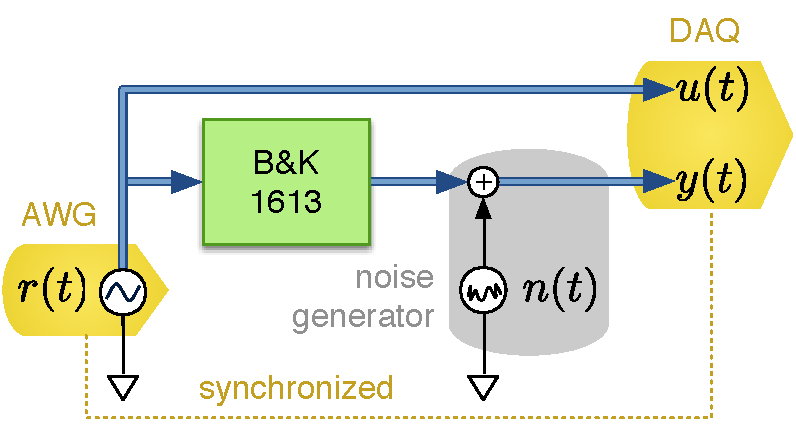
\includegraphics[width=0.8\onecolumnwidth]{\thisDir/fig/measurement.pdf}
  \caption[Measurement schematic of \BK\ 1613 filter.]{Schematic representation of the measurement set-up for the \BK\ 1613 filter. The AWG (Arbitrary Waveform Generator) and DAQ (Data Acquisition) hardware share the same clock and are thus synchronized. 
  Blue arrows indicate coax cables. 
  At the output of the bandpass filter, a noise generator is added that buffers the incoming signal using a TL071 opamp and adds white noise before passing the signal to the DAQ.} 
  \label{fig:measurementSetup}
\end{figure}


To measure the transfer function, the \BK{} 1613 Filter was excited by a signal $r(t)$ and both its input $u(t)$ and output $y(t)$ were measured as shown in \figref{fig:measurementSetup}.
The output $y(t)$, however, was disturbed by a noise generator that added white noise over the frequency range $[\mathrm{DC}, 20\unit{kHz}]$.
The excitation signal $r(t)$ was white random noise with a standard deviation $\sigma_r = 0.25 \unit{V}$, consisting of $N_S = 8\,192$ samples, and sampled at $92 \unit{kHz}$.
The same noise sequence was repeated $N_R = 100$ times in succession, such that a non-parametric estimate of the noise could be obtained and the performance of the methods could be gauged over these different repetitions.
To distinguish the different repetitions, we denote the $r^{\text{th}}$ repetition of the $u$ signal as $u^{[r]}(t)$ (and similarly for $y(t)$).
The signal generation and acquisition was by means of a National Instruments Elvis II, using the respective \code{AO} and \code{AI} pins on the breadboard, which were wired to BNC connectors.
Although acquisition and generation were synchronized, there was a small delay $\tau = 9\unit{\mu s}$ between the acquisition of the input $u(t)$ and the output $y(t)$.
The output spectrum $Y(\omega)$ was multiplied by $\exp\left(-j\omega\tau \right)$ such that the delay-compensated $y(t)$ could be obtained using the \gls{IDFT}.

\begin{figure}
  \centering
  \setlength{\figurewidth}{0.75\onecolumnwidth}
  \setlength{\figureheight}{0.68\figurewidth}
  %% This file was created by matlab2tikz.
%
%workdir  : /Users/egon/Dropbox/VUB/PhD/Mikaya/initialvalues
%git info : commit 738172a88e3110ebbaa770c63b1b0198fe9ecd02
%           Author: Egon Geerardyn <egon.geerardyn@gmail.com>
%           Date:   Tue Feb 16 20:07:07 2016 +0100
%           
%               Revert to actual timing mode
%           
%            testRuntimes.m | 4 ++--
%            1 file changed, 2 insertions(+), 2 deletions(-)
%           
%
%
% \definecolor{mycolor1}{rgb}{0.00000,1.00000,1.00000}%
% \definecolor{mycolor2}{rgb}{1.00000,1.00000,0.00000}%
% %
% \begin{tikzpicture}

% \begin{axis}[%
% width=0.951\figurewidth,
% height=\figureheight,
% at={(0\figurewidth,0\figureheight)},
% scale only axis,
% xmode=log,
% xmin=1000,
% xmax=16000,
% ymin=-70,
% ymax=10,
% axis background/.style={fill=white},
% axis x line*=bottom,
% axis y line*=left,
% legend style={legend cell align=left,align=left,draw=white!15!black}
% ]
% \addplot [color=mycolor1,only marks,mark=*,mark options={solid}]
%   table[]{fig/bode-bk1613-1.tsv};
% \addlegendentry{Y/U};

% \addplot [color=blue,only marks,mark=*,mark options={solid}]
%   table[]{fig/bode-bk1613-2.tsv};
% \addlegendentry{mean Y/U};

% \addplot [color=green,only marks,mark=*,mark options={solid}]
%   table[]{fig/bode-bk1613-3.tsv};
% \addlegendentry{$\text{G}_{\text{VXI}}\text{ (normal)}$};

% \addplot [color=mycolor2,only marks,mark=*,mark options={solid}]
%   table[]{fig/bode-bk1613-4.tsv};
% \addlegendentry{$\text{G}_{\text{VXI}}\text{ (extra delay)}$};

% \addplot [color=black,solid]
%   table[]{fig/bode-bk1613-5.tsv};
% \addlegendentry{$\text{G}_{\text{ds}}$};

% \addplot [color=red,solid]
%   table[]{fig/bode-bk1613-6.tsv};
% \addlegendentry{$\text{G}_{\text{VXI}}$};

% \end{axis}
% \end{tikzpicture}%

\begin{tikzpicture}
\begin{axis}[%
width=\figurewidth,
height=\figureheight,
unbounded coords=jump,
xlabel={Frequency \axisunit{Hz}},
ylabel={Amplitude $\left| G \right|$ \axisunit{dB}},
scale only axis,
xmode=log,
grid=both,
yminorticks=true,
extra x ticks={4000},
extra x tick labels={$4000^{\vphantom{1}}$},
extra y ticks={10},
extra y tick labels={},
xmin=400,
xmax=40000,
xminorticks=true,
ymin=-80,
ymax=10,
axis x line*=bottom,
axis y line*=left]

\addplot [FRFSingle,forget plot]
  table[]{\thisDir/fig/bode-bk1613-ETFE-single.tsv};
%\addlegendentry{Y/U};
\label{leg:bk1613:ETFE}

\addplot [FRFMean,forget plot]
  table[]{\thisDir/fig/bode-bk1613-ETFE-mean.tsv};
% %\addlegendentry{mean Y/U};
\label{leg:bk1613:meanETFE}

\addplot [GVXI,mark=*,extremelytinymarkers]
  table[]{\thisDir/fig/bode-bk1613-GVXI.tsv};
%\addlegendentry{$\text{G}_{\text{VXI}}$};
\label{leg:bk1613:vxi}

\end{axis}
\end{tikzpicture}%
 %TODO: re-enable figure and make less dense
  \caption[\BK{} 1613 filter transfer function]{Transfer function of the considered \BK{} 1613 filter.
  The empirical transfer function estimates $Y^{[r]}(\omega)/U^{[r]}(\omega)$~\legref{leg:bk1613:ETFE} and its average $\tilde{Y}(\omega)/\tilde{U}(\omega)$~\legref{leg:bk1613:meanETFE} obtained from the Elvis measurements are shown together with the estimated reference model $G_{\mathrm{VXI}}$~\legref{leg:bk1613:vxi}.} 
  \label{fig:bk1613}
\end{figure}


\subsection{Identification Procedure}
The repeated nature of the experiment makes it possible to estimate the noise level from the signals non-parametrically.
The mean signal from the input $u$ is of the form:
\begin{equation}
  \tilde{u}(t) = \frac{1}{N_R} \sum_{r=1}^{N_R} u^{[r]}(t)
\end{equation}
Thus, the reduced noise influence and the approximate noise co-variances are, respectively:
\begin{align}
  \hat\sigma_{u}^2(t) &= \frac{1}{N_R - 1} 
                    \sum_{r=1}^{N_R} 
                    \left( u^{[r]}(t) - \tilde{u}(t) \right)^2 \\
%and the noise co-variances are approximately
  \hat\sigma_{yu}(t) &= \frac{1}{N_R - 1} 
                    \sum_{r=1}^{N_R} 
                    \left( y^{[r]}(t) - \tilde{y}(t) \right)
                    \overline{\left( u^{[r]}(t) - \tilde{u}(t) \right)}
  \label{eq:variancePeriodic}            
\end{align}
 
Similar calculations apply to $y(t)$ and as such, $\hat\sigma_u(t)$, $\hat\sigma_y(t)$ and $\hat\sigma_{yu}(t)$ can be estimated.
Their frequency domain counterparts $\tilde{U}(\omega)$ and $\tilde{Y}(\omega)$ are obtained by using the DFT.
The resulting empirical transfer function estimate $Y^{[r]}(\omega)/U^{[r]}(\omega)$ and its periodic average $\tilde{Y}/\tilde{U}$ are shown in \figref{fig:bk1613}.
The noise covariances $\hat\sigma^2_{U}(\omega)$, $\hat\sigma^2_{Y}(\omega)$ and  $\hat\sigma_{YU}(\omega)$ are calculated as the sample covariance, akin to equation \eqref{eq:variancePeriodic}, and their values are shown in \figref{fig:SpectraMeasurement}.
Note that the SNR at the output $\mathrm{SNR}_{y} \approx 14 \unit{dB}$ is much smaller than at the input $\mathrm{SNR}_{u} \approx 50 \unit{dB}$.

\begin{figure}
  \centering
  \setlength{\figurewidth}{0.75\onecolumnwidth}
  \setlength{\figureheight}{0.68\figurewidth}
  %% This file was created by matlab2tikz v0.4.7 (commit 742c12da8070045a639367962f5a55fd750c0cae) running on MATLAB 8.3.
% Copyright (c) 2008--2014, Nico Schlömer <nico.schloemer@gmail.com>
% All rights reserved.
% Minimal pgfplots version: 1.3
% 
% workdir  : /Users/egon/Dropbox/VUB/PhD/Mikaya/InitialValues
% git info : commit 45c2d89a4e4044db9de2834c5c1c86bec69e4864
%            Author: Egon Geerardyn <egon.geerardyn@gmail.com>
%            Date:   Tue Oct 7 09:18:45 2014 +0200
%            
%                estimParamMeas: duplicate code removed
%            
%             estimateParametricMeas.m | 9 +--------
%             1 file changed, 1 insertion(+), 8 deletions(-)
%            
% 
% 
%
\begin{tikzpicture}
\begin{axis}[%
width=0.5\figurewidth,
height=\figureheight,
scale only axis,
xmin=400,
xmax=40000,
grid=both,
xmode=log,
xlabel={Frequency (Hz)},
ymin=-50,
ymax=40,
ylabel={$\left|U(\omega)\right|$ \axisunit{dB_{V}}},
name=Uspectrum,
axis x line*=bottom,
axis y line*=left
]
% \addplot [FRFSingle,forget plot]
%     table{\thisDir/fig/elvis-spectra-1.tsv};
% \label{leg:SpectraMeasurement:U:single}
\addplot [FRFNoise,forget plot]
  table{\thisDir/fig/elvis-spectra-3.tsv};
\label{leg:SpectraMeasurement:U:noise}
\addplot [FRFMean,forget plot]
  table{\thisDir/fig/elvis-spectra-2.tsv};
\label{leg:SpectraMeasurement:U:mean}
\end{axis}
\begin{axis}[%
anchor=left of north west,
at=(Uspectrum.right of north east),
xshift=0.5em,
width=0.5\figurewidth,
height=\figureheight,
scale only axis,
grid=both,
xmin=400,
xmax=40000,
xmode=log,
xlabel={Frequency \axisunit{Hz}},
ymin=-50,
ymax=40, 
ylabel={$\left|Y(\omega)\right|$ \axisunit{dB_{V}}},
yticklabels={},
axis x line*=bottom,
axis y line*=right
]
% \addplot [FRFSingle,forget plot]
%   table{\thisDir/fig/elvis-spectra-4.tsv};
\addplot [FRFNoise,forget plot]
  table{\thisDir/fig/elvis-spectra-6.tsv};
\addplot [FRFMean,forget plot]
  table{\thisDir/fig/elvis-spectra-5.tsv};
\end{axis}
\end{tikzpicture}%

  %TODO: simplify figure
  \caption[Measured input/output spectra of \BK{} filter.]{Input $U^{[r]}(\omega)$ and output $Y^{[r]}(\omega)$ spectra~\legref[2]{leg:SpectraMeasurement:U:single} measured using the Elvis.
  \legref[2]{leg:SpectraMeasurement:U:mean}: the mean spectra $\tilde{U}$ and $\tilde{Y}$, \legref[2]{leg:SpectraMeasurement:U:noise}: noise levels $\hat\sigma_U$ and $\hat\sigma_Y$.}
  \label{fig:SpectraMeasurement}
\end{figure}

For each measurement repetition, the signals $u^{[r]}(t)$, $y^{[r]}(t)$ and the variances $\sigma_U^2(\omega)$, $\sigma_Y^2(\omega)$ are used in the maximum likelihood cost function given by equation \eqref{eq:MLEcf}.
The model chosen for the cost function comprises a numerator of third order, a denominator of sixth order and transient contribution of a fifth degree. This results in a transfer function of the form:
\begin{equation}
  \model{\bullet}(s,\theta) = \frac{\sum_{i=0}^3 b_i s^i}{\sum_{i=0}^6 a_i s^i}
\end{equation}
which is typical of a sixth-order band-pass filter.
By processing the different repetitions, a parametric fit per initialization method corresponding to the appropriate branch in \figref{fig:flowgraph}, and per repetition can be obtained. 


The following equation is constructed from the final estimates for each experiment; it gives an insight into the combined contribution to the `best' estimate from all the different initialization strategies, \emph{viz}:

\begin{equation}\label{eq:selectBest}
  \model{best} = 
    \Arg_{\hat{G}} 
    \min 
    \left\{ 
      V(\model{exist}),
      V(\model{trunc}),
      V(\model{RFIR})
    \right\}
\end{equation}
where $V(\hat{G})$ corresponds to the cost function in equation \eqref{eq:MLEcf} in the parametric estimates of $\hat{G}$.
This is also the approach followed in~\citep{FDIDENT} to combine different initial estimates.

\subsection{Reference Model Measurements}

%\JL{
Since the true model $G_0$ is not known for real-life systems, a practically viable reference model is needed.
Additional measurements were performed using a \gls{VXI} measurement setup, which allowed for a signal-to-noise ratio of more than $60\unit{dB}$. 
Virtually noiseless, these measurements provided a very high quality model of the system, denoted as $G_\mathrm{VXI}$, and used as a reference model. 
The \gls{VXI} measurement setup is summarized as follows.
\begin{itemize}
  \item Signal Generator card: \gls{VXI} HP E1445A.
  \item Acquisition cards: \gls{VXI} HP E1430A.
  \item Sampling frequency: $f_\mathrm{s} = 156\,250 \unit{Hz}$.
  \item A total of $558$ frequency bins were used for the estimation, in the excited frequency band $[0.1,20] \unit{kHz}$, with a frequency resolution of $35.7\unit{Hz}$, giving a measurement time of $28\unit{ms}$. The excitation signal was band-limited periodic noise with an \gls{RMS} of $100\unit{mV}$.
  \item The input and output signals were buffered and anti-alias filtered.
\end{itemize}
This yielded the model $G_\mathrm{VXI}$ (shown in \figref{fig:bk1613}) with a relative error  of less than $0.3\%$ in the pass-band.  Denote $\model{VXI}$ to be the parametric estimate obtained using $G_{\mathrm{VXI}}$ as an initial estimate. Furthermore, $G_\mathrm{VXI}$ was used to play the role of $G_0$ from the previous section.

\subsection{Model Estimation}
  The measurements on the NI Elvis II indicate that the high-quality starting value $G_{\mathrm{VXI}}$ led to low cost function values as shown in \figref{fig:costMeasurements} and \tabref{tbl:costMeasurements}.
  The existing methods exhibit a high spread and a high median cost function, showing that a good estimate is obtained only in about $25\%$ of the cases.
  The truncation method provides better estimates in many cases, but still suffers from a high variability.
  On the other hand, the \gls{RFIR}-based initial values have both a low median cost function and spread, and thus provide better fits in almost all cases.
  Obviously, $\model{best}$ has the lowest cost function values of all methods.
  The similarity of the results for $\model{RFIR}$ and $\model{best}$ suggests that the \gls{RFIR} provides the best estimate in most of the cases.
  This can indeed be confirmed by inspecting the different estimates per repetition of the experiment.

\begin{remark}
  In the simulations (e.g. \figref{fig:single-sim}), a $60\unit{dB}$ difference between `good' and `bad' estimates was observed.
  Such a large gap is not observed in the measurements (\figref{fig:costMeasurements} and \tabref{tbl:costMeasurements}).
  Hence, defining a success rate based on a threshold tolerance would be very sensitive to the specific value of the threshold and hence unreliable.
  Instead, the statistical location and dispersion are inspected to assess the relative performance of each method.
  Practically, the median is used as a measure of location and the \gls{IQR} is used to inspect the spread as these are far more robust to outliers than e.g. the sample mean and variance.
  These measures also have an easy interpretation: the median ($50\%$ percentile) indicates the cost function value that $50\%$ of the repetitions attain.
  On the other hand, the \gls{IQR} ($25\%$ through $75\%$ percentile) contains  exactly half of the observations.
\end{remark}
\TODO{define IQR mathmatically}

\begin{figure}[p]
  \centering
  \setlength{\figurewidth}{0.85\onecolumnwidth}
  \setlength{\figureheight}{0.68\figurewidth}
  \setlength{\figurewidth}{0.75\onecolumnwidth}
  % This file was created by matlab2tikz v0.4.7 (commit 531759ea1f2f805c5b2ec975ee93dc15fff84184) running on MATLAB 8.3.
% Copyright (c) 2008--2014, Nico Schlömer <nico.schloemer@gmail.com>
% All rights reserved.
% Minimal pgfplots version: 1.3
% 
% workdir  : /Users/egon/Dropbox/VUB/PhD/Mikaya/InitialValues
% git info : commit f9bbeb38f35d63f56a82a16c2145c8bd72f1e461
%            Author: Egon Geerardyn <egon.geerardyn@gmail.com>
%            Date:   Thu Oct 2 13:07:09 2014 +0200
%            
%                Proc meas with noise
%            
%             processAllMeasurements.m | 37 +++++++++++++++++++++++++------------
%             1 file changed, 25 insertions(+), 12 deletions(-)
%            
% 
% 
%
% defining custom colors
\begin{tikzpicture}

\begin{axis}[%
width=\figurewidth,
height=0.5\figureheight,
scale only axis,
xmin=0.5,
xmax=5.5,
name=global,
xtick={0.5,1.5,2.5,3.5,4.5,5.5},
xticklabels={{$\model{VXI}$},
             {$\model{exist}$},
             {$\model{trunc}$},
             {$\model{RFIR}$},
             {$\model{best}$}},
% extra x ticks={5.5},
% extra x tick labels={},
x tick label as interval,
xticklabels={},
ymode=log,
ymin=4000,
ymax=1e5,
yminorticks=true,
ymajorgrids=true,
yminorgrids=true,
xmajorgrids=true,
ylabel={Cost $V(\theta)$},
axis x line*=bottom,
axis y line*=left
]

\addplot [boxplotBox,fill=G0HatFill,forget plot] table {\thisDir/data/meas-cost/CostFunctionsMLE-measurement-1.tsv};
\addplot [boxplotQuantiles,color=G0Hat,forget plot] table{\thisDir/data/meas-cost/CostFunctionsMLE-measurement-2.tsv};
\addplot [individualSamples,G0Hat,G0Hatmark,forget plot] table{\thisDir/data/meas-cost/CostFunctionsMLE-measurement-3.tsv};

\addplot [boxplotBox,fill=existingFill,forget plot] table {\thisDir/data/meas-cost/CostFunctionsMLE-measurement-4.tsv};
\addplot [boxplotQuantiles,color=existing,forget plot] table{\thisDir/data/meas-cost/CostFunctionsMLE-measurement-5.tsv};
\addplot [individualSamples,existing,existingmark,forget plot] table{\thisDir/data/meas-cost/CostFunctionsMLE-measurement-6.tsv};

\addplot [boxplotBox,fill=LPMTruncFill,forget plot] table {\thisDir/data/meas-cost/CostFunctionsMLE-measurement-7.tsv};
\addplot [boxplotQuantiles,color=LPMTrunc,forget plot] table{\thisDir/data/meas-cost/CostFunctionsMLE-measurement-8.tsv};
\addplot [individualSamples,LPMTrunc,LPMTruncmark,forget plot] table{\thisDir/data/meas-cost/CostFunctionsMLE-measurement-9.tsv};

\addplot [boxplotBox,fill=RFIRFill,forget plot] table {\thisDir/data/meas-cost/CostFunctionsMLE-measurement-10.tsv};
\addplot [boxplotQuantiles,color=RFIR,forget plot] table{\thisDir/data/meas-cost/CostFunctionsMLE-measurement-11.tsv};
\addplot [individualSamples,RFIR,RFIRmark,forget plot] table{\thisDir/data/meas-cost/CostFunctionsMLE-measurement-12.tsv};

\addplot [boxplotBox,fill=bestFill,forget plot] table {\thisDir/data/meas-cost/CostFunctionsMLE-measurement-13.tsv};
\addplot [boxplotQuantiles,color=best,forget plot] table{\thisDir/data/meas-cost/CostFunctionsMLE-measurement-14.tsv};
\addplot [individualSamples,best,bestmark,forget plot] table{\thisDir/data/meas-cost/CostFunctionsMLE-measurement-15.tsv};
\end{axis}

\begin{axis}[%
width=\figurewidth,
height=0.5\figureheight,
name=detail,
anchor=north west,
at={($(global.south west) - (0pt,1.5em)$)},
scale only axis,
xmin=0.5,
xmax=5.5,
xtick={0.5,1.5,2.5,3.5,4.5,5.5},
xticklabels={{$\model{VXI}$},
             {$\model{exist}$},
             {$\model{trunc}$},
             {$\model{RFIR}$},
             {$\model{best}$}},
extra y ticks={9000},
extra y tick labels={},
scaled y ticks=false,
x tick label as interval,
ymin=4000,
ymax=9000,
yminorticks=true,
ymajorgrids=true,
yminorgrids=true,
xmajorgrids=true,
ylabel={Cost $V(\theta)$},
axis x line*=bottom,
axis y line*=left
]

\addplot [boxplotBox,fill=G0HatFill,forget plot] table {\thisDir/data/meas-cost/CostFunctionsMLE-measurement-1.tsv};
\addplot [boxplotQuantiles,color=G0Hat,forget plot] table{\thisDir/data/meas-cost/CostFunctionsMLE-measurement-2.tsv};
\addplot [individualSamples,G0Hat,G0Hatmark,forget plot] table{\thisDir/data/meas-cost/CostFunctionsMLE-measurement-3.tsv};

\addplot [boxplotBox,fill=existingFill,forget plot] table {\thisDir/data/meas-cost/CostFunctionsMLE-measurement-4.tsv};
\addplot [boxplotQuantiles,color=existing,forget plot] table{\thisDir/data/meas-cost/CostFunctionsMLE-measurement-5.tsv};
\addplot [individualSamples,existing,existingmark,forget plot] table{\thisDir/data/meas-cost/CostFunctionsMLE-measurement-6.tsv};

\addplot [boxplotBox,fill=LPMTruncFill,forget plot] table {\thisDir/data/meas-cost/CostFunctionsMLE-measurement-7.tsv};
\addplot [boxplotQuantiles,color=LPMTrunc,forget plot] table{\thisDir/data/meas-cost/CostFunctionsMLE-measurement-8.tsv};
\addplot [individualSamples,LPMTrunc,LPMTruncmark,forget plot] table{\thisDir/data/meas-cost/CostFunctionsMLE-measurement-9.tsv};

\addplot [boxplotBox,fill=RFIRFill,forget plot] table {\thisDir/data/meas-cost/CostFunctionsMLE-measurement-10.tsv};
\addplot [boxplotQuantiles,color=RFIR,forget plot] table{\thisDir/data/meas-cost/CostFunctionsMLE-measurement-11.tsv};
\addplot [individualSamples,RFIR,RFIRmark,forget plot] table{\thisDir/data/meas-cost/CostFunctionsMLE-measurement-12.tsv};

\addplot [boxplotBox,fill=bestFill,forget plot] table {\thisDir/data/meas-cost/CostFunctionsMLE-measurement-13.tsv};
\label{leg:costMeasurements:best:iqr}
\addplot [boxplotQuantiles,color=best,forget plot] table{\thisDir/data/meas-cost/CostFunctionsMLE-measurement-14.tsv};
\label{leg:costMeasurements:best:median}
\addplot [individualSamples,best,bestmark,forget plot] table{\thisDir/data/meas-cost/CostFunctionsMLE-measurement-15.tsv};
\label{leg:costMeasurements:best:data}

\end{axis}
\end{tikzpicture}%

  \caption[Cost function values over the different measurements.]{Cost function values $V(\theta)$ obtained during the different realizations of the measurement.
  The bottom plot shows a zoom of the top plot.
  For each method, the inter-quartile range~\legref{leg:costMeasurements:best:iqr}, median~\legref{leg:costMeasurements:best:median} and individual values~\legref{leg:costMeasurements:best:data} are shown.
  This implies that a lower (local) minimum of the cost function can be attained using these smoothing techniques.}
  \label{fig:costMeasurements}
\end{figure}

\begin{table}[p]
  \centering
  \caption{Observed percentiles of the cost function $V(\model{\bullet}$).}
% \begin {tabular}{crrrrr}%
\toprule \multicolumn {1}{c}{\multirow {2}{*}{\shortstack {\textsc {Method}\\\phantom {0}}}} &\multicolumn {1}{c}{\multirow {2}{*}{\shortstack [r]{\textsc {Min.}\\{$0\%$}}}} &\multicolumn {1}{c}{\multirow {2}{*}{\shortstack [r]{\vphantom {?}\\\textsc {$25\%$}}}} &\multicolumn {1}{c}{\multirow {2}{*}{\shortstack [r]{\textsc {Median}\\{$50\%$}}}} &\multicolumn {1}{c}{\multirow {2}{*}{\shortstack [r]{\vphantom {?}\\\textsc {$75\%$ }}}} &\multicolumn {1}{c}{\multirow {2}{*}{\shortstack [r]{\textsc {Max.}\\{$100\%$}}}} \\\\\midrule %
\model {VXI}&\pgfutilensuremath {4\,355}&\pgfutilensuremath {4\,442}&\pgfutilensuremath {4\,494}&\pgfutilensuremath {4\,707}&\pgfutilensuremath {9\,634}\\[3pt]%
\model {exist}&\pgfutilensuremath {4\,345}&\pgfutilensuremath {4\,526}&\pgfutilensuremath {8\,741}&\pgfutilensuremath {12\,413}&\pgfutilensuremath {29\,237}\\[3pt]%
\model {trunc}&\pgfutilensuremath {4\,336}&\pgfutilensuremath {4\,476}&\pgfutilensuremath {4\,842}&\pgfutilensuremath {8\,130}&\pgfutilensuremath {88\,308}\\[3pt]%
\model {RFIR}&\pgfutilensuremath {4\,329}&\pgfutilensuremath {4\,422}&\pgfutilensuremath {4\,469}&\pgfutilensuremath {4\,716}&\pgfutilensuremath {9\,607}\\[3pt]%
\model {best}&\pgfutilensuremath {4\,329}&\pgfutilensuremath {4\,415}&\pgfutilensuremath {4\,458}&\pgfutilensuremath {4\,644}&\pgfutilensuremath {8\,570}\\\bottomrule %
\end {tabular}%

\pgfplotstabletypeset[precision=0]{
method            P000     P025     P050      P075       P100   
\model{VXI}       4354.83  4442.31  4493.52   4706.61    9633.53
\model{exist}     4345.3   4525.82  8740.54  12413.3    29236.5
\model{trunc}     4335.68  4476.29  4841.74   8130.28   88308.1
\model{RFIR}      4328.93  4422.11  4468.8    4716.46    9606.54
\model{best}      4328.93  4414.87  4457.91   4644.07    8569.93 
}
  \label{tbl:costMeasurements}
\end{table}



\subsection{Model Validation}
\subsubsection{Cost function limitations}
In the previous section, the cost function was studied to determine the effectiveness of the starting values.
However, inspecting the cost function $V(\theta)$ only accounts for how well an estimated model fits the measured data, which may be misleading.
For an example, overfitting a model may result in the absorption of both the systematic behavior and the noise into the model. 
Consequently, an arbitrarily small cost function may ensue although the estimated model may be virtually useless to predict the system behavior.

\subsubsection{Validation criterion}
To objectively assess the quality of an estimated model, a different criterion than the cost function is inspected.
To this end, the model is validated using the 2-norm (or distance) on the model error:
\begin{equation}
  \validationDistance{\bullet} 
  \isdef 
  \norm{\model{\bullet} - G_{\mathrm{VXI}}}
  \text{.}
  \label{eq:measurementCriterion}
\end{equation} 
This criterion indicates how well the obtained estimates $\model{\bullet}$ are able to describe the transfer function of the bandpass filter as observed in the validation measurement on the VXI.

\subsubsection{Validation performance}
The observed median and IQR of the distances in \figref{fig:validationMeasurements} and \tabref{tbl:validationMeasurements} have a similar qualitative interpretation as the cost function on the estimation data.
The existing methods provide good estimates in only $25\%$ of the cases.
The truncation method provides a considerable improvement but still suffers from $25\%$ poor estimates.
Compared to the existing BTLS and GTLS techniques, the RFIR and hence also $\model{best}$ entail an overall reduction in the observed distance by a factor $8$, in most cases. 
On the other hand, the reference $\model{VXI}$ shows the best global performance. 
This indicates that the proposed methods do no converge to the same local optimum.
Nevertheless, the proposed methods improve the model quality by almost an order of magnitude.

As the criterion in equation~\eqref{eq:measurementCriterion} no longer depends on the cost function, the initial estimates can also be investigated.
The difference between the distance of $\model[init]{\bullet}$ and $\model{\bullet}$ indicates how much the final ML estimate from the raw data, in each respective branch of \figref{fig:flowgraph}, improves over the initial estimate.
Remarkably, on average, the final ML estimation provides only a marginal improvement for the RFIR. 
However, this final step reduces the spread and hence yields a more reliable estimate.
E.g. note in \tabref{tbl:validationMeasurements} that this step reduces the worst-case distance from $18.21$ to $4.55$.


\begin{figure}[p]
  \centering
  \setlength{\figurewidth}{0.85\onecolumnwidth}
  \setlength{\figureheight}{0.68\figurewidth}
  \setlength{\figurewidth}{0.75\onecolumnwidth}
  % This file was created by matlab2tikz v0.4.7 (commit 742c12da8070045a639367962f5a55fd750c0cae) running on MATLAB 8.3.
% Copyright (c) 2008--2014, Nico Schlömer <nico.schloemer@gmail.com>
% All rights reserved.
% Minimal pgfplots version: 1.3
% 
% workdir  : /Users/egon/Dropbox/VUB/PhD/Mikaya/InitialValues
% git info : commit 45c2d89a4e4044db9de2834c5c1c86bec69e4864
%            Author: Egon Geerardyn <egon.geerardyn@gmail.com>
%            Date:   Tue Oct 7 09:18:45 2014 +0200
%            
%                estimParamMeas: duplicate code removed
%            
%             estimateParametricMeas.m | 9 +--------
%             1 file changed, 1 insertion(+), 8 deletions(-)
%            
% 
% 
%
% defining custom colors
\begin{tikzpicture}

\begin{axis}[%
name=global,
width=\figurewidth,
height=0.5\figureheight,
scale only axis,
xmin=0.5,
xmax=7.5,
x tick label as interval,
xtick={0.5,1.5,2.5,3.5,4.5,5.5,6.5,7.5},
xticklabels={{$\model{VXI}$},
             {$\model{exist}$},
             {$\model{trunc}^{\mathrm{init}}$},
             {$\model{trunc}$},
             {$\model{RFIR}^{\mathrm{init}}$},
             {$\model{RFIR}$},
             {$\model{best}$}},
xticklabels={},
ymode=log,
ymin=0.4,
ymax=100,
yminorticks=true,
grid=both,
% extra y ticks={120},
% extra y tick labels={},
ylabel={$\norm[2]{\model{\bullet} - G_{\mathrm{VXI}} }$},
axis x line*=bottom,
axis y line*=left
]
\addplot[dashed, black, forget plot] table[row sep=crcr]{%
0   81.555\\
10  81.555\\
};
\label{leg:validationMeasurements:H2Norm}

\addplot[area legend,solid,fill=G0HatFill,opacity=0.7,draw=none,forget plot]
table {\thisDir/fig/data/meas-validation/meas-validation-1.tsv};

\addplot [color=G0Hat,solid,forget plot]
  table{\thisDir/fig/data/meas-validation/meas-validation-2.tsv};
\addplot [G0Hat,G0Hatmark,tinymarkers,opacity=0.7,only marks,forget plot]
  table{\thisDir/fig/data/meas-validation/meas-validation-3.tsv};

\addplot[area legend,solid,fill=existingFill,opacity=0.7,draw=none,forget plot]
table {\thisDir/fig/data/meas-validation/meas-validation-4.tsv};

\addplot [color=existing,solid,forget plot]
  table{\thisDir/fig/data/meas-validation/meas-validation-5.tsv};
\addplot [existing,existingmark,tinymarkers,opacity=0.7,only marks,forget plot]
  table{\thisDir/fig/data/meas-validation/meas-validation-6.tsv};

\addplot[area legend,opacity=0.15,fill=LPMTruncInit,draw=none,forget plot]
table {\thisDir/fig/data/meas-validation/meas-validation-7.tsv};

\addplot [LPMTruncInit,solid,forget plot]
  table{\thisDir/fig/data/meas-validation/meas-validation-8.tsv};
\addplot [LPMTruncInitmark,color=LPMTruncInit,tinymarkers,opacity=0.7,only marks,forget plot]
  table{\thisDir/fig/data/meas-validation/meas-validation-9.tsv};

\addplot[area legend,solid,fill=LPMTruncFill,opacity=0.7,draw=none,forget plot]
table {\thisDir/fig/data/meas-validation/meas-validation-10.tsv};

\addplot [color=LPMTrunc,solid,forget plot]
  table{\thisDir/fig/data/meas-validation/meas-validation-11.tsv};
\addplot [LPMTrunc,LPMTruncmark,tinymarkers,opacity=0.7,only marks,forget plot]
  table{\thisDir/fig/data/meas-validation/meas-validation-12.tsv};

\addplot[area legend,opacity=0.15,fill=RFIRInit,draw=none,forget plot]
table {\thisDir/fig/data/meas-validation/meas-validation-13.tsv};

\addplot [RFIRInit,solid,forget plot]
  table{\thisDir/fig/data/meas-validation/meas-validation-14.tsv};
\addplot [RFIRInit,RFIRInitmark,tinymarkers,opacity=0.7,only marks,forget plot]
  table{\thisDir/fig/data/meas-validation/meas-validation-15.tsv};

\addplot[area legend,solid,fill=RFIRFill,opacity=0.7,draw=none,forget plot]
table {\thisDir/fig/data/meas-validation/meas-validation-16.tsv};

\addplot [color=RFIR,solid,forget plot]
  table{\thisDir/fig/data/meas-validation/meas-validation-17.tsv};
\addplot [RFIR,RFIRmark,tinymarkers,only marks,opacity=0.7,forget plot]
  table{\thisDir/fig/data/meas-validation/meas-validation-18.tsv};

\addplot[area legend,solid,fill=bestFill,opacity=0.7,draw=none,forget plot]
table {\thisDir/fig/data/meas-validation/meas-validation-19.tsv};
\label{leg:validationMeasurements:best:iqr}

\addplot [color=best,solid,forget plot]
  table{\thisDir/fig/data/meas-validation/meas-validation-20.tsv};
\label{leg:validationMeasurements:best:median}
\addplot [best,bestmark,tinymarkers,only marks,opacity=0.7,forget plot]
  table{\thisDir/fig/data/meas-validation/meas-validation-21.tsv};
\label{leg:validationMeasurements:best:data}
\end{axis}

\begin{axis}[%
name=detail,
anchor=north west,
at={($(global.south west) - (0pt,1.5em)$)},
width=\figurewidth,
height=0.5\figureheight,
scale only axis,
xmin=0.5,
xmax=7.5,
x tick label as interval,
xtick={0.5,1.5,2.5,3.5,4.5,5.5,6.5,7.5},
xticklabels={{$\model{VXI}$},
             {$\model{exist}$},
             {$\model[init]{trunc}$},
             {$\model{trunc}$},
             {$\model[init]{RFIR}$},
             {$\model{RFIR}$},
             {$\model{best}$}},
ymin=0.45,
ymax=3,
yminorticks=true,
grid=major,
%extra y ticks={30},
%extra y tick labels={},
ylabel={$\norm[2]{\model{\bullet} - G_{\mathrm{VXI}} }$},
axis x line*=bottom,
axis y line*=left
]

\addplot[area legend,solid,fill=G0HatFill,opacity=0.7,draw=none,forget plot]
table {\thisDir/fig/data/meas-validation/meas-validation-1.tsv};

\addplot [color=G0Hat,solid,forget plot]
  table{\thisDir/fig/data/meas-validation/meas-validation-2.tsv};
\addplot [G0Hat,G0Hatmark,tinymarkers,opacity=0.7,only marks,forget plot]
  table{\thisDir/fig/data/meas-validation/meas-validation-3.tsv};

\addplot[area legend,solid,fill=existingFill,opacity=0.7,draw=none,forget plot]
table {\thisDir/fig/data/meas-validation/meas-validation-4.tsv};

\addplot [color=existing,solid,forget plot]
  table{\thisDir/fig/data/meas-validation/meas-validation-5.tsv};
\addplot [existing,existingmark,tinymarkers,opacity=0.7,only marks,forget plot]
  table{\thisDir/fig/data/meas-validation/meas-validation-6.tsv};

\addplot[area legend,opacity=0.15,fill=LPMTruncInit,draw=none,forget plot]
table {\thisDir/fig/data/meas-validation/meas-validation-7.tsv};

\addplot [LPMTruncInit,solid,forget plot]
  table{\thisDir/fig/data/meas-validation/meas-validation-8.tsv};
\addplot [LPMTruncInitmark,color=LPMTruncInit,tinymarkers,opacity=0.7,only marks,forget plot]
  table{\thisDir/fig/data/meas-validation/meas-validation-9.tsv};

\addplot[area legend,solid,fill=LPMTruncFill,opacity=0.7,draw=none,forget plot]
table {\thisDir/fig/data/meas-validation/meas-validation-10.tsv};

\addplot [color=LPMTrunc,solid,forget plot]
  table{\thisDir/fig/data/meas-validation/meas-validation-11.tsv};
\addplot [LPMTrunc,LPMTruncmark,tinymarkers,opacity=0.7,only marks,forget plot]
  table{\thisDir/fig/data/meas-validation/meas-validation-12.tsv};

\addplot[area legend,opacity=0.15,fill=RFIRInit,draw=none,forget plot]
table {\thisDir/fig/data/meas-validation/meas-validation-13.tsv};

\addplot [RFIRInit,solid,forget plot]
  table{\thisDir/fig/data/meas-validation/meas-validation-14.tsv};
\addplot [RFIRInit,RFIRInitmark,tinymarkers,opacity=0.7,only marks,forget plot]
  table{\thisDir/fig/data/meas-validation/meas-validation-15.tsv};

\addplot[area legend,solid,fill=RFIRFill,opacity=0.7,draw=none,forget plot]
table {\thisDir/fig/data/meas-validation/meas-validation-16.tsv};

\addplot [color=RFIR,solid,forget plot]
  table{\thisDir/fig/data/meas-validation/meas-validation-17.tsv};
\addplot [RFIR,RFIRmark,tinymarkers,only marks,opacity=0.7,forget plot]
  table{\thisDir/fig/data/meas-validation/meas-validation-18.tsv};

\addplot[area legend,solid,fill=bestFill,opacity=0.7,draw=none,forget plot]
table {\thisDir/fig/data/meas-validation/meas-validation-19.tsv};

\addplot [color=best,solid,forget plot]
  table{\thisDir/fig/data/meas-validation/meas-validation-20.tsv};
\addplot [best,bestmark,tinymarkers,only marks,opacity=0.7,forget plot]
  table{\thisDir/fig/data/meas-validation/meas-validation-21.tsv};
\end{axis}
\end{tikzpicture}%

  \caption[Validation cost of the different measurements.]{Validation of the measured models. 
  For each method, the distance \eqref{eq:measurementCriterion} between the estimates and $\model{VXI}$ is shown~\legref{leg:validationMeasurements:best:data} together with the median~\legref{leg:validationMeasurements:best:median} and inter-quartile range~\legref{leg:validationMeasurements:best:iqr}.
  $\norm{G_{\mathrm{VXI}}}$\legref{leg:validationMeasurements:H2Norm} is shown as a reference.
  The bottom plot shows a zoom of the top plot.
  The proposed methods yield models that are closer to $\model{VXI}$ than the existing $\model{exist}$.
  The results are in line with the values of the cost function in \figref{fig:costMeasurements}.}
  \label{fig:validationMeasurements}
\end{figure}
\begin{table}[p]
  \centering
  \caption{Observed percentiles of the validation distance $\norm{\model{\bullet}-G_{\mathrm{VXI}}}$.}
% \begin {tabular}{crrrrr}%
\toprule \multicolumn {1}{c}{\multirow {2}{*}{\shortstack {\textsc {Method}\\\phantom {0}}}} &\multicolumn {1}{c}{\multirow {2}{*}{\shortstack [r]{\textsc {Min.}\\{$0\%$}}}} &\multicolumn {1}{c}{\multirow {2}{*}{\shortstack [r]{\vphantom {?}\\\textsc {$25\%$}}}} &\multicolumn {1}{c}{\multirow {2}{*}{\shortstack [r]{\textsc {Median}\\{$50\%$}}}} &\multicolumn {1}{c}{\multirow {2}{*}{\shortstack [r]{\vphantom {?}\\\textsc {$75\%$ }}}} &\multicolumn {1}{c}{\multirow {2}{*}{\shortstack [r]{\textsc {Max.}\\{$100\%$}}}} \\\\\midrule %
\model {VXI}&\pgfutilensuremath {0.47}&\pgfutilensuremath {0.92}&\pgfutilensuremath {1.06}&\pgfutilensuremath {1.29}&\pgfutilensuremath {2.41}\\[3pt]%
\model {exist}&\pgfutilensuremath {1.48}&\pgfutilensuremath {1.88}&\pgfutilensuremath {13.72}&\pgfutilensuremath {19.31}&\pgfutilensuremath {26.80}\\[3pt]%
\model [init]{trunc}&\pgfutilensuremath {1.35}&\pgfutilensuremath {2.72}&\pgfutilensuremath {14.94}&\pgfutilensuremath {24.72}&\pgfutilensuremath {85.34}\\[3pt]%
\model {trunc}&\pgfutilensuremath {1.27}&\pgfutilensuremath {1.72}&\pgfutilensuremath {2.35}&\pgfutilensuremath {13.03}&\pgfutilensuremath {63.84}\\[3pt]%
\model [init]{RFIR}&\pgfutilensuremath {1.11}&\pgfutilensuremath {1.61}&\pgfutilensuremath {1.78}&\pgfutilensuremath {2.00}&\pgfutilensuremath {18.21}\\[3pt]%
\model {RFIR}&\pgfutilensuremath {1.21}&\pgfutilensuremath {1.57}&\pgfutilensuremath {1.72}&\pgfutilensuremath {1.85}&\pgfutilensuremath {4.55}\\[3pt]%
\model {best}&\pgfutilensuremath {1.21}&\pgfutilensuremath {1.56}&\pgfutilensuremath {1.72}&\pgfutilensuremath {1.85}&\pgfutilensuremath {15.01}\\\bottomrule %
\end {tabular}%


\pgfplotstabletypeset[precision=2,zerofill=true]{
method              P000      P025      P050        P075     P100   
\model{VXI}         0.47325   0.916589   1.06396   1.29177   2.4089
\model{exist}       1.48252   1.88392   13.7177   19.3113   26.7984
\model[init]{trunc} 1.35399   2.72412   14.9431   24.7154   85.3351
\model{trunc}       1.27344   1.71872    2.34574  13.0301   63.8373
\model[init]{RFIR}  1.10525   1.61051    1.7778    2.00318  18.211
\model{RFIR}        1.20554   1.57398    1.72416   1.84941   4.55004
\model{best}        1.20554   1.55725    1.72059   1.84593  15.0063
}
\label{tbl:validationMeasurements}
\end{table}

\section{Remark on Generality}
\label{se:Generality}
In the previous sections, the usefulness of smoothing techniques to obtain initial values has been illustrated on example systems.
Other systems, e.g. discrete-time low-pass, high-pass, band-pass and band-stop filters of tenth order generated by the \code{cheby1}, \code{cheby2}, \code{ellip} and \code{butter} commands in \MATLAB{} have also been tried.

No cases were observed where using the smoothing to obtain initial values worsens the obtained model quality when the candidate model with the lowest cost function value is used (as in \eqref{eq:selectBest}).
On the contrary, significant improvements were often achieved by including the initial values from the smoothed FRF and by combining different strategies.

The usefulness of particular initial estimates, e.g. $\model[init]{RFIR}$ is obviously linked to the appropriateness of the non-parametric smoother in the experimental conditions at hand.
However, it is beyond the scope of this paper to determine which particular smoother is optimal in some specific circumstance.

\TODO{figures from review letter}

\section{Conclusion}\label{se:Conclusion}
The simulations have demonstrated that use of a smoothed non-parametric estimate of the \gls{FRF} can improve the success rate of minimizing the \gls{ML} cost function for the estimation of the transfer functions of \gls{LTI} systems, subjected to noisy signals. Specifically, two smoothing methods were used and compared: 1) the truncated \gls{LPM} method, and 2) the \gls{RFIR} method. The simulation results clearly show that the \gls{RFIR} method is superior to the truncated \gls{LPM} method and the existing \gls{BTLS} and \gls{GTLS} methods.

The usefulness of the initial values obtained via the proposed smoothing techniques was confirmed on a measurement of a band-pass filter in a noisy environment.
In most cases, the proposed initial values in the example made it possible to reduce the cost function by a factor two compared to existing methods.
Moreover, the obtained models were validated against a high-quality measurement where the \gls{RMS} error on the transfer function could be reduced by a factor of eight for most cases, due to the improved initial values.

Thus, the work in this paper has demonstrated the effectiveness of the studied \gls{FRF} smoothing techniques in enhancing the initial values.
Consequently, the ease-of-use of parametric model fitting is increased considerably by making it possible to obtain good parametric models without requiring any user interaction.
